\documentclass[english,fleqn,allpages]{ISTE_science}[2018/07/30]


\setcounter{MaxMatrixCols}{30}
\usepackage{amsthm}
%\usepackage{OKS_ISTE}
%\CropMarksOn
\usepackage{natbib}
\renewcommand\bibsection{\section{\bibname}}
\setlength{\bibsep}{3pt} 
\makeatletter

%\newcounter{numdef}[chapter] \global\long\def\thenumdef{\thechapter.\arabic{numdef}}
% \global\long\def\NumberedDefinition#1


\newsavebox{\fminibox} \newlength{\fminilength} \newenvironment{fminipage}[1][\linewidth]{%
 \setlength{\fminilength}{#1 - 2\fboxsep - 2\fboxrule}
 \begin{lrbox}{\fminibox}
  \begin{minipage}{\fminilength}}{%
  \end{minipage}
 \end{lrbox}
 \noindent
 \fbox{\usebox{\fminibox}}}


%\title{Hierarchy and co-evolution processes}
\title{Hiérarchies et processus de co-évolution dans les systèmes urbains}
%
%\maketitle
%Rheology of non-spherical particle suspensions]%{%
%Setting Monographs and Edited Collections\\
%According to the \hermes{} Guidelines\\
%with the \oh{} Package}


%\author{%
%Roger \Name{Rousseau} (class, styles, and tools design)\\[2pt]
%Christian \Name{Scheen} (English documentation)}


%\date{%
%Version~\PackageVersion{}, \filedate{}}

\def\thelanguage{1}

\usepackage{xparse}
\usepackage{ifthen}
\newcommand{\bpar}[2]{
    \ifthenelse{\thelanguage=0}{#1}{}
    \ifthenelse{\thelanguage=1}{#2}{}
}

%\usepackage[utf8]{inputenc}
%\usepackage[T1]{fontenc}




\begin{document}
\raggedbottom
%\hbadness=2000 \emergencystretch=2em \lefthyphenmin=3 \righthyphenmin=3

%\frontmatter

%\maketitle
%\tableofcontents

%\raggedbottom
\mainmatter
%\setcounter{chapter}{9}

\bpar{
\chapter{Hierarchy and co-evolution processes in urban systems}
}{
\chapter{Hiérarchies et processus de co-évolution dans les systèmes urbains}
}

%{Juste \Name{Raimbault}}
%\label{chap-struct}


%\bpar{
%\markboth{Hierarchy and co-evolution processes in urban systems}{Hierarchy and co-evolution processes in urban systems}
%}{
\markboth{Hiérarchies et processus de co-évolution dans les systèmes urbains}{Hiérarchies et processus de co-évolution dans les systèmes urbains}
%}


\authorname{Juste \Name{Raimbault}}{Center for Advanced Spatial Analysis, University College London}


% book subject "Centralités et hiérarchies des réseaux et des territoires"
% => specific geo of networks and territories


\vspace{2cm}

\begin{center}
\FonteSectionI
\bpar{
Abstract
}{
Résumé
}
\end{center}

%\medskip


\bpar{
The concept of hierarchy in complex systems is tightly linked to co-evolutionary processes. We propose here to explore it in the case of the co-evolution between transportation networks and territories. More precisely, we extend a co-evolution model for systems of cities and infrastructure networks, and systematically study its behavior following specific hierarchy indicators we introduce. We show that population hierarchy and network hierarchy are tightly linked, but that a broad range of regimes can exist. Model exploration furthermore yields non-trivial stylized facts which can be taken into account for territorial planning on such long time scales with co-evolutionary processes.
}{
Le concept de hiérarchie dans les systèmes complexes est étroitement lié aux processus de co-évolution. Nous proposons ici de l'explorer dans le cas de la co-évolution entre réseaux de transport et territoires. Plus précisément, nous étendons un modèle de co-évolution pour les systèmes de villes et les réseaux d'infrastructures, et étudions systématiquement son comportement en appliquant des indicateurs de hiérarchies spécifiques que nous introduisons. Nous montrons que la hiérarchie des population et celle du réseaux sont fortement liées, mais qu'une large gamme de régimes peuvent exister. L'exploration du modèle produit de plus des faits stylisés non triviaux qui peuvent être pris en compte pour la planification territoriale sur de telles échelles de temps long avec des processus de co-évolution.
}


%\bigskip

\cite{pumain1982chemin}

\cite{salthe2012hierarchical}
\cite{battyalexander}


%%%%%%%%%%%%%%%%
\bpar{
\section{Introduction}
}{
\section{Introduction}
}


\bpar{
\subsection{Complexity and hierarchy}
}{
\subsection{Complexité et hiérarchie}
}


\bpar{
Complex systems with emergent properties produced by self-organization processes are also most of the time exhibiting some kind of hierarchical structure. Although the term of hierarchy has several different definitions and uses in very different disciplines, ranging from political science \citep{crumley1987dialectical} to physics \citep{10.1371/journal.pone.0033799}, it seems to be intrinsically linked with complexity. \cite{lane2006hierarchy} classifies four frequent uses of the term hierarchy, namely (i) order hierarchy corresponding to the existence of an order relation for a set of elements, (ii) inclusion hierarchy which is a recursive inclusion of elements within each other, (iii) control hierarchy which is the ``common sense'' use of the term as ranked entities controlling other entities with lower rank, and (iv) level hierarchy which captures the multi-scale nature of complex systems as ontologically distinct levels (or scales). For the particular study of social systems, he concludes that hierarchical levels may be entangled, that upward and downward causations are both essential, and that at least three levels (micro, meso, macro) are generally needed to capture the complexity of such systems. In a more philosophical account of complexity, \cite{morin1980methode} constructs a hierarchical method of interdisciplinary knowledge, insists on the tension between dependancy and interdependency or between opening and closing (rejoining ideas from \cite{holland2012signals}), and develops an implicit hierarchy of social systems when hypothesizing the emergence of third-type societies (swarm intelligence between humans).
}{
Les systèmes complexes avec propriétés émergentes produites par des processus d'auto-organisation présentent aussi dans la plupart des cas une certaine structure hiérarchique. Même si le terme de hiérarchie a différentes définitions et usages dans des disciplines très différentes, qui s'étendent des sciences politiques \citep{crumley1987dialectical} à la physique \citep{10.1371/journal.pone.0033799}, il semble être intrinsèquement lié à la complexité. \cite{lane2006hierarchy} classifie quatre usages fréquents du terme de hiérarchie, qui sont (i) la hiérarchie d'ordre qui correspond à l'existence d'une relation d'ordre pour un ensemble d'éléments, (ii) la hiérarchie d'inclusion qui est une inclusion récursive d'éléments les uns dans les autres, (iii) la hiérarchie de contrôle qui est l'usage du terme au ``sens commun'' comme des entités avec un rang contrôlant les autres entités avec un plus petit rang, et (iv) la hiérarchie de niveau qui capture la nature multi-scalaire des systèmes complexes comme des niveaux ontologiquement distincts (ou échelles). Pour l'étude des systèmes sociaux en particulier, il conclut que les niveaux hiérarchiques peuvent être intriqués, que les causalités vers le haut et vers le bas sont toutes les deux essentielles, et que au moins trois niveaux (micro, meso, macro) sont généralement nécessaires pour capturer la complexité de tels systèmes. D'un point de vue plus philosophique sur la complexité, \cite{morin1980methode} construit une méthode hiérarchique de la connaissance interdisciplinaire, insiste sur la tension entre dépendance et interdépendance, ou entre ouverture et fermeture (rejoignant des idées de \cite{holland2012signals}), et développe une hiérarchie implicite des systèmes sociaux en faisant l'hypothèse de l'émergence de sociétés du troisième type (intelligence collective entre humains).
}


\bpar{
Different types of complexity may be related to different types of hierarchy as \cite{raimbault:halshs-02089520} proposes, and hierarchy would indeed be endogenous to theories of complexity. \cite{allen2017multiscale} develop a multiscale information theory in which the information profile across scales, or hierarchical levels, allows quantifying the complexity of a system. The complex adaptive system theory of \cite{holland2012signals} considers complex systems as systems of boundaries that filter signals, implying an inclusion and scale hierarchy between boundaries. Theories of scaling as the one synthesized by \cite{west2017scale} rely on the quantification of hierarchy in certain dimensions of systems, captured by exponents of scaling laws. Hierarchy may be endogenous to complexity, or to knowledge of the complex itself, since for example \cite{fanelli2013bibliometric} provides empirical evidence of a ``hierarchy of sciences'', in the sense of possibility to reach theoretical and methodological consensus. This corresponds in some sense to the ``ontological complexity'' of \cite{pumain2003approche}, which relies on the number of viewpoints needed to grasp a system, or the number of perspectives in an applied perspectivism framework \citep{raimbault2020relating}. Wether linked to systems themselves or to models and theories of them, hierarchy appears to be tightly linked to complexity.
}{
Différents types de complexités peuvent être mises en relation avec différents types de hiérarchies comme \cite{raimbault:halshs-02089520} propose, et la hiérarchie serait en fait endogène aux théories de la complexité. \cite{allen2017multiscale} développent une théorie multiscalaire de l'information dans laquelle le profil de l'information entre les échelles, ou niveaux hiérarchiques, permet de quantifier la complexité d'un système. La théorie des systèmes complexes adaptatifs de \cite{holland2012signals} considère les systèmes complexes comme des ensembles de frontières qui filtrent des signaux, impliquant des hiérarchies d'inclusion et d'échelle entre les frontières. Les théories des lois d'échelle comme celle synthétisée par \cite{west2017scale} se basent sur la quantification de la hiérarchie pour certaines dimensions des systèmes, capturée par les exposants des lois d'échelle. La hiérarchie peut être endogène à la complexité, ou à la connaissance du complexe elle-même, puisque par exemple \cite{fanelli2013bibliometric} fournit des éléments empiriques témoignants d'une ``hiérarchie des sciences'', au sens d'une possibilité d'atteindre des consensus théoriques et méthodologiques. Cela correspond dans une certaine mesure à la ``complexité ontologique'' de \cite{pumain2003approche}, qui se base sur le nombre de points de vue nécessaire pour capturer un système, ou bien le nombre de perspectives dans le cadre d'un perspectivisme appliqué \citep{raimbault2020relating}. Que se soit en lien avec les systèmes eux-mêmes ou avec les modèles et théories de ceux-ci, la hiérarchie apparait être étroitement liée à la complexité.
}


\bpar{
\subsection{Territorial systems and hierarchy}
}{
\subsection{Systèmes territoriaux et hiérarchie}
}


\bpar{
Urban systems, and more generally territorial systems, are particularly linked to hierarchy \citep{pumain2006hierarchy}: they indeed encompass all the meanings aforementioned (order hierarchy between settlement sizes for example, inclusion hierarchy between territorial boundaries, control hierarchy through governance structure, and more importantly level hierarchy through their multi-scalar nature). \cite{batty2006hierarchy} shows that hierarchies are inherent to urban systems, as fat tail distribution of settlement size are already produced by simple models of urban growth, and suggests also that urban design processes imply underlying overlapping hierarchies. \cite{pumain2006alternative} links hierarchical selection and hierarchical diffusion of innovation across cities to the long-term dynamics of urban systems. \cite{pumain:halshs-02303136} recalls that interactions in systems of cities are tightly linked to the emergence of urban hierarchies. Generally, scaling laws in urban systems can be considered as systematic manifestations of a hierarchical structure \citep{pumain2004scaling}, which is more complex than a simple order hierarchy, since scaling patterns vary with the definition of cities \citep{cottineau2017diverse}.
}{
Les systèmes urbains, et plus généralement les systèmes territoriaux, sont particulièrement liés à la hiérarchie \citep{pumain2006hierarchy}: ils sont en effet concernés par l'ensemble des significations données ci-dessus (hiérarchie d'ordre entre les tailles des établissements par exemple, hiérarchie d'inclusion entre les frontières territoriales, hiérarchie de contrôle au travers des structures de gouvernance, et de manière plus importante hiérarchie de niveau par leur nature multi-scalaire). \cite{batty2006hierarchy} montre que les hiérarchies sont inhérentes aux systèmes urbains, comme des distributions à longue queue de taille d'établissements sont déjà produites par des modèles simples de croissance urbaine, et suggère aussi que les processus de design urbain impliquent des hiérarchies entrelacées sous-jacentes. \cite{pumain2006alternative} relie sélection hiérarchique et diffusion hiérarchique de l'innovation entre les villes aux dynamiques de temps long des systèmes urbains. \cite{pumain:halshs-02303136} rappelle que les interactions dans les systèmes de villes sont étroitement liées à l'émergence des hiérarchies urbaines. De manière générale, les lois d'échelle dans les systèmes urbains peuvent être considérés comme des manifestations systématiques d'une structure hiérarchique \citep{pumain2004scaling}, qui est plus complexe qu'une simple hiérarchie d'ordre, puisque les motifs de lois d'échelle varient avec la définition des villes \citep{cottineau2017diverse}.
}


\bpar{
Hierarchical properties can be observed on several dimensions of urban systems. For example, transportation systems are hierarchical in their structure \citep{yerra2005emergence} but also patterns of use such as transportation flows \citep{jiang2009street}. Urban hierarchies are tightly related to hierarchies of their transportation links \citep{bigotte2010integrated}, and different modes of transportation networks are concerned including the air network \citep{dang2012hierarchy}. The global distribution of multinational firms also exhibits strong hierarchical patterns \citep{godfrey1999ranking}. Governance structures are organized following both an inclusion hierarchy for administrative areas \citep{li2015administrative} but also level hierarchies for example for economic processes \citep{liao2017opening}. Territorial systems are therefore intrinsically hierarchical in their multiple dimensions, what is tightly linked to their different complexities \citep{2019arXiv190109869R}. 
}{
Des propriétés hiérarchiques peuvent être observées pour différentes dimensions des systèmes urbains. Par exemple, les systèmes de transport sont hiérarchiques dans leur structure \citep{yerra2005emergence} mais aussi dans leur motifs d'usage comme les flux de transport \citep{jiang2009street}. Les hiérarchies urbaines sont étroitement reliées aux hiérarchies de leur liens de transport \citep{bigotte2010integrated}, et différents modes de transport sont concernés incluant les réseaux aériens \citep{dang2012hierarchy}. La distribution globale des firmes multinationales présente également de forts motifs hiérarchiques \citep{godfrey1999ranking}. Les structures de gouvernance sont organisées suivant à la fois une hiérarchie d'inclusion pour les aires administratives  \citep{li2015administrative} mais aussi des hiérarchies de niveau par exemple pour les processus économiques \citep{liao2017opening}. Les systèmes territoriaux sont pour cela intrinsèquement hiérarchiques dans leur multiples dimensions, ce qui est étroitement lié à leurs différentes complexités \citep{2019arXiv190109869R}.
}




\bpar{
\subsection{Co-evolution and hierarchy}
}{
\subsection{Co-évolution et hiérarchie}
}



\bpar{
Hierarchy in complex systems is furthermore intrinsically linked to the concept of co-evolution. Following \cite{lane2006hierarchy}, the approach to complex adaptive systems proposed by \cite{holland2012signals} integrates levels and nested hierarchies, since it considers complex systems as ensembles of boundaries that filter signals. \cite{holland2012signals} formalizes complex adaptive systems as these structures of boundaries which form co-evolution niches for the elements and subsystems within a given boundary. The concept is slightly different from the concept of ecological niche which more generally designates a region in a parameter space quantifying the environment in which a species can live. In ecology, \cite{pires2011food} show that the emergence of mutualistic species networks imply some feeding hierarchy.
}{
La hiérarchie dans les systèmes complexes est de plus intrinsèquement liée au concept de co-évolution. Suivant \cite{lane2006hierarchy}, l'approche des systèmes complexes adaptatifs proposée par \cite{holland2012signals} intègre des niveaux et hiérarchies imbriquées, puisque elle considère les systèmes complexes comme ensembles de frontières qui filtrent les signaux. \cite{holland2012signals} formalise les systèmes complexes adaptatifs comme ces structures de frontières qui forment des niches de co-évolution pour les éléments et sous-systèmes dans une frontière donnée. Ce concept est un peu différent de celui de niche écologique qui correspond plus généralement à une région dans un espace de paramètres quantifiant l'environnement dans lequel une espèce peut vivre. En écologie, \cite{pires2011food} montre que l'émergence de réseaux d'espèces mutualistes implique une hiérarchie trophique.
}


\bpar{
In the context of economic and geographical processes, \cite{volberda2003co} distinguish for the co-evolution of firms between a genealogical hierarchy (evolutionary processes in the biological sense) and an ecological hierarchy (co-evolutionary economic processes). \cite{liu2013exploring} suggest that air networks co-evolve with firm networks and that their hierarchies are related therethrough. \cite{raimbault2019modeling} introduces a co-evolution approach to study interactions between transportation networks and territories, which from an urban system viewpoint in the sense of \cite{pumain2006evolutionary} relates to urban hierarchies. \cite{levinson2007co} confirm a correspondance between urban and network hierarchies in a co-evolution model. Within the SimpopNet model for the co-evolution of cities and networks \citep{schmitt2014modelisation}, discrete hierarchical level of network links corresponding to successively improved transportation technologies are a core component of simulation rules. \cite{raimbault2020unveiling} furthermore showed that the level of initial urban hierarchy in terms of rank-size slope had significant impacts on model outcomes. Studying hierarchies in the context of co-evolution transportation networks and territories is thus a relevant entry to the underlying concepts, including complexity, hierarchy, co-evolution and territorial systems.
}{
Dans le contexte des processus économiques et géographiques, \cite{volberda2003co} distingue pour la co-évolution des entreprises entre une hiérarchie généalogique (processus d'évolution au sens biologique) et une hiérarchie écologique (processus de co-évolution économiques). \cite{liu2013exploring} suggère que les réseaux aériens co-évoluent avec les réseaux d'entreprises et que leur hiérarchies sont en relation par ce processus. \cite{raimbault2019modeling} introduit une approache par la co-évolution pour l'étude des interactions entre réseaux de transport et territories, qui d'un point de vue des systèmes urbains au sens de \cite{pumain2006evolutionary} est en relation avec les hiérarchies urbaines. \cite{levinson2007co} confirment une correspondance entre hiérarchie urbaine et de réseau dans un modèle de co-évolution. Au sein du modèle SimpopNet pour la co-évolution des villes et des réseaux \citep{schmitt2014modelisation}, des niveaux hiérarchiques discrets de liens de réseau, correspondant à des technologies de transport améliorées successivement, sont une composante fondamentale des règles de simulation. \cite{raimbault2020unveiling} a d'autant plus montré que le niveau initial de hiérarchie urbaine en termes de loi rang-taille a un impact significatif sur les sorties du modèle. L'étude des hiérarchies dans le contexte de la co-évolution des réseaux de transport et des territoires est pour cela une entrée pertinente pour les concepts sous-jacents, incluant la complexité, la hiérarchie, la co-évolution et les systèmes territoriaux.
}


\bpar{
\subsection{Proposed approach}
}{
\subsection{Approche proposée}
}


\bpar{
\cite{pumain2006introduction} recalls in the context of social systems some remaining open methodological questions: how are hierarchies produced? How do hierarchies evolve? What discriminates between continuous and discrete hierarchical organisations? Our contribution brings new elements of answer to the first two questions above, in the particular case of co-evolution of transportation networks and territories. It situates at the intersection of the three previously given contexts, namely hierarchy in complex systems and more particularly territorial systems, seen through the prism of co-evolutive processes.
}{
\cite{pumain2006introduction} rappelle dans le contexte des systèmes sociaux certaines questions méthodologiques qui restent ouvertes: comment sont produites les hiérarchies? Comment les hiérarchies évoluent-elles? Quels facteurs sont discriminants entre des organisation hiérarchiques continues ou discrètes ? Notre contribution apporte de nouveaux éléments de réponse aux deux première questions ci-dessus, dans le cas particulier de la co-évolution des réseaux de transport et des territories. Elle se situe à l'intersection des trois contextes données précédemment, c'est-à-dire la hiérarchie dans les systèmes complexes et plus particulièrement les systèmes territoriaux, vus au travers du prisme des processus de co-évolution. 
}


\bpar{
More precisely, we propose to systematically explore a macroscopic co-evolution model for cities and networks, and study its properties regarding both hierarchies of each component, in terms of final hierarchy produced but also in terms of the relations between these hierarchies. Establishing links between microscopic processes and emergent hierarchical patterns through model exploration informs on possible drivers of these macroscopic patterns. Our contribution relies on three aspects: (i) we introduce a comprehensive set of indicators tailored to the study of hierarchy in territorial systems; (ii) we systematically explore the version with a physical network of the co-evolution model introduced by \cite{raimbault2018modeling} which only studied extensively the virtual network; and (iii) we apply a novelty search algorithm to establish the feasible space of hierarchy patterns which can be produced by the model.
}{
Plus précisément, nous proposons d'explorer systématiquement un modèle macroscopique de co-évolution entre villes et réseaux, et d'étudier ses propriétés au regard des hiérarchies de chacun des composants, en termes de hiérarchies finalement produites mais aussi en termes de relations entre ces hiérarchies. L'établissement de liens entre processus microscopiques et motifs de hiérarchie émergents par l'exploration du modèle informe sur les possibles déterminants de ces motifs macroscopiques. Notre contribution repose sur trois aspects: (i) nous introduisons un jeu d'indicateurs exhaustif spécifiques à l'étude de la hiérarchie des systèmes territoriaux; (ii) nous explorons systématiquement la version avec réseau physique du modèle de co-évolution introduit par \cite{raimbault2018modeling} qui étudiait de manière extensive seulement le réseau virtuel; et (iii) nous appliquons un algorithme de recherche de nouveauté pour établir l'espace faisable des motifs de hiérarchie qui peuvent être produits par le modèle.
}


\bpar{
The rest of this chapter is organized as follows. We first describe the model used and introduce a novel set of indicators to quantify hierarchy in territorial systems. We then describe the results of a grid exploration of the co-evolution model using these indicators, both with the physical and virtual networks, and establish the feasible space of model outputs. We finally discuss the implications of these results for hierarchy within co-evolutionary processes.
}{
La suite de ce chapitre est organisée de la façon suivante. Nous décrivons d'abord le modèle utilisé et introduisons un nouveau jeu d'indicateurs pour quantifier la hiérarchie dans les systèmes territoriaux. Nous décrivons ensuite les résultats d'une exploration par grille du modèle de co-évolution en utilisant ces indicateurs, à la fois pour le réseau physique et pour le réseau virtuel, et établissons l'espace faisable des sorties du modèle. Nous discutons finalement les implications de ces résultats pour la hiérarchie au sein des processus de co-évolution.
}


%%%%%%%%%%%%%%%%
\bpar{
\section{Co-evolution model}
}{
\section{Modèle de co-évolution}
}

\bpar{
\subsection{Context}
}{
\subsection{Contexte}
}


\bpar{
The issue of interactions between transportation networks and territories remains an open question for which different approaches have been proposed \cite{offner1993effets,espacegeo2014effets}. \cite{raimbault2018caracterisation} has explored a co-evolution approach, in the sense that both dynamics have circular causal relationships. More precisely, \cite{raimbault2019modeling} introduces a definition of co-evolution in that particular context, based on the aforementioned co-evolution niches \citep{holland2012signals}, for which an empirical characterization method based on lagged correlations is developed \citep{raimbault2017identification}. As its application on empirical data yield various or inconclusive results, the use of simulation models is a medium to indirectly link microscopic processes with a potentially emergent co-evolution, both at the mesoscopic scale \citep{raimbault2019urban} and at the macroscopic scale \citep{raimbault2018modeling}. This latest model is the one used in this study.
}{
Le problème des interactions entre réseaux de transport et territoires reste une question ouverte pour laquelle différentes approches ont été proposée \cite{offner1993effets,espacegeo2014effets}. \cite{raimbault2018caracterisation} a exploré une approche par co-évolution, au sens que les deux dynamiques ont des relations circulaires causales. Plus précisément, \cite{raimbault2019modeling} introduit une définition de la co-évolution dans ce contexte particulier, basée sur les niches de co-évolution mentionnées précédemment \citep{holland2012signals}, pour laquelle une méthode de caractérisation empirique basée sur des corrélations retardées est développée \citep{raimbault2017identification}. Comme son application sur données empiriques donne des résultats variés ou inconclusifs, l'utilisation de modèles de simulation est un medium pour lier indirectement les processus microscopiques avec une co-évolution émergente potentielle, à la fois à l'échelle mesoscopique \citep{raimbault2019urban} et à l'échelle macroscopique \citep{raimbault2018modeling}. Ce dernier modèle est celui utilisé dans cette étude.
}

\bpar{
\subsection{Model description}
}{
\subsection{Description du modèle}
}

\bpar{
The co-evolution model for cities and transportation networks at the macroscopic scale extends the spatial interaction model introduced by \cite{raimbault2018indirect} by adding dynamical speeds to network links. A system of cities is represented as cities as agents and network links between these. Interaction flows are determined with a spatial interaction model, and they determine city growth rates, while network links evolve according to the flow traversing them. See \cite{raimbault2018modeling} for a full mathematical description of the model. We describe below the specification and parameters used here.
}{
Le modèle de co-évolution pour les villes et les réseaux de transport à l'échelle macroscopique étend le modèle d'interactions spatial introduit par \cite{raimbault2018indirect} en ajoutant des vitesses dynamiques aux liens du réseau. Un système de villes est représenté par les villes comme agents et des liens du réseau entre celles-ci. Les flux d'interaction sont déterminés par un modèle d'interaction spatial, et ceux-ci déterminent les taux de croissance des villes, tandis que les liens du réseau évoluent selon le flux qui les traversent. Voir \cite{raimbault2018modeling} pour une description mathématique complète du modèle. Nous décrivons ci-dessous la spécification et les paramètres utilisés ici.
}

\bpar{
More precisely, a time step of the simulation model consists in the following steps:
\begin{enumerate}
	\item cities evolve their populations following gravity interaction flows of unit weight $w_G$, as a scaling function of population with exponent $\gamma_G$, and with a distance decay parameter $d_G$; cities do not have endogenous growth in our setting (Gibrat model) as we focus our study on interactions;
	\item flows are assigned to network links, either (i) to the direct link between the two cities in the case of the virtual network, or (ii) through a shortest path assignment algorithm (betweenness centrality) in the case of a physical network;
	\item links evolve their speed with a thresholded self-reinforcement function of flows, with maximal time travel decrease $g_M$; a threshold for flows above which (resp. below which) speed increase (resp. decrease) determined by a flow quantile parameter $\phi^{(q)}_0$; and as a scaling relation to relative flows with exponent $\gamma_N$.
\end{enumerate}
}{
Plus précisément, un pas de temps du modèle de simulation consiste en les étapes suivantes:
\begin{enumerate}
	\item les populations des villes évoluent suivant les flux d'interaction gravitaires de poids unitaire $w_G$, comme une loi d'échelle des populations avec un exposant $\gamma_G$, et avec un paramètre de décroissance de la distance $d_G$; les villes n'ont pas de croissance endogène dans notre configuration (modèle de Gibrat) puisque notre étude se concentre sur les interactions;
	\item les flux sont assignés aux liens du réseau, soit (i) au lien direct entre les deux villes dans le cas du réseau virtuel, ou (ii) par un algorithme de distribution par plus court chemin (centralité d'intermédiarité) dans le cas d'un réseau physique;
	\item les liens évoluent leur vitesse avec une fonction d'auto-renforcement par seuil en fonction des flux, avec taux maximal de croissance du temps de trajet $g_M$; un seuil pour les flux au dessus duquel (resp. en dessous duquel) la vitesse augmente (resp. diminue) déterminé par un paramètre de quantile des flux $\phi^{(q)}_0$; et comme une relation d'échelle des flux relatifs avec exposant $\gamma_N$.
\end{enumerate}
}


\bpar{
The model can be initialized with real data or by generating a synthetic initial configuration which has its own parameters \citep{raimbault2019space}. In our case, $N = 30$ cities are randomly distributed in an uniform space of width $W=200km$, and population follow a rank-size law with parameter $\alpha_S$. For the virtual network case, all pair links are initialized with pace one, while for the physical network case a perturbed grid network is used as described in \cite{raimbault2018modeling}. We show in Fig.~\ref{fig:examples} model runs for synthetic virtual and physical networks, and for the French system of cities with railway data. We visually observe that the number of important links is smaller in the physical case as it could be expected as infrastructure is shared by neighboring flows. For the real system, the most important links emerging correspond roughly to the actual existing high-speed lines.
}{
Le modèle peut être initialisé sur données réelles ou par génération d'une configuration initiale synthétique qui a ses propres paramètres \citep{raimbault2019space}. Dans notre cas, $N=30$ villes sont distribuées aléatoirement dans un espace uniforme de largeur $W=200km$, et les populations suivent une loi rang-taille avec paramètre $\alpha_S$. Dans le cas du réseau virtuel, toutes les paires de liens sont initialisés avec une allure unitaire, tandis que dans le cas du réseau physique un réseau en grille perturbé est utilisé comme décrit dans \cite{raimbault2018modeling}. Nous montrons en Fig.~\ref{fig:examples} des executions du modèle pour les réseaux virtuels et physiques, et pour le système de villes français avec les données de réseau ferré. Nous observons visuellement que le nombre de liens importants est plus petit dans le cas du réseau physique comme cela pouvait être attendu puisque l'infrastructure est partagée par des flux voisins. Pour le système réel, les liens les plus importants qui émergent correspondent globalement aux lignes à grande vitesse en effet existantes.
}


%%%%%%%%%%%%
\begin{figure}
	%\begin{center}
	%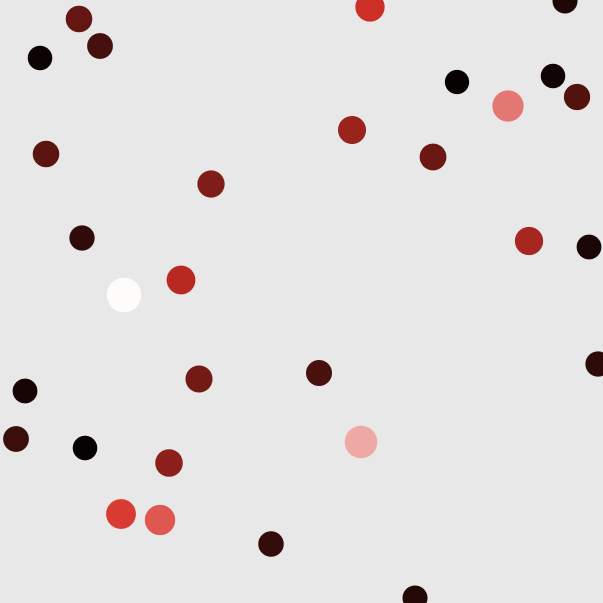
\includegraphics[width=0.48\linewidth]{figuresraw/ex_synthvirtual_1_t0.png}
	%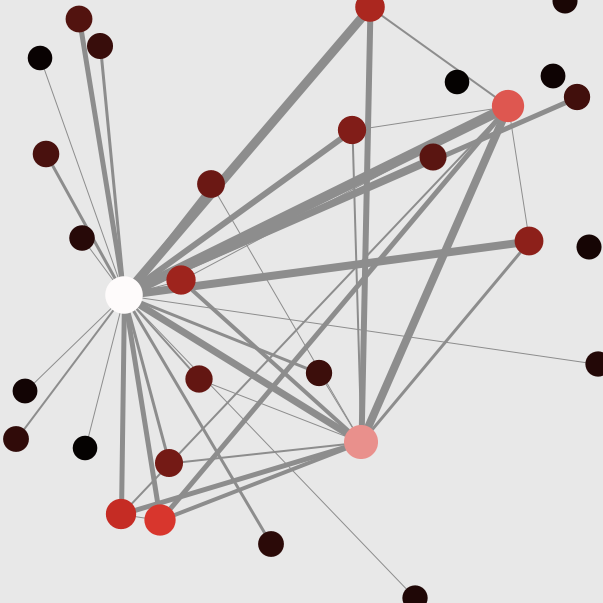
\includegraphics[width=0.48\linewidth]{figuresraw/ex_synthvirtual_1_t30.png}\\
	%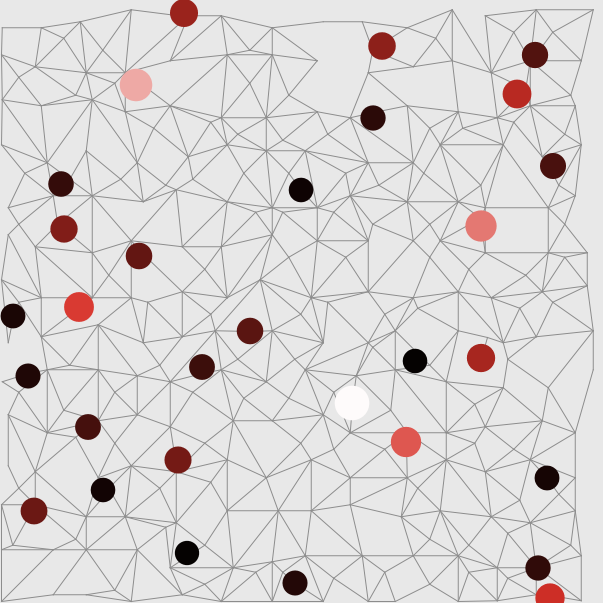
\includegraphics[width=0.48\linewidth]{figuresraw/ex_synthphysical_1_t0.png}
	%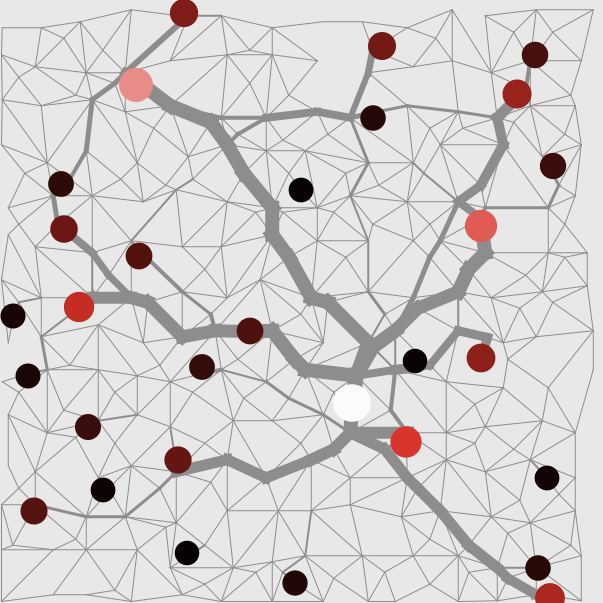
\includegraphics[width=0.48\linewidth]{figuresraw/ex_synthphysical_1_t30.png}\\
	%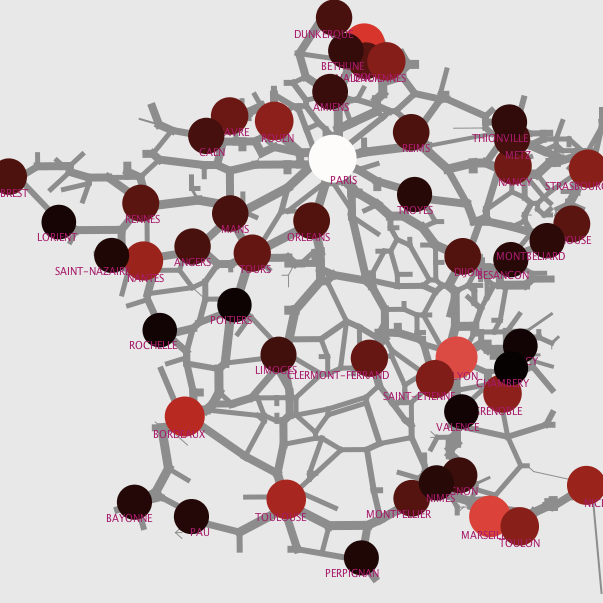
\includegraphics[width=0.48\linewidth]{figuresraw/ex_realphysical_1975_t0.png}
	%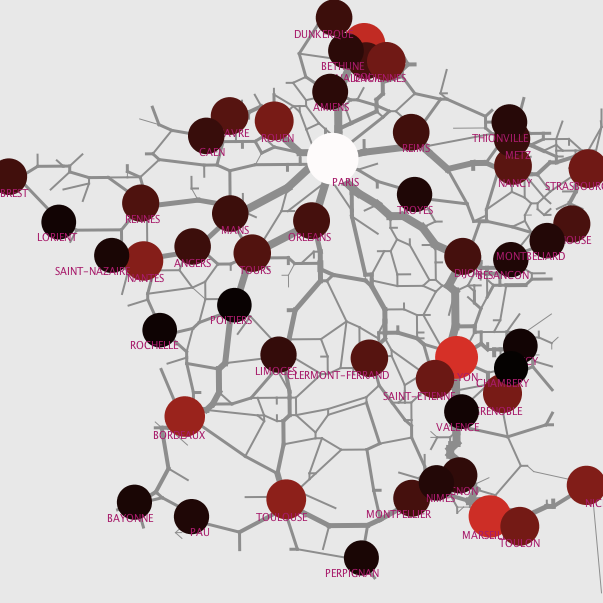
\includegraphics[width=0.48\linewidth]{figuresraw/ex_realphysical_1975_tf.png}
	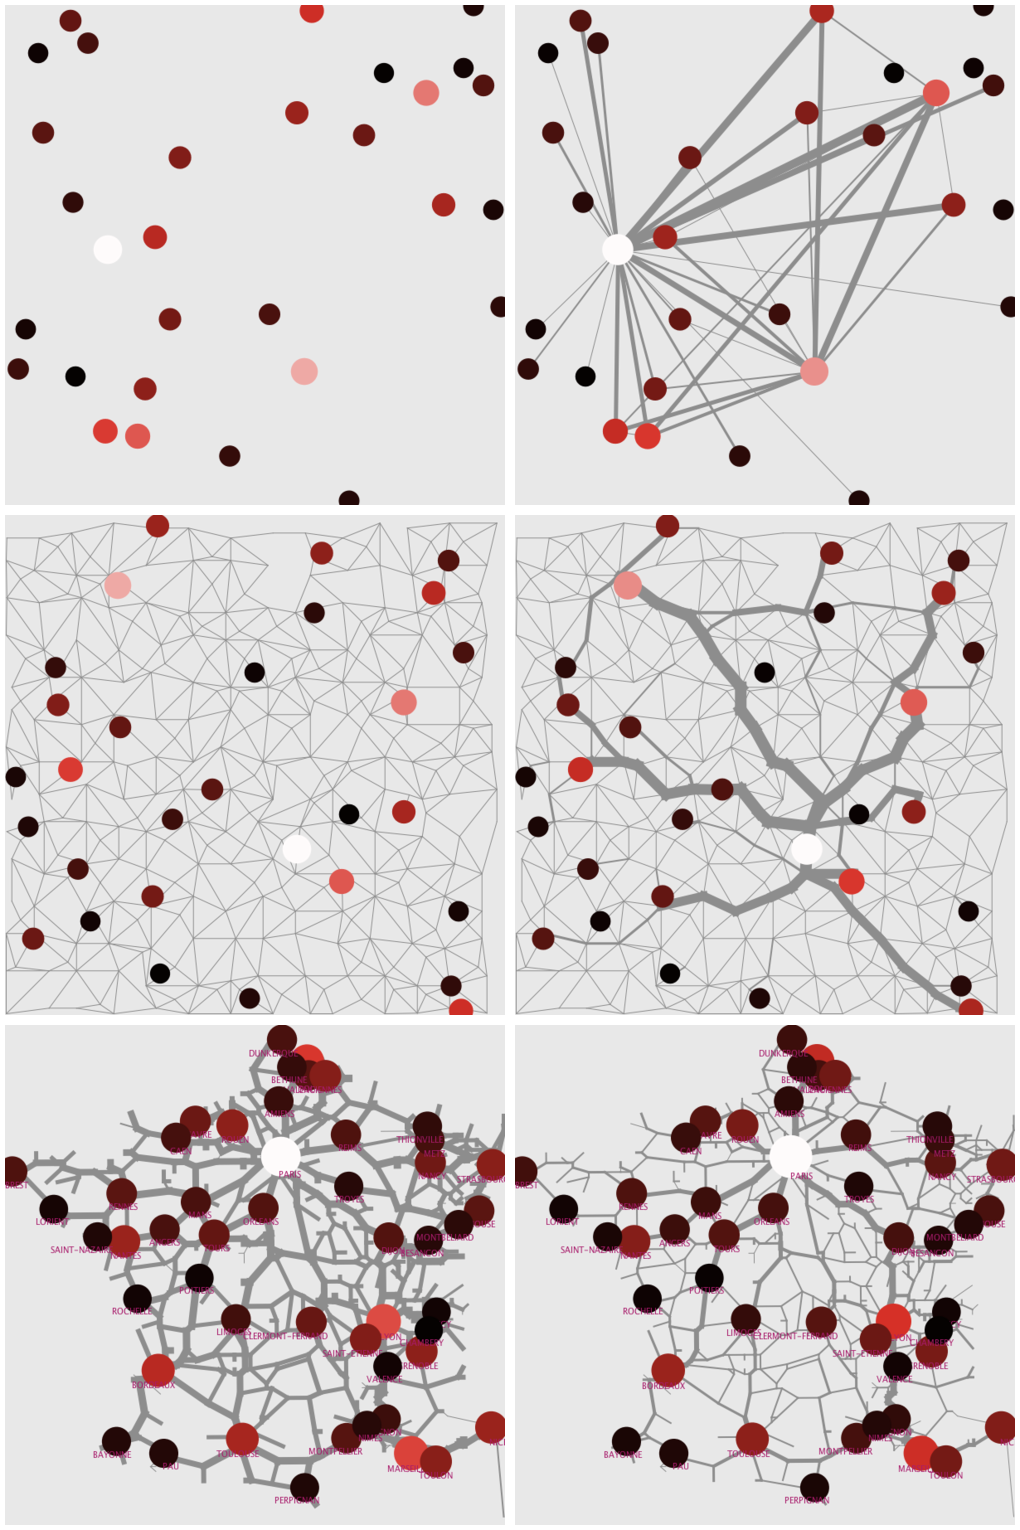
\includegraphics[width=0.95\linewidth]{figures/Fig1.png}
	%\end{center}
	\bpar{
	\caption{\footnotesize\textbf{Examples of different setups for the co-evolution model.} \textit{(Top row)} Synthetic system of cities with virtual network, initial configuration (left) and after $t_f=30$ time steps (right), with parameters $\alpha_S = 1$, $\phi^{(q)}_0 = 0.9$, $g_M = 0.01$, $\gamma_N=2$, $w_G=4.7e-3$, $d_G=248$, $\gamma_G=0.9$; \textit{(Middle row)} Synthetic system of cities with physical network, initial configuration (left) and after $t_f=30$ time steps (right), with parameters $\phi^{(q)}_0 = 0.7$, $g_M = 0.05$ and the same other parameters than the first configuration; \textit{(Bottom row)} French system of cities simulated between 1975 (left) and 1999 (right) with three time steps, with parameters $\phi^{(q)}_0 = 0.8$, $g_M = 0.2$, $\gamma_N=4$ and same others. City color and size give the population and link thickness the speed (rescaled at each time step).\label{fig:examples}}
	}{
	\caption{\footnotesize\textbf{Exemples de différentes applications du modèle de co-évolution.} \textit{(Première ligne)} Système de villes synthétique avec réseau virtuel, configuration initiale (gauche) et après $t_f = 30$ pas de temps (droite), avec paramètres $\alpha_S = 1$, $\phi^{(q)}_0 = 0.9$, $g_M = 0.01$, $\gamma_N=2$, $w_G=4.7e-3$, $d_G=248$, $\gamma_G=0.9$; \textit{Ligne du milieu} Système de villes synthétique avec réseau physique, configuration initiale (gauche) et après $t_f=30$ pas de temps (droite), avec paramètres $\phi^{(q)}_0 = 0.7$, $g_M = 0.05$ et les mêmes paramètres que pour la première configuration; \textit{(Dernière ligne)} Système de villes français simulé entre 1975 (gauche) et 1999 (droite) avec trois pas de temps, et paramètres $\phi^{(q)}_0 = 0.8$, $g_M = 0.2$, $\gamma_N=4$ et les autres similaires. La couleur et taille donne la population des villes et l'épaisseur des liens leur vitesse (renormalisée à chaque pas de temps).\label{fig:examples}}
	}
\end{figure}
%%%%%%%%%%%%


\bpar{
In our exploration settings, the model has thus seven parameters (for which we give practical boundaries in experiments): the initial population hierarchy $\alpha_S \in \left[0.1; 2.0\right]$, the gravity interaction weight $w_G \in \left[1e-4; 1e-2 \right]$, the gravity interaction hierarchy $\gamma_G \in \left[0.0 ; 5.0 \right]$, the gravity decay $d_G \in \left[1.0; 500.0 \right]$, the network maximal speed growth $g_M \in \left[0.0; 0.05 \right]$, the network growth hierarchy $\gamma_N \in \left[0.0; 5.0\right]$, and the network threshold quantile $\phi_0^{(q)} \in \left[0;1\right]$.
}{
Dans la configuration de nos explorations, le modèle a ainsi sept paramètres (pour lesquels nous donnons les bornes pratiques prises dans les expériences): la hiérarchie initiale de la population $\alpha_S \in \left[0.1; 2.0\right]$, le poids de l'interaction gravitaire $w_G \in \left[1e-4; 1e-2 \right]$, la hiérarchie de l'interaction gravitaire $\gamma_G \in \left[0.0 ; 5.0 \right]$, la distance d'interaction gravitaire $d_G \in \left[1.0; 500.0 \right]$, la croissance maximale de la vitesse du réseau $g_M \in \left[0.0; 0.05 \right]$, la hiérarchie de la croissance du réseau $\gamma_N \in \left[0.0; 5.0\right]$, et le quantile du seuil de réseau $\phi_0^{(q)} \in \left[0;1\right]$.
}


\bpar{
\subsection{Quantifying hierarchy in systems of cities}
}{
\subsection{Quantification de la hiérarchie dans les systèmes de villes}
}


\bpar{
Indicators to understand macroscopic trajectories in simulated systems of cities have been introduced by \cite{raimbault2020unveiling}. They include some related to hierarchy but are not specifically focused on this aspect. We propose now to give a broad set of indicators to capture different dimensions of hierarchy.
}{
Des indicateurs pour comprendre les trajectoires macroscopiques dans des systèmes de villes simulés ont été introduits par \cite{raimbault2020unveiling}. Ils incluent certain en lien avec la hiérarchie mais ne sont pas spécifiquement concentré sur cet aspect. Nous proposons maintenant de donner un large jeu d'indicateurs pour capturer différentes dimensions de la hiérarchie.
}


\bpar{
\subsubsection{Static quantification of hierarchy}
}{
\subsubsection{Quantification statique de la hiérarchie}
}


\bpar{
The most straightforward way to quantify hierarchy is to use Zipf rank-size law in the case of population, or more generally scaling laws for other dimensions of the urban system. Let $Y_i$ the variable for which the hierarchy is estimated. Assuming $i$ is ordered in decreasing order, the Ordinary Least Square estimation of $\log \left(Y_i\right) \sim \log \left( i\right)$ gives an estimation of the rank-size slope $\alpha \left[Y\right]$ which is a proxy of hierarchy. Additional indicators to explain more accurately the size distribution include for example the primacy index. We take a generic approach to this issue of more degree of freedoms to capture the distribution and use a piecewise linear regression, implementing the algorithm of \cite{muggeo2003estimating}. Given the distribution observed empirically and the ones generated by simulation models, going beyond one breakpoint does not bring significant improvement. We consider thus the estimated slopes and breakpoint as refined indicators of the hierarchy, given as $\alpha_1 \left[Y\right]$,  $\alpha_2 \left[Y\right]$ and  $\Psi \left[Y\right]$. Finally, to quantify interactions between two aspects, a correlation between two hierarchies informs how they correspond in terms of ranks, and is computed with $r_s\left[X_i,Y_i\right]$ for two variables $X_i,Y_i$ with $r_s$ an estimator of Spearman rank correlation.
}{
La façon la plus directe de quantifier la hiérarchie est d'utiliser la loi rang-taille de Zipf dans le cas de la population, ou plus généralement les lois d'échelle pour d'autres dimensions du système urbain. Soit $Y_i$ la variable pour laquelle la hiérarchie est estimée. Supposant que $i$ est ordonnée de manière décroissante, une estimation par moindres carrés ordinaires de $\log \left(Y_i\right) \sim \log \left( i\right)$ donne une estimation de la pente rank-taille $\alpha \left[Y\right]$ qui est un proxy de la hiérarchie. Des indicateurs supplémentaires pour expliquer de manière plus fidèle la distribution incluent par exemple l'indice de primauté. Nous prenons une approche générique à cette question de degrés de liberté supplémentaires pour capturer la distribution et utilisons une régression linéaire par morceaux, implémentant l'algorithme de \cite{muggeo2003estimating}. Etant donné les distributions observées empiriquement et celles générées par des modèles de simulation, inclure plus d'un point de rupture n'apporte pas d'amélioration significative. Nous considérons donc les pentes estimées et points de rupture comme des indicateurs raffinés de la hiérarchie, donnés comme $\alpha_1 \left[Y\right]$,  $\alpha_2 \left[Y\right]$ et  $\Psi \left[Y\right]$. Enfin, pour quantifier l'interaction entre deux aspects, une corrélation entre deux hiérarchies informe sur la manière dont celles-ci correspondent en termes de rangs, et est calculée avec $r_s\left[X_i,Y_i\right]$ pour deux variables $X_i,Y_i$ avec $r_s$ un estimateur de la corrélation de rang de Spearman.
}


\bpar{
\subsubsection{Dynamical indicators}
}{
\subsubsection{Indicateurs dynamiques}
}


\bpar{
The rank correlation between initial and final distribution of a variable will measure how much an ordering hierarchy was modified, which is different from the variation of hierarchy given the variations of previous indicators such as the rank-size slope. Dynamical indicators for hierarchy regimes can furthermore be defined in several ways: dynamics of the rank correlation between two variables, time-series properties of rank-size trajectories, lagged rank correlations. Studying these extensively is out of the scope of this chapter, and we will consider differences between initial and final hierarchies to capture dynamics.
}{
La corrélation de rang entre distributions initiale et finale d'une variable mesurera dans quelle étendue une hiérarchie d'ordre a été modifiée, ce qui est différent de la variation de hiérarchie obtenue par la variation des indicateurs précédents comme la pente rang-taille. Des indicateurs dynamiques pour les régimes de hiérarchie peuvent de plus être définis de plusieurs façons: dynamiques de la corrélation de rang entre deux variables, propriétés des séries temporelles des trajectoires rang-taille, corrélations de rang retardées. L'étude approfondie de ceux-ci est hors de la portée de ce chapitre, et nous considérerons les différences entre hiérarchies initiale et finale pour capturer les dynamiques.
}


\bpar{
\subsubsection{Spatialized indicators}
}{
\subsubsection{Indicateurs spatialisés}
}

\bpar{
Finally, some spatial extension of hierarchy indicators can be introduced. A spatial non-stationary version of a scaling law would write $Y_i (\vec{x}) \sim \left(\frac{X_i(\vec{x})}{X_0 (\vec{x})}\right)^{\alpha (\vec{x})}$, where $\vec{x}$ is the spatial position and assuming that samples can be defined at each point in space. In practice, a discrete version could be more relevant, for which $\vec{x}_k$ center point are defined, samples consist of points within Thiessen polygons of centers and the exponents are estimated for each center $\alpha (\vec{x}_k)$. Some heuristics should be developed to estimate such a discrete non-parametric scaling law, and also remains out of our scope here.
}{
Finalement, une extension spatiale des indicateurs de hiérarchie peut être introduite. Une version non-stationnaire spatiale d'une loi d'échelle s'écrirait $Y_i (\vec{x}) \sim \left(\frac{X_i(\vec{x})}{X_0 (\vec{x})}\right)^{\alpha (\vec{x})}$, où $\vec{x}$ est la position spatiale et supposant que des échantillons puissent être définis à chaque point de l'espace. En pratique, une version discrete pourrait être plus pertinente, pour laquelle des points centraux $\vec{x}_k$ sont définis, les échantillons consistent en les points dans les polygones de Thiessen des centres et les exposants sont estimés pour chaque centre $\alpha (\vec{x}_k)$. Des heuristiques devraient être développées pour estimer une telle loi d'échelle discrète non-paramétrique, et également reste hors de notre portée ici.
}
% TODO rq: GWR good option to estimate this?


%%%%%%%%%%%%%%%%
\bpar{
\section{Results}
}{
\section{Résultats}
}


\bpar{
\subsection{Implementation}
}{
\subsection{Implémentation}
}


\bpar{
The model is implemented in NetLogo \cite{tisue2004netlogo}, which is a good compromise between performance and interactivity, the former being necessary with a model with such a spatialized network. The model is explored using the OpenMOLE model exploration software \cite{reuillon2013openmole} to use integrated design of experiments (DOE) and exploration methods, but also the seamless access its provide to high performance computing infrastructures. Source code for model, exploration scripts, result analysis, and results are available on a git repository at \texttt{https://github.com/JusteRaimbault/CoevolutionNwTerritories}. Large dataset for simulation results are available on the dataverse at \texttt{https://doi.org/10.7910/DVN/6GUKOX}.
}{
Le modèle est implémenté en NetLogo \cite{tisue2004netlogo}, qui est un bon compromis entre performance et interactivité, cette dernière étant nécessaire pour un modèle avec un tel réseau spatialisé. Le modèle est exploré par l'intermédiaire de la plateforme OpenMOLE pour l'exploration de modèles \cite{reuillon2013openmole}, pour utilisé les méthodes de conception des plans d'expérience et d'exploration intégrée, mais aussi l'accès transparent qu'elle fournit aux infrastructures de calcul haute performance. Le code source du modèles, scripts d'exploration, analyse des résultats, et résultats sont disponible sur un dépôt git à \texttt{https://github.com/JusteRaimbault/CoevolutionNwTerritories}. Les grands jeux de données pour les résultats de simulation sont disponibles sur le dataverse à \texttt{https://doi.org/10.7910/DVN/6GUKOX}.
}

\bpar{
\subsection{Hierarchy patterns}
}{
\subsection{Motifs de hiérarchie}
}

% grid explo, compare virtual/physical
% - compare abstract network with physical (Theo Quant results) (not necessary calibration here? )

\bpar{
We now turn to a first basic exploration of the model, using a grid exploration of the parameter space. A first broad grid varying all parameters with 3 steps each and 20 model repetitions, for both virtual and physical models, allows identifying the dimensions along which no significant variation or qualitative variation in model behavior occur. We then fix a more targeted exploration by taking $g_M = 0.05$ and $\gamma_N = 1$ and varying $\alpha_S \in \{0.5, 1.0, 1.5 \}$, $\phi_0^{(q)} \in \{0.1, 0.5, 0.9 \}$, $\gamma_G \in \left[0.5;1.5\right]$ with a step of 0.2, and $d_G \in \left[10; 210 \right]$ with a step of 50, and 100 model repetitions. We consider the static indicators of hierarchy and their variation between initial and final time, applied on city populations $P$ and city closeness centrality $C$.
}{
Nous nous tournons à présent vers une première exploration basique du modèle, en utilisant une exploration en grille de l'espace des paramètres. Une première grille étendue variant l'ensemble des paramètre avec 3 pas pour chaque et 20 répétitions du modèle, pour les réseaux virtuel et physique, permet d'identifier les dimensions le long desquelles aucune variation signifiante ou de variation qualitative dans le comportement du modèle ne se produit. Nous fixons ensuite une exploration plus ciblée en prenant $g_M = 0.05$ et $\gamma_N = 1$ et faisant varier $\alpha_S \in \{0.5, 1.0, 1.5 \}$, $\phi_0^{(q)} \in \{0.1, 0.5, 0.9 \}$, $\gamma_G \in \left[0.5;1.5\right]$ avec un pas de 0.2, et $d_G \in \left[10; 210 \right]$ avec un pas de 50, et 100 répétitions du modèle. Nous considérons les indicateurs statiques de hiérarchie et leur variation entre l'instant initial et final, appliqués aux populations des villes $P$ et aux centralités de proximité des villes $C$.
}


%%%%%%%%%%%%%%
\begin{figure}
%\centering
%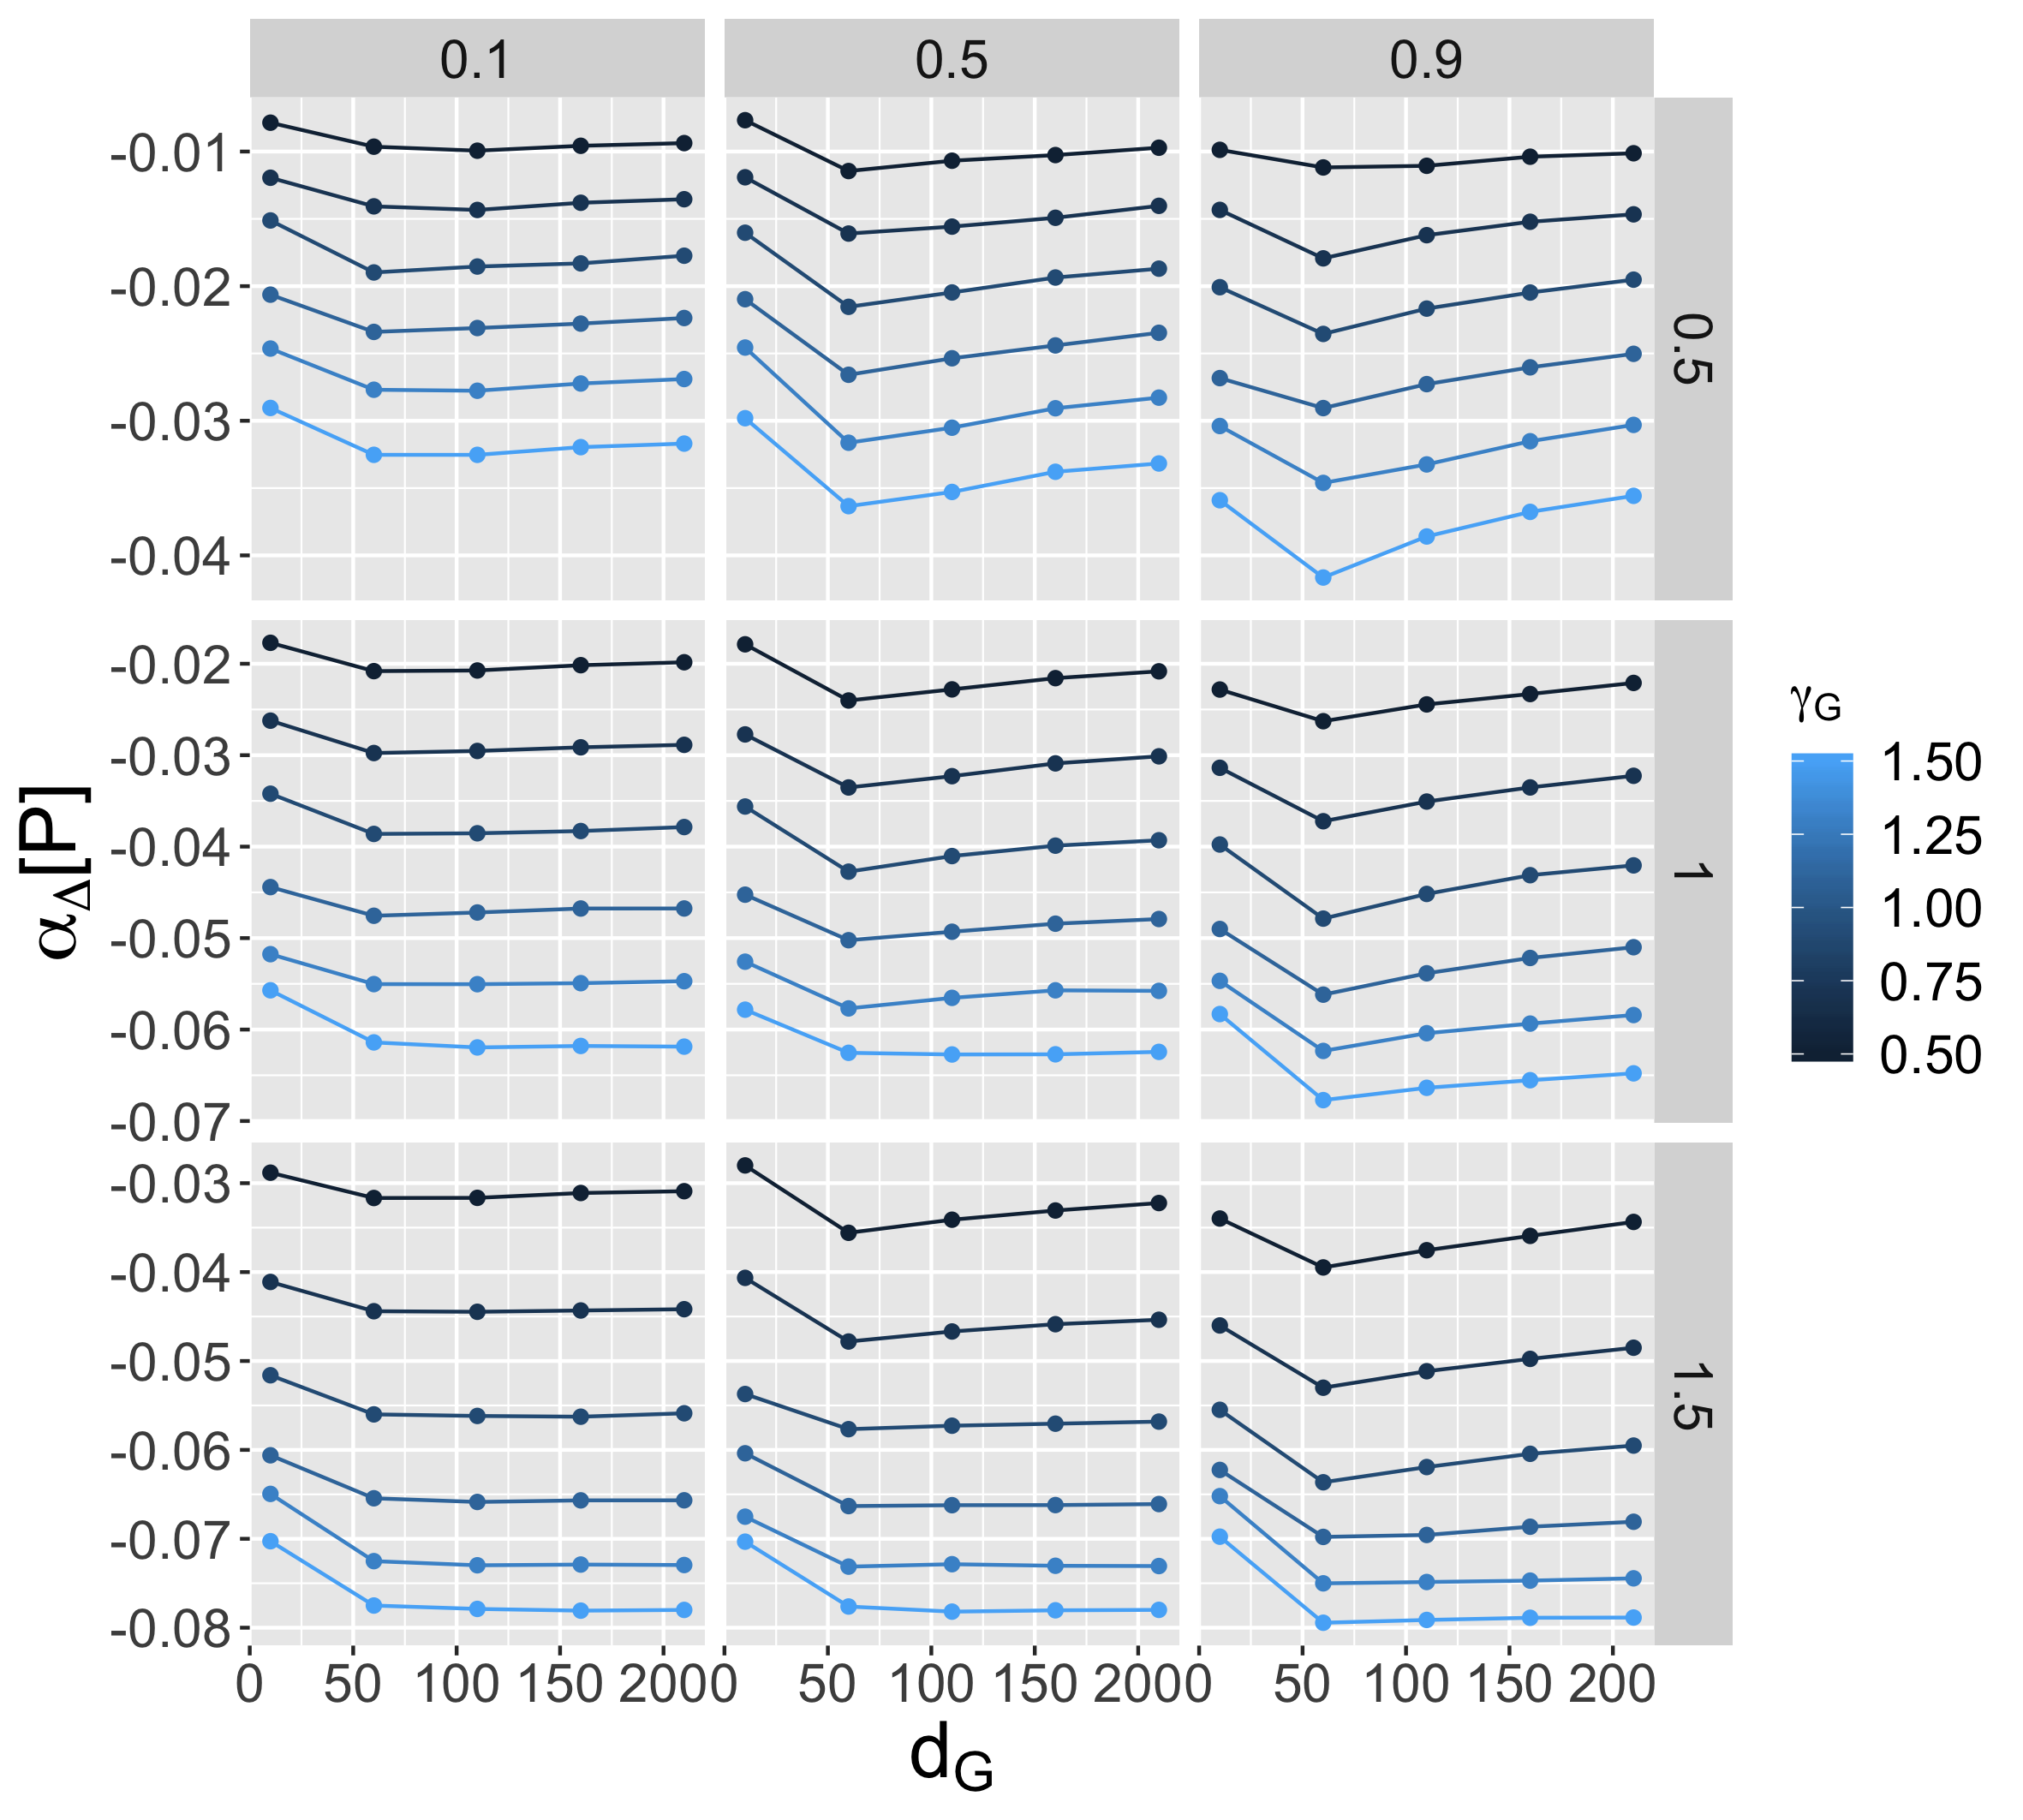
\includegraphics[width=0.48\linewidth]{figures/hierarchiesPopAlpha_nwExp1_wG0_001_xgravityDecay_colgravityGamma_facetsynthRankSize-nwThresholdQuantile.png}
%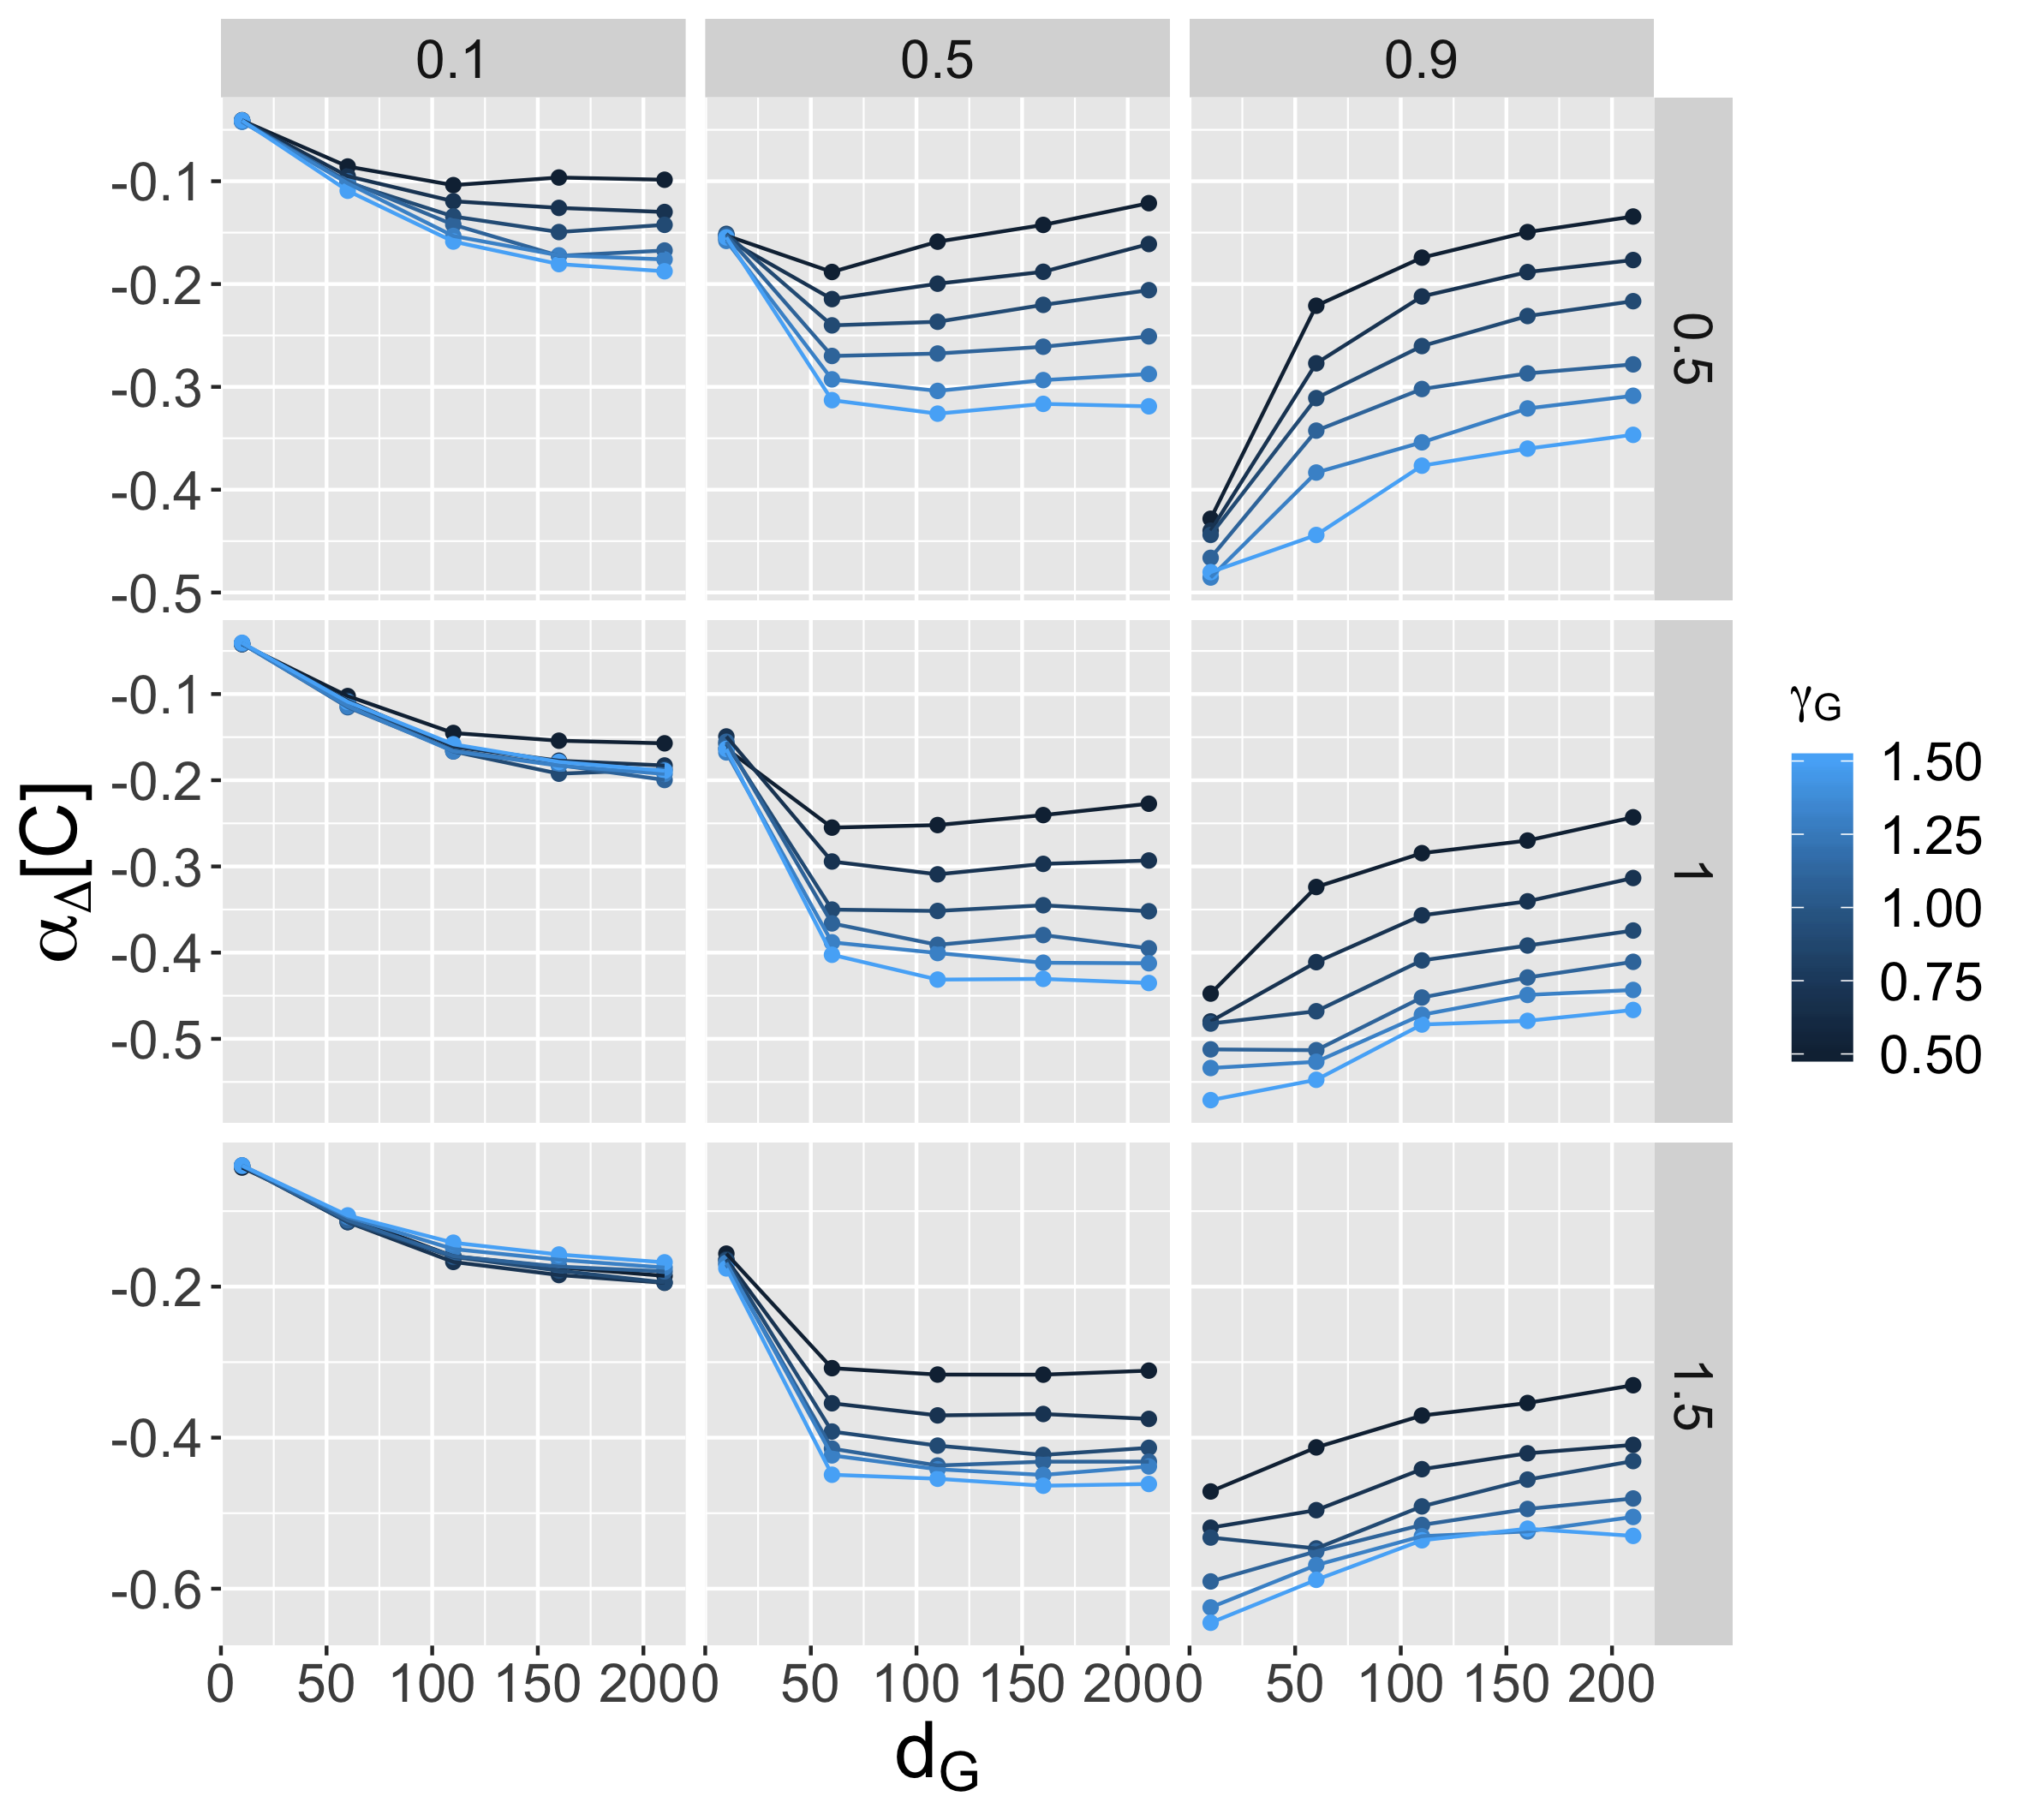
\includegraphics[width=0.48\linewidth]{figures/hierarchiesClosenessAlpha_nwExp1_wG0_001_xgravityDecay_colgravityGamma_facetsynthRankSize-nwThresholdQuantile.png}\\
%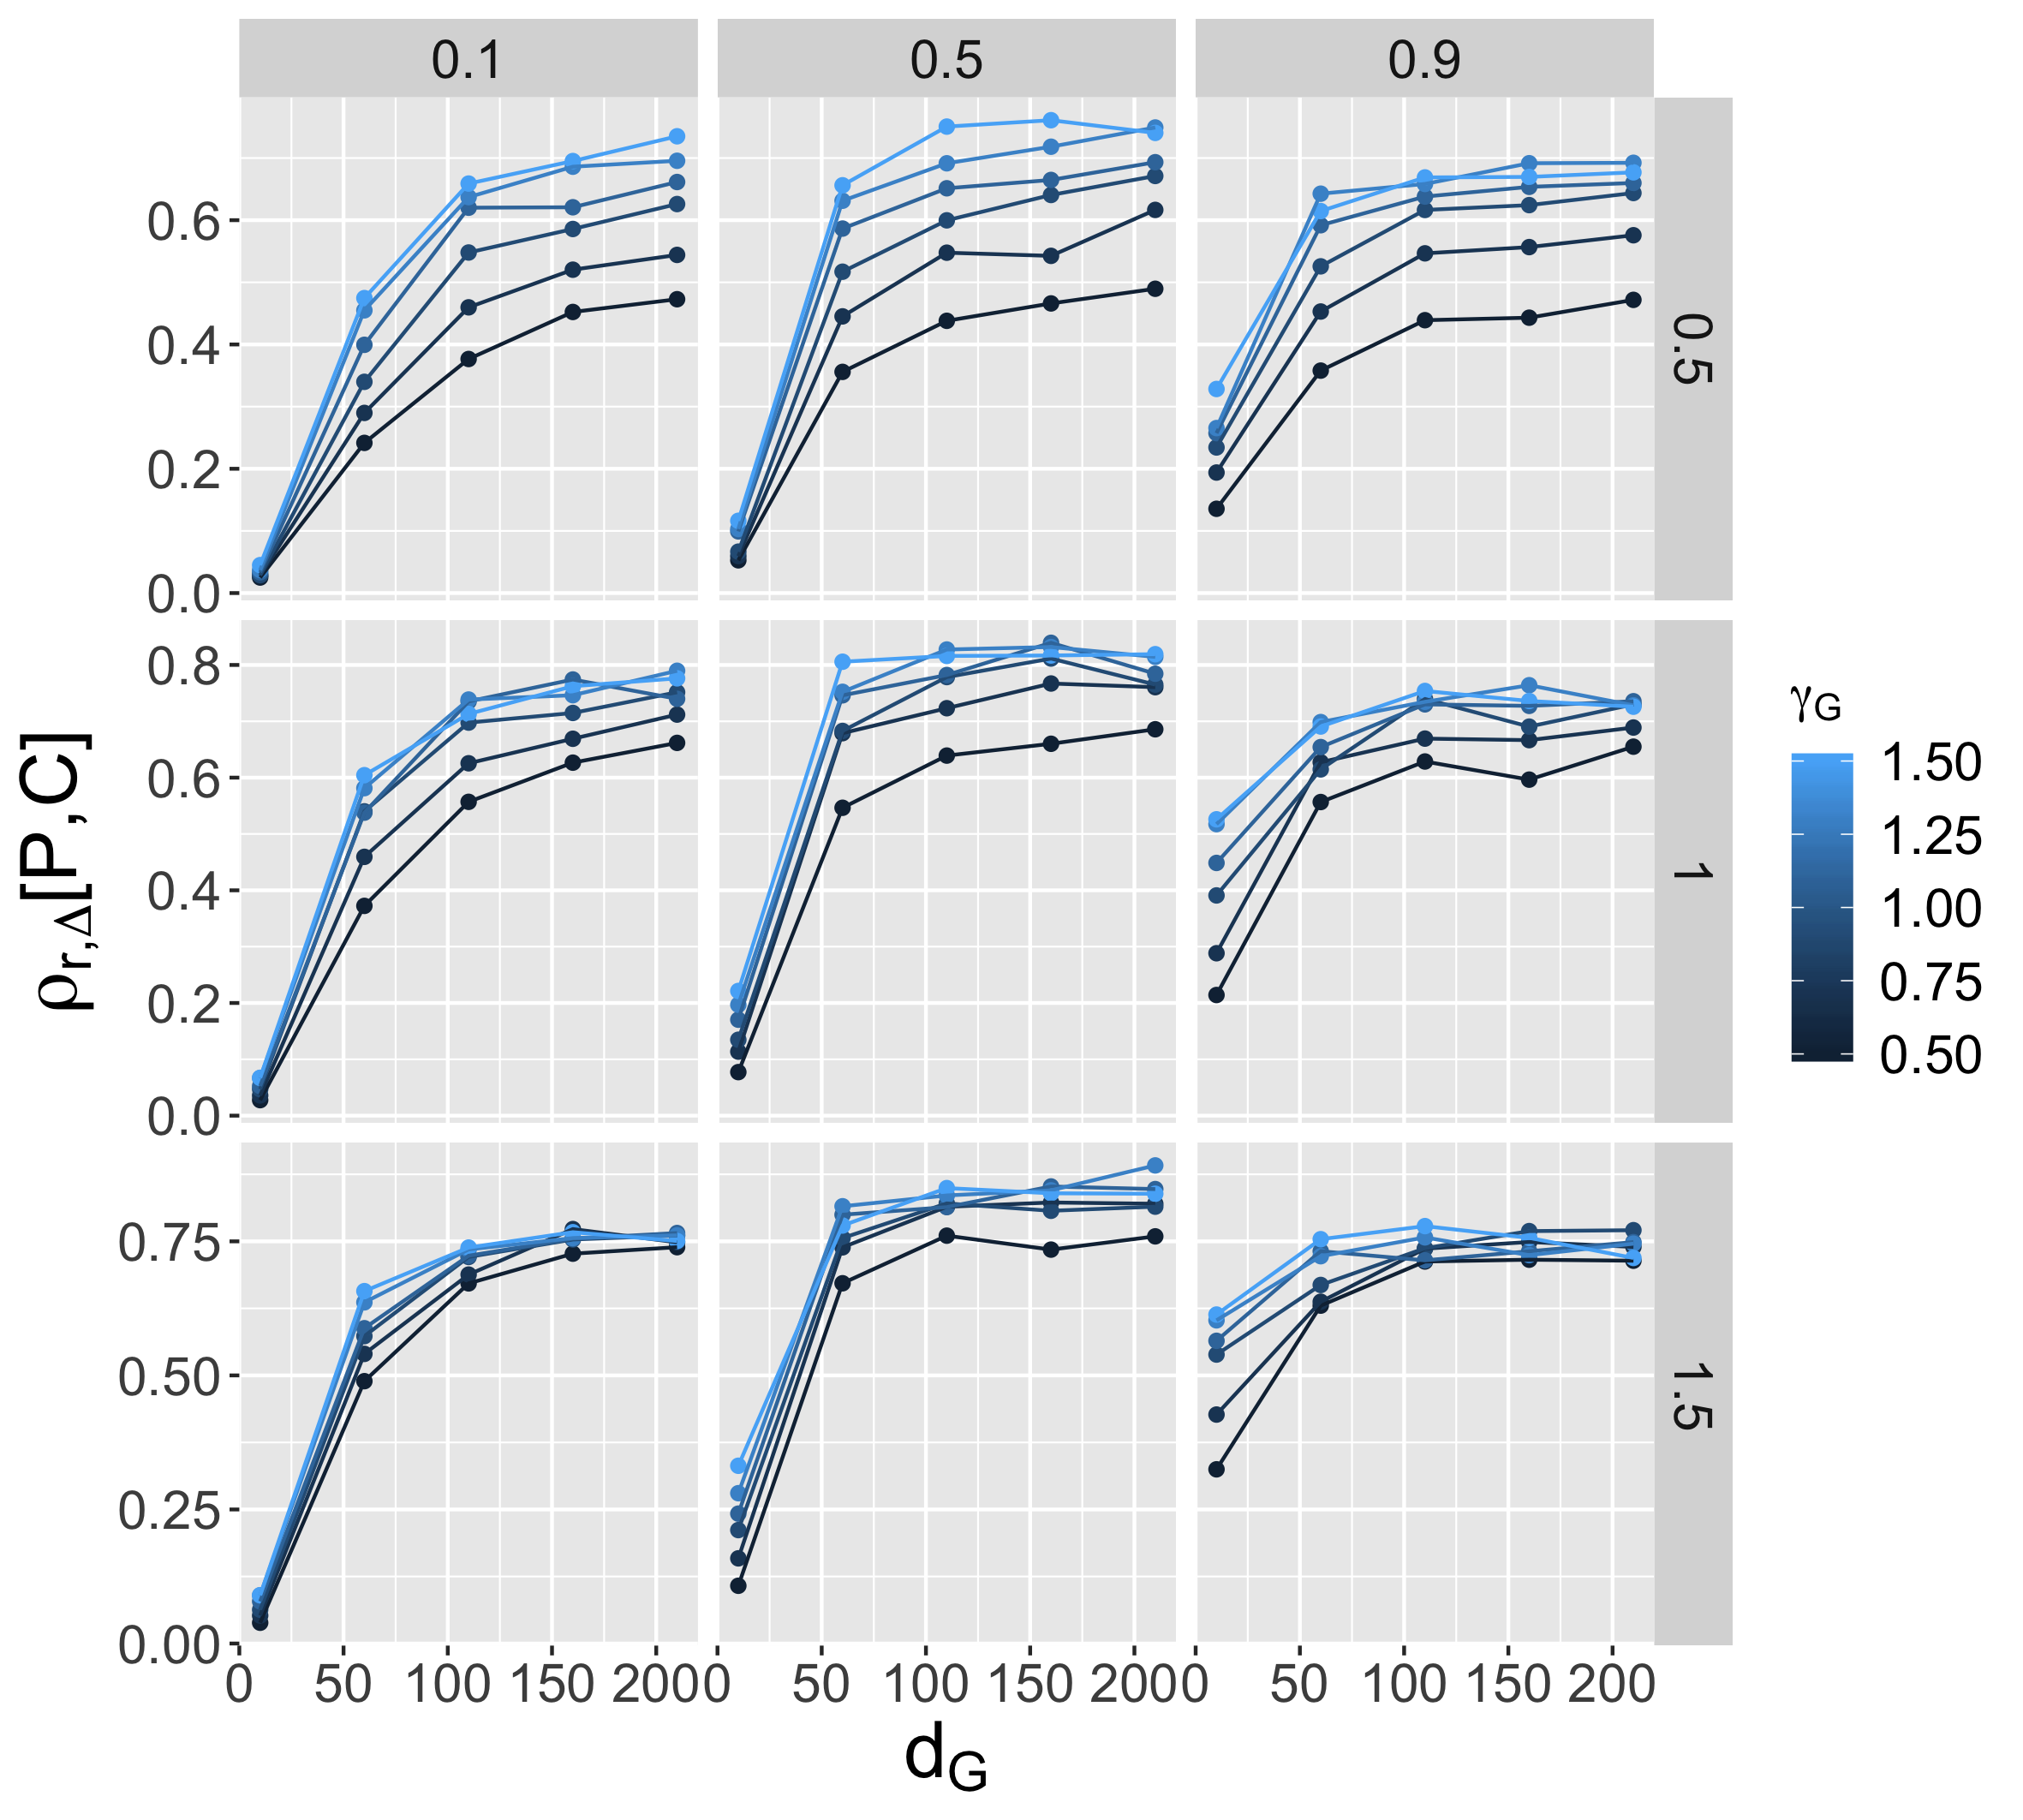
\includegraphics[width=0.48\linewidth]{figures/rankCorrsPopCloseness_nwExp1_wG0_001_xgravityDecay_colgravityGamma_facetsynthRankSize-nwThresholdQuantile.png}
%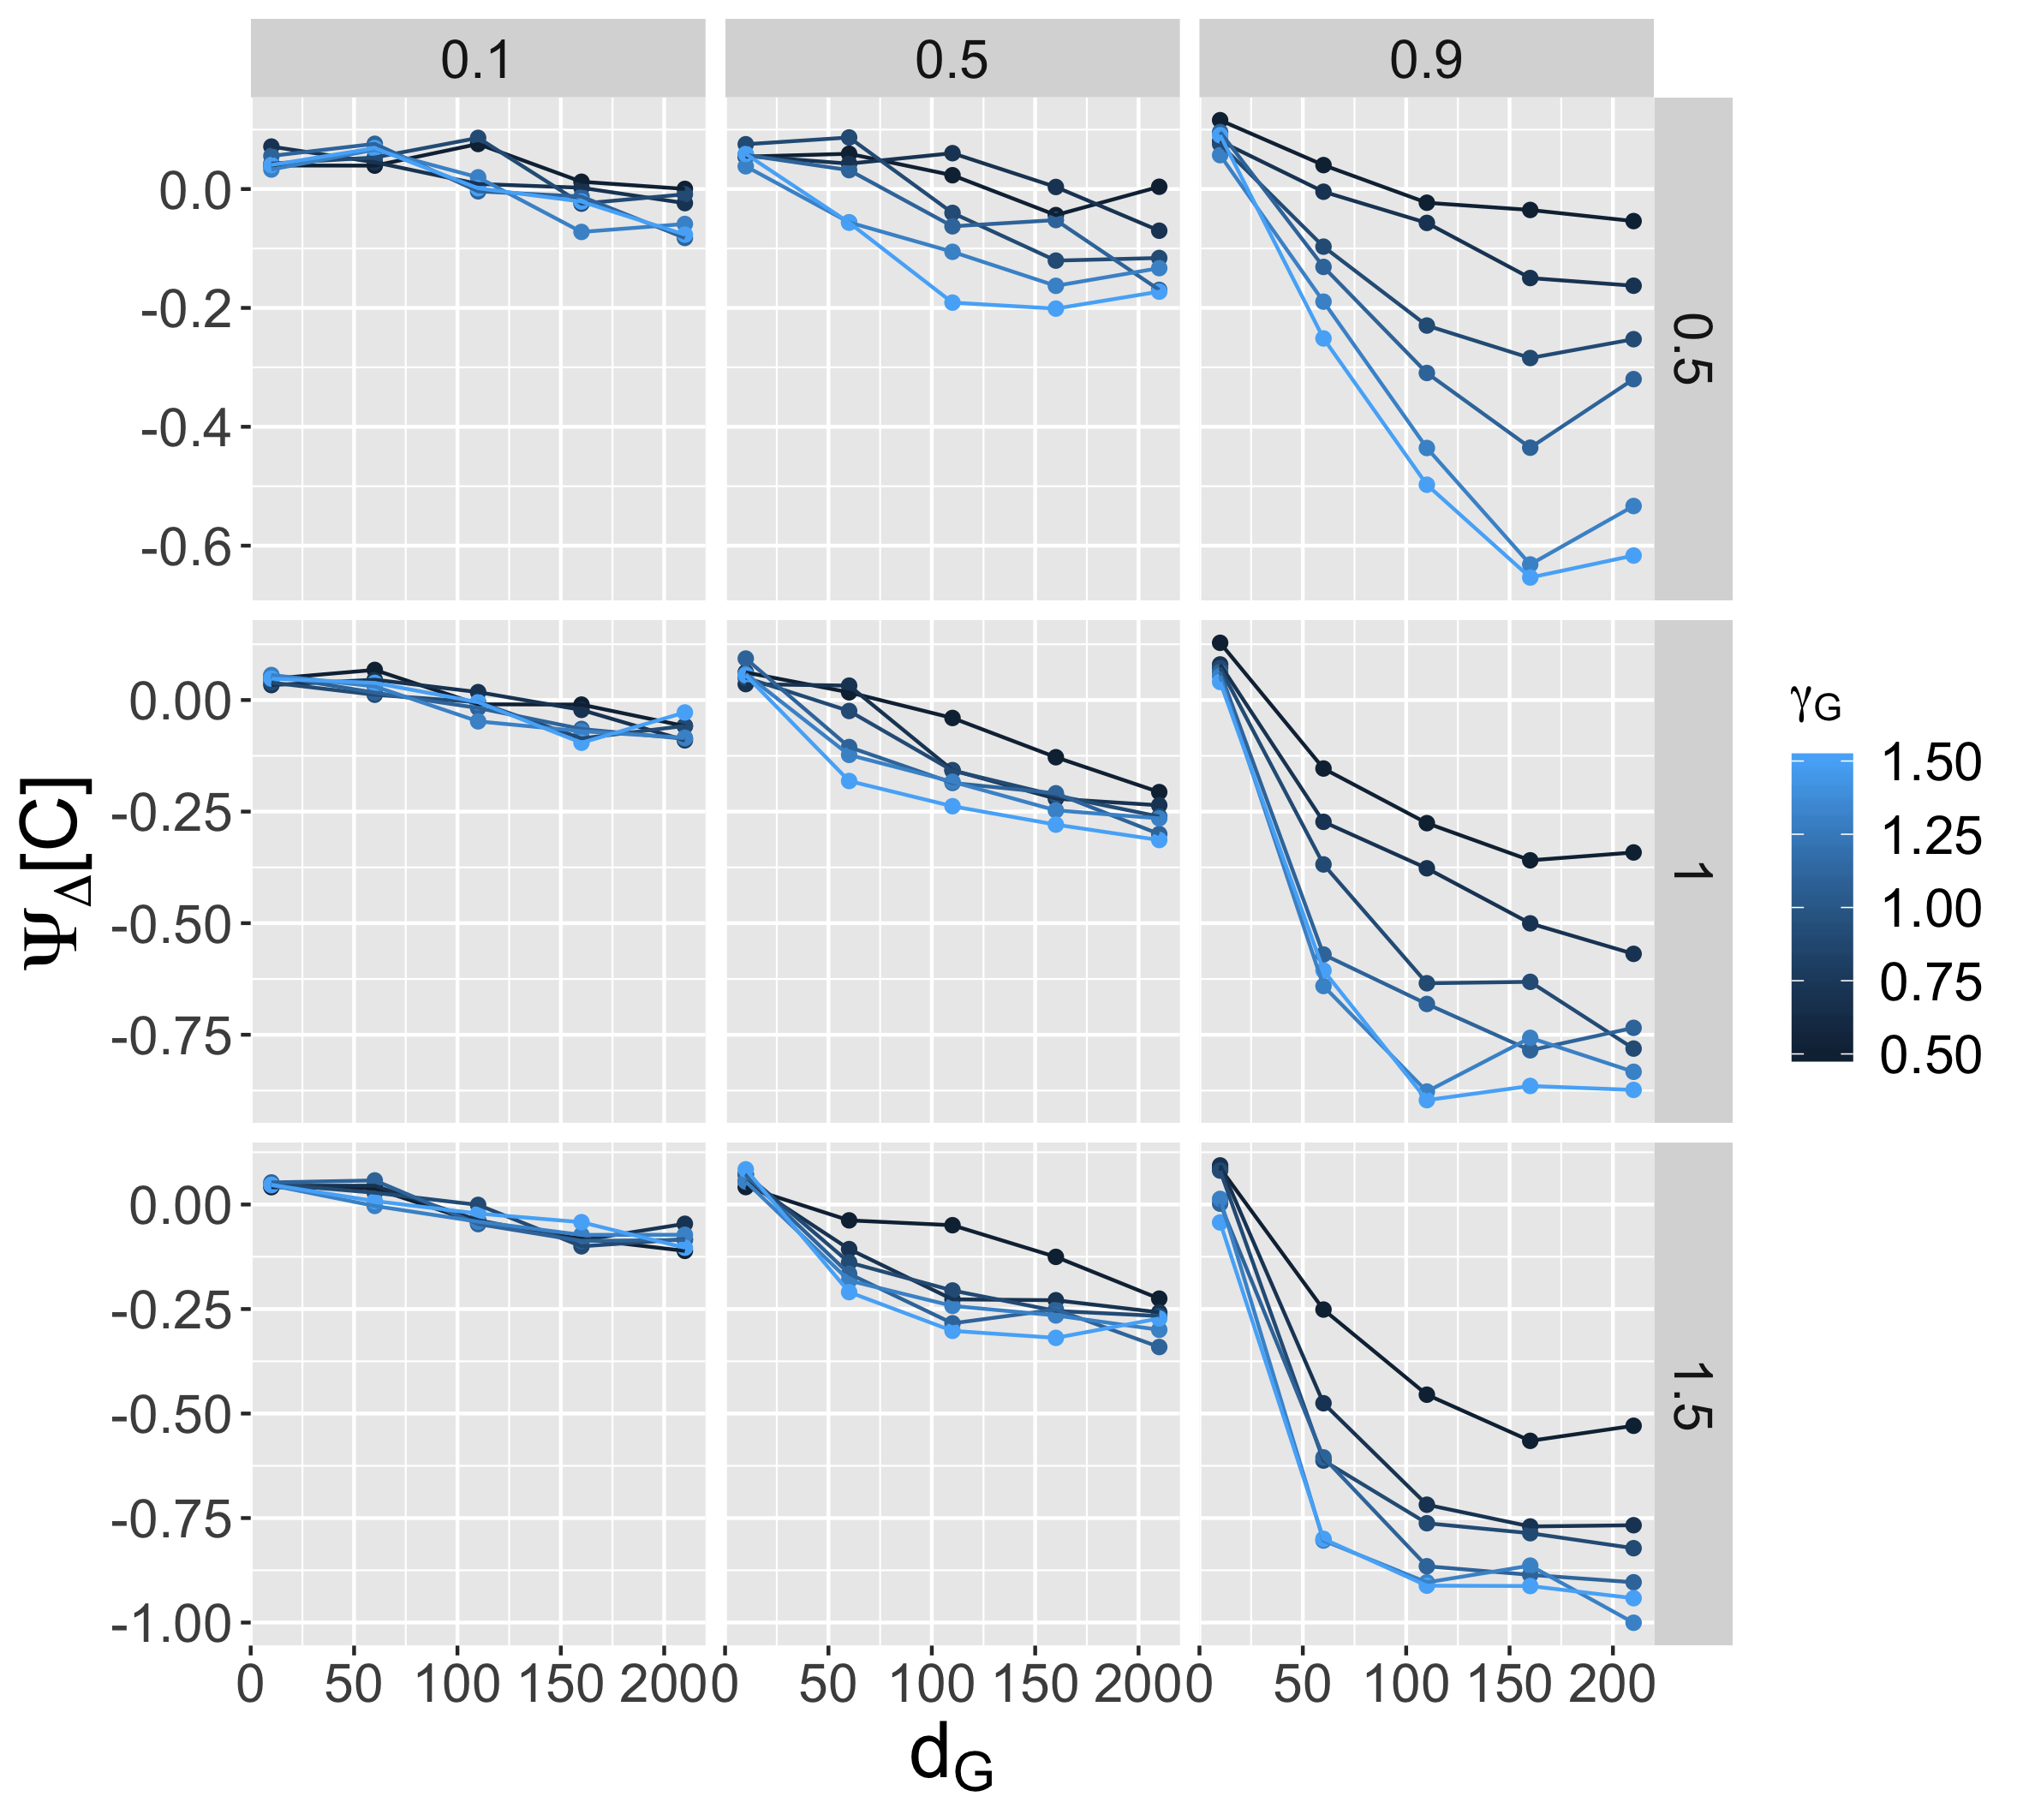
\includegraphics[width=0.48\linewidth]{figures/segHierarchiesClosenessPsi_nwExp1_wG0_001_xgravityDecay_colgravityGamma_facetsynthRankSize-nwThresholdQuantile.png}
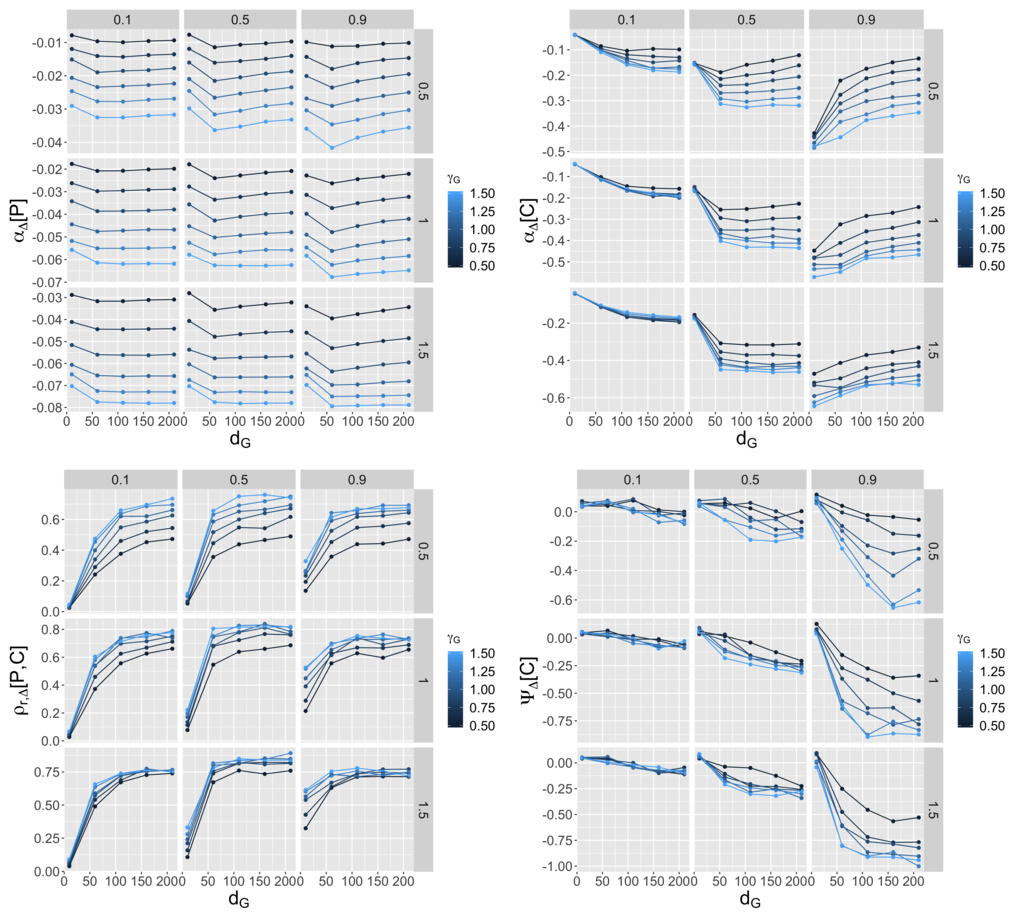
\includegraphics[width=\linewidth]{figures/Fig2.png}
\bpar{
\caption{\textbf{Patterns of hierarchy in the model with a virtual network.} Each indicator is shown as a function of $d_G$ for varying $\gamma_G$ (color), varying $\phi_0^{(q)}$ (columns) and varying $\alpha_S$ (rows). \textit{(Top Left)} Difference in the rank-size exponent for populations between final time and initial time; \textit{(Top Right)} Difference in the rank-size exponent for centralities; \textit{(Bottom Left)} Difference in rank correlation between population and centralities; \textit{(Bottom Right)} Difference in breakpoint of the hierarchy of centralities. \label{fig:gridexplo-virtual}}
}{
\caption{\textbf{Motifs de hiérarchie dans le modèle avec réseau virtuel.} Chaque indicateur est montré comme une fonction de $d_G$ pour $\gamma_G$ variant (couleur), $\phi_0^{(q)}$ variant (colones) et $\alpha_S$ variant (lignes). \textit{(Haut Gauche)} Difference pour l'exposant rang-taille des populations entre instant initial et instant final; \textit{(Haut Droite)} Différence de l'exposant des centralités; \textit{(Bas Gauche)} Différence de la corrélation de rang entre population et centralité; \textit{(Bas Droite)} Différence du point de rupture de la hiérarchie des centralités.\label{fig:gridexplo-virtual}}
}
\end{figure}
%%%%%%%%%%%%%%


\bpar{
The variation of some indicators exhibiting an interesting behavior are shown for the model with the virtual network in Fig.~\ref{fig:gridexplo-virtual}. The evolution of city population hierarchy, captured by $\alpha_{\Delta}\left[P\right] = \alpha \left[P\right](t_f) - \alpha_S$ (top left panel of Fig.~\ref{fig:gridexplo-virtual}), exhibits a low qualitative sensitivity to initial hierarchy $\alpha_S$ (rows), but subplots are translated and a significant quantitative sensitivity is observed: in other words, more hierarchical systems produce more hierarchy, what can be expected in such self-reinforcing processes. Always negative values mean that hierarchy always increases. As a function of gravity decay $d_G$, a systematic absolute decrease is observed for the lowest values: very local interaction mitigate the increase in hierarchy. The gravity interaction hierarchy $\gamma_G$ has a monotonous and expected effect, systematically increasing the hierarchy. Finally, an effect of the co-evolution with network distances which yields non-monotonous effects is worth noticing: when network threshold $\phi_0^{(q)}$ increases, a minimum of $\alpha_{\Delta}\left[P\right]$ is observed for high $\gamma_G$ values and low initial hierarchy. In that context, an intermediate range of spatial interaction will yield more hierarchical systems. As only few links increase their speed with this value of network threshold, it means that long range interactions are no longer amplified by the network. Thus, the evolution of city hierarchies depends on several parameters, in a non-monotonous way when interacting with network processes.
}{
La variation de certains indicateurs présentant un comportement intéressant sont montrés pour le modèle avec réseau virtuel en Fig.~\ref{fig:gridexplo-virtual}. L'évolution de la hiérarchie des populations des villes, capturée par $\alpha_{\Delta}\left[P\right] = \alpha \left[P\right](t_f) - \alpha_S$ (panneau haut gauche de la Fig.~\ref{fig:gridexplo-virtual}), présente une sensibilité qualitative faible à la hiérarchie initiale $\alpha_S$ (lignes), mais les sous-graphes sont translatés et une différence quantitative signifiante est observée: en d'autres termes, des systèmes plus hiérarchiques produisent plus de hiérarchie, ce qui peut être attendu dans de tels processus auto-renforçants. Des valeurs toujours négatives signifient que la hiérarchie augmente toujours. Comme fonction de la distance gravitaire $d_G$, une décroissance absolue systématique est observée pour les valeurs les plus faibles: des interactions très locales limitent l'accroissement de la hiérarchie. La hiérarchie des interactions gravitaires $\gamma_G$ a un effet monotone et attendu, augmentant systématiquement la hiérarchie. Enfin, un effet de la co-évolution avec les distances du réseau qui produit des effets non-monotones est important à noter: quand le seuil de réseau $\phi_0^{(q)}$ s'accroît, un minimum pour $\alpha_{\Delta}\left[P\right]$  est observé pour les fortes valeurs de $\gamma_G$ et les faibles hiérarchies initiales. Dans ce contexte, un portée intermédiaire des interactions spatiales produira des systèmes plus hiérarchiques. Comme seulement peu de liens accroissent leur vitesse avec cette valeur du seuil de réseau, cela signifie que les interactions à longue portée ne sont plus amplifiées par le réseau. Ainsi, l'évolution des hiérarchies des villes dépend de divers paramètres, de façon non-monotone quand elle interagit avec les processus de réseau.
}

\bpar{
Regarding the evolution of network hierarchies $\alpha_{\Delta}\left[C\right]$ (top right panel of Fig.~\ref{fig:gridexplo-virtual}), the most significant effect is the one of network threshold $\phi_0^{(q)}$, which witnesses an inversion of the sense of variation as a function of distance decay $d_G$ when network threshold increases. When all links are allowed to grow their speed, longer span interaction will lead to more hierarchical networks: indeed, the probability for two large cities to interact is then higher, and their flow will be favored in terms of network growth. But when only a few proportion of links improve their travel time while most of them decay, then higher network hierarchies are produced by the most local interactions. In a setting of a scarcity of network investments, taking into account long range interaction gives thus a more balanced network than a local approach, which is kind of counter-intuitive.
}{
En ce qui concerne l'évolution des hiérarchies de réseau $\alpha_{\Delta}\left[C\right]$ (panneau haut droite de la Fig.~\ref{fig:gridexplo-virtual}), l'effet le plus significatif est celui du seuil de réseau $\phi_0^{(q)}$, qui témoigne d'une inversion du sens de variation en fonction de la distance d'interaction $d_G$ quand le seuil de réseau s'accroît. Quant l'ensemble des liens peuvent accroitre leur vitesse, des interactions à plus longue portée produiront des réseaux plus hiérarchiques: en effet, la probabilité pour deux grandes villes d'interagir est alors plus grande, et leur flux sera favorisé en termes de croissance de réseau. Mais quand seulement une petite proportion de liens améliorent leur temps de trajet quand la majorité décroit, alors les plus grandes hiérarchies de réseau sont produites par les interactions les plus locales. Dans un contexte de rareté des investissements de réseau, la prise en compte des interactions de longue portée donne ainsi un réseau plus équilibré qu'une approche locale, ce qui est d'une certaine manière contre-intuitif.
}


\bpar{
The behavior of the rank correlation between population and centrality $\rho_r \left[P, C \right]$ (bottom left panel of Fig.~\ref{fig:gridexplo-virtual}) informs on the co-evolution processes between the territory and the transportation network. Empirically, the better connectivity of larger cities has been suggested by \cite{bretagnolle2003vitesse} as a signature of co-evolution processes. Our results confirm that indeed such co-evolution processes produce a correspondance between city and network hierarchy, as high values of correlations are attained for interaction spans over 100km. The interaction distance furthermore systematically increase the correlation, and local interaction yield a close to zero correlation except for highly initially hierarchic systems with a high network threshold (in which case some very large cities will still construct a local interaction system). The correlation is maximal at an intermediate value of $\phi_0^{(q)}$, which means that the link selection process plays a role in the synchronization between the two hierarchies, and that the co-evolution process captures more than just a self-reinforcement.
}{
Le comportement de la corrélation de range entre population et centralité $\rho_r \left[P, C \right]$ (panneau bas gauche de la Fig.~\ref{fig:gridexplo-virtual}) informe sur les processus de co-évolution entre le territoire et le réseau de transport. D'un point de vue empirique, la meilleure connectivité des grandes villes a été suggéré par \cite{bretagnolle2003vitesse} comme une signature des processus de co-évolution. Nos résultats confirment qu'en effet de tels processus de co-évolution produisent une correspondence entre hiérarchie urbaine et de réseau, comme des fortes valeurs de corrélations sont obtenues pour des distances d'interaction plus grandes que 100km. La distance d'interaction d'autant plus augmente systématiquement la corrélation, et les interactions locales produisent une corrélation proche de zero à l'exception des systèmes initialement très hiérarchiques et avec un haut seuil de réseau (dans quel cas certaine villes parmi les plus grandes construiront toujours un système d'interaction local). La corrélation est maximale à une valeur intermédiaire de $\phi_0^{(q)}$, ce qui signifie que le processus de sélection de lien joue un rôle dans la synchronisation entre les deux hiérarchies, et que les processus de co-évolution capturent plus qu'un simple auto-renforcement.
}

\bpar{
Finally, as we introduced segmented regression as a finer characterization of hierarchical patterns in a system of cities, we observe an interesting behavior for the variation of the breakpoint for centralities $\Psi_{\Delta}\left[C\right]$. The breakpoints always shifts in time to lower values, meaning that the distribution becomes more unequal in time regarding the most dominating links (in the sense that less links are included in the head of the hierarchy). The shift is stronger when interaction distance is larger and network threshold is larger, meaning that favoring less long range links will break the hierarchy in a more uneven way.
}{
Enfin, comme nous avons introduit la regression par segments comme une caractérisation plus fine des motifs hiérarchiques dans un système de villes, nous observons un comportement intéressant pour la variation du point de rupture pour les centralités $\Psi_{\Delta}\left[C\right]$. Les points de ruptures se décalent dans le temps toujours vers des valeurs plus faibles, ce qui signifie que la distribution devient plus inégale dans le temps par rapport aux liens les plus dominants (au sens où moins de liens sont inclus dans la tête de la hiérarchie). Le décalage est plus fort quand la distance d'interaction est plus large et le seuil de réseau est plus large, ce qui signifie que favoriser moins de liens à grande portée induira un changement de la hiérarchie vers une distribution moins homogène.
}



%%%%%%%%%%%%%%
\begin{figure}
%\centering
%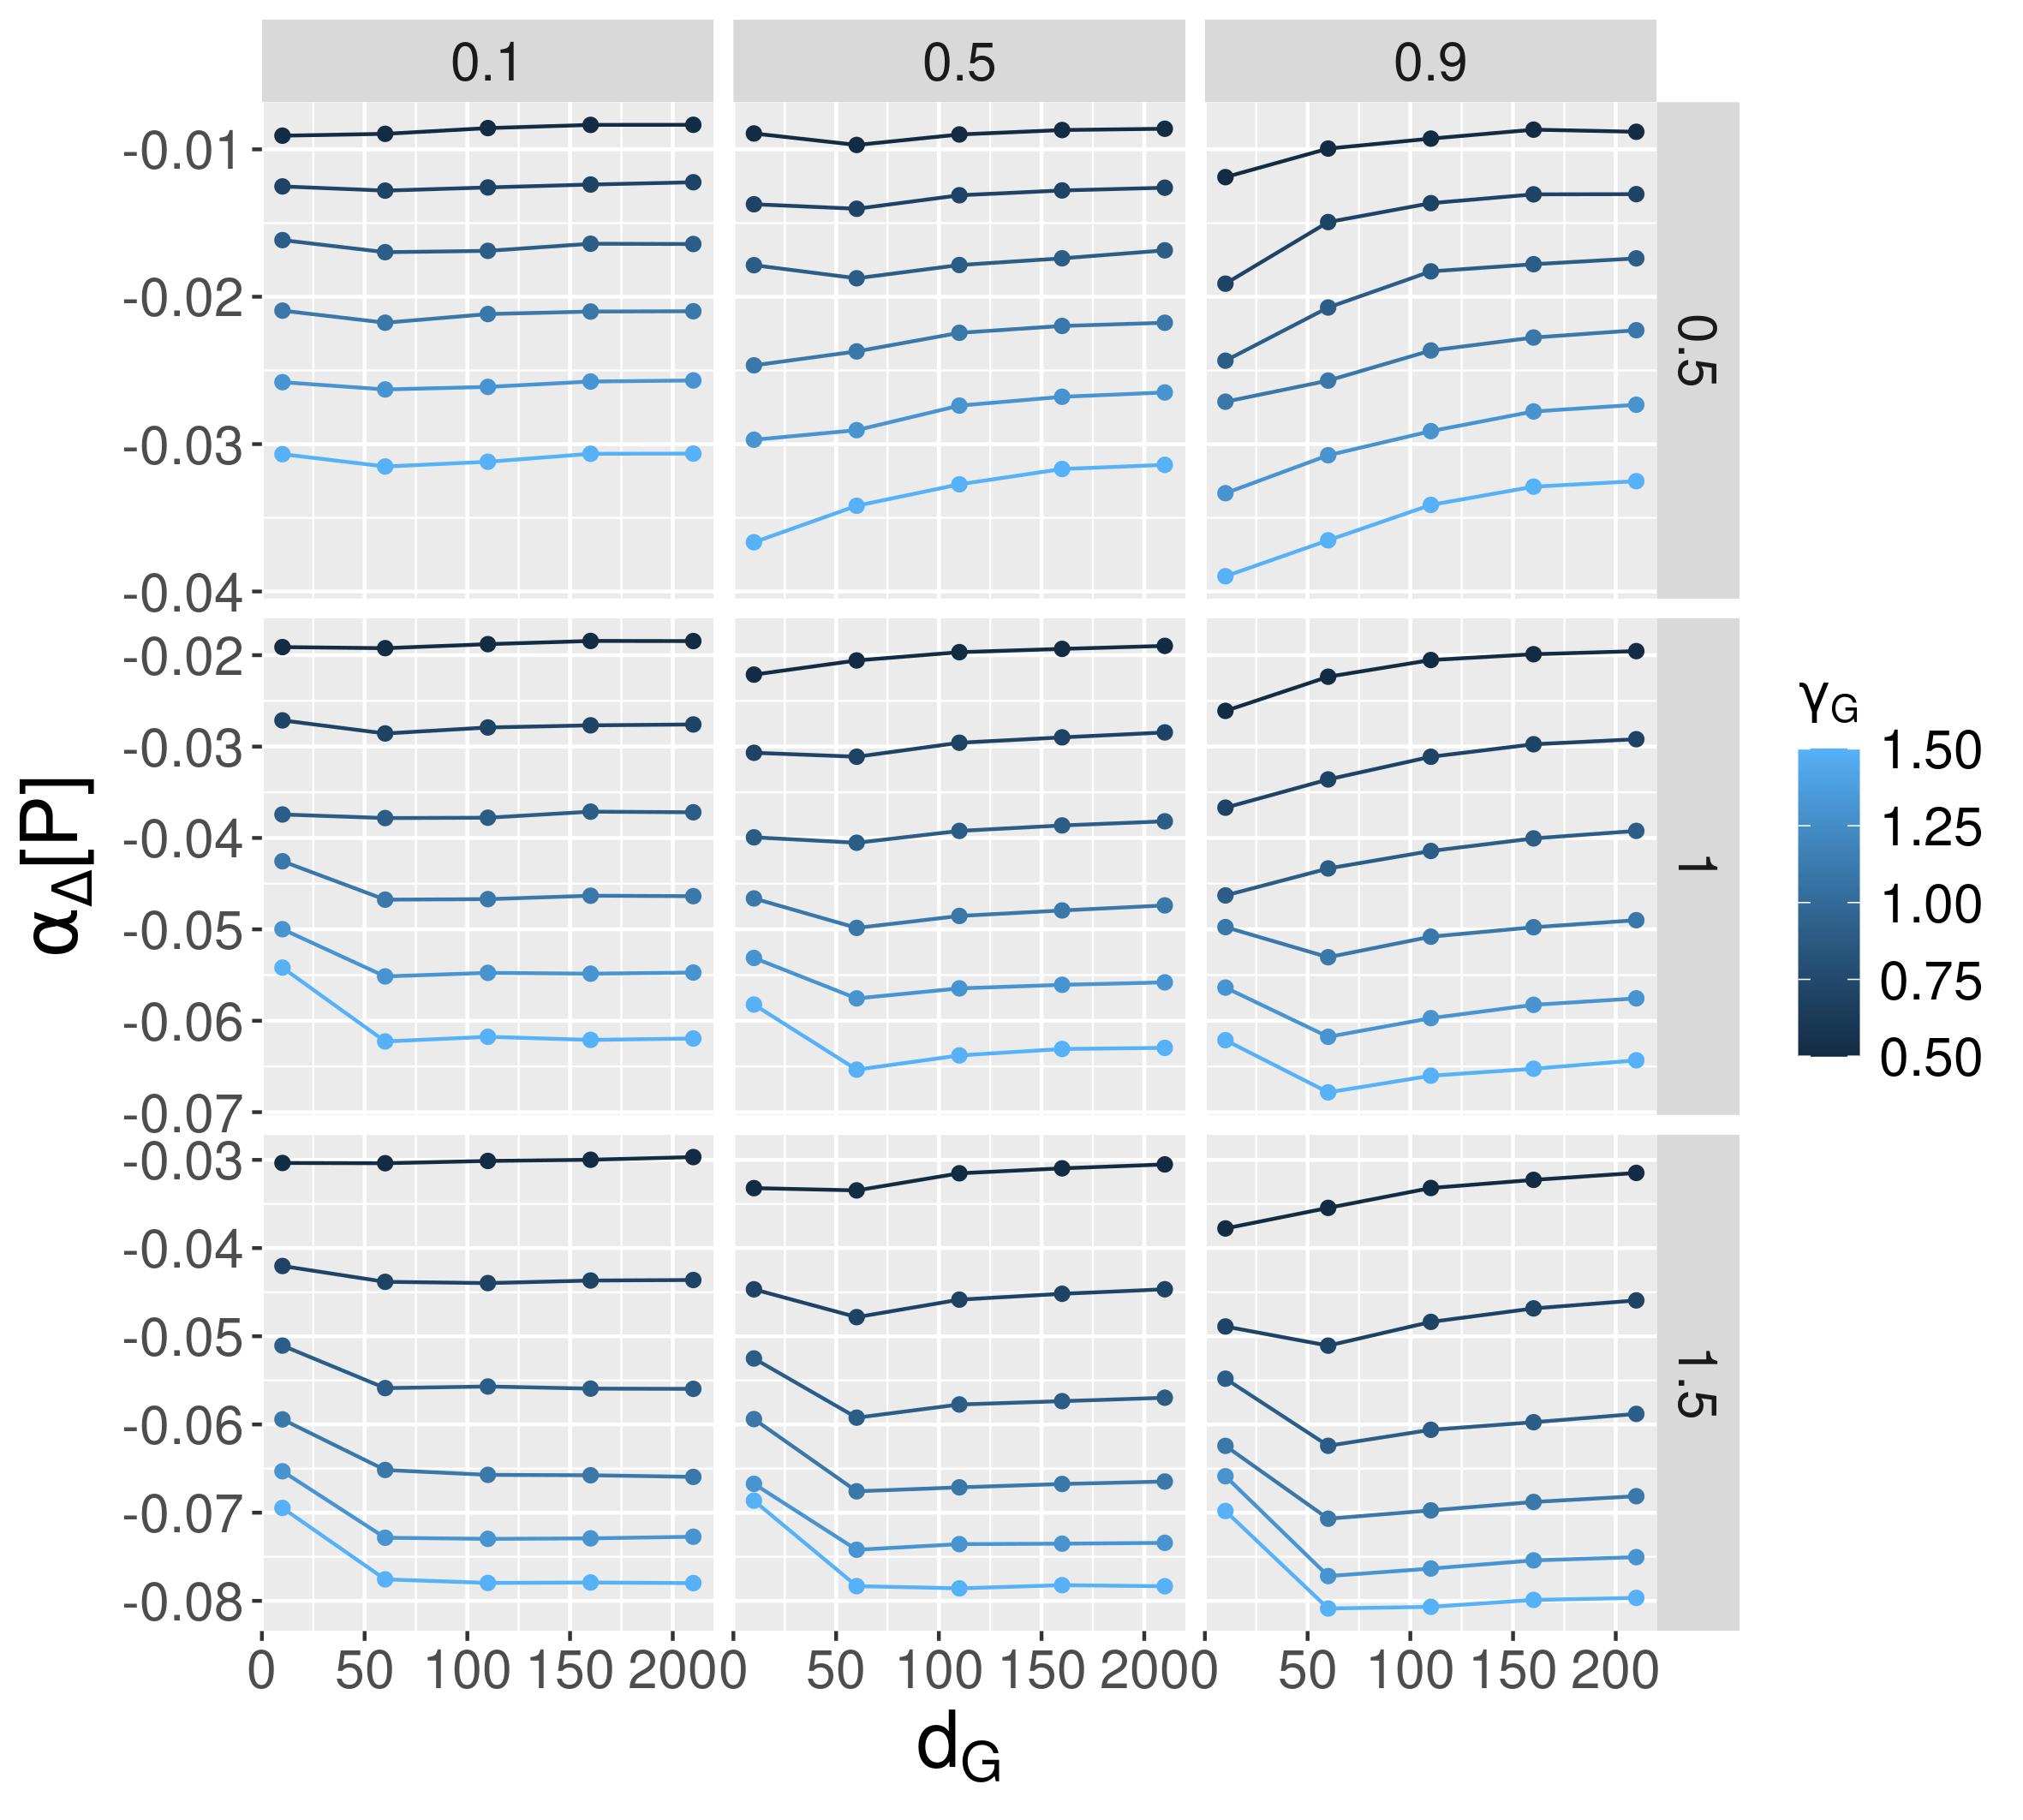
\includegraphics[width=0.48\linewidth]{figures/physical_hierarchiesPopAlpha_nwExp1_wG0_001_xgravityDecay_colgravityGamma_facetsynthRankSize-nwThresholdQuantile.png}
%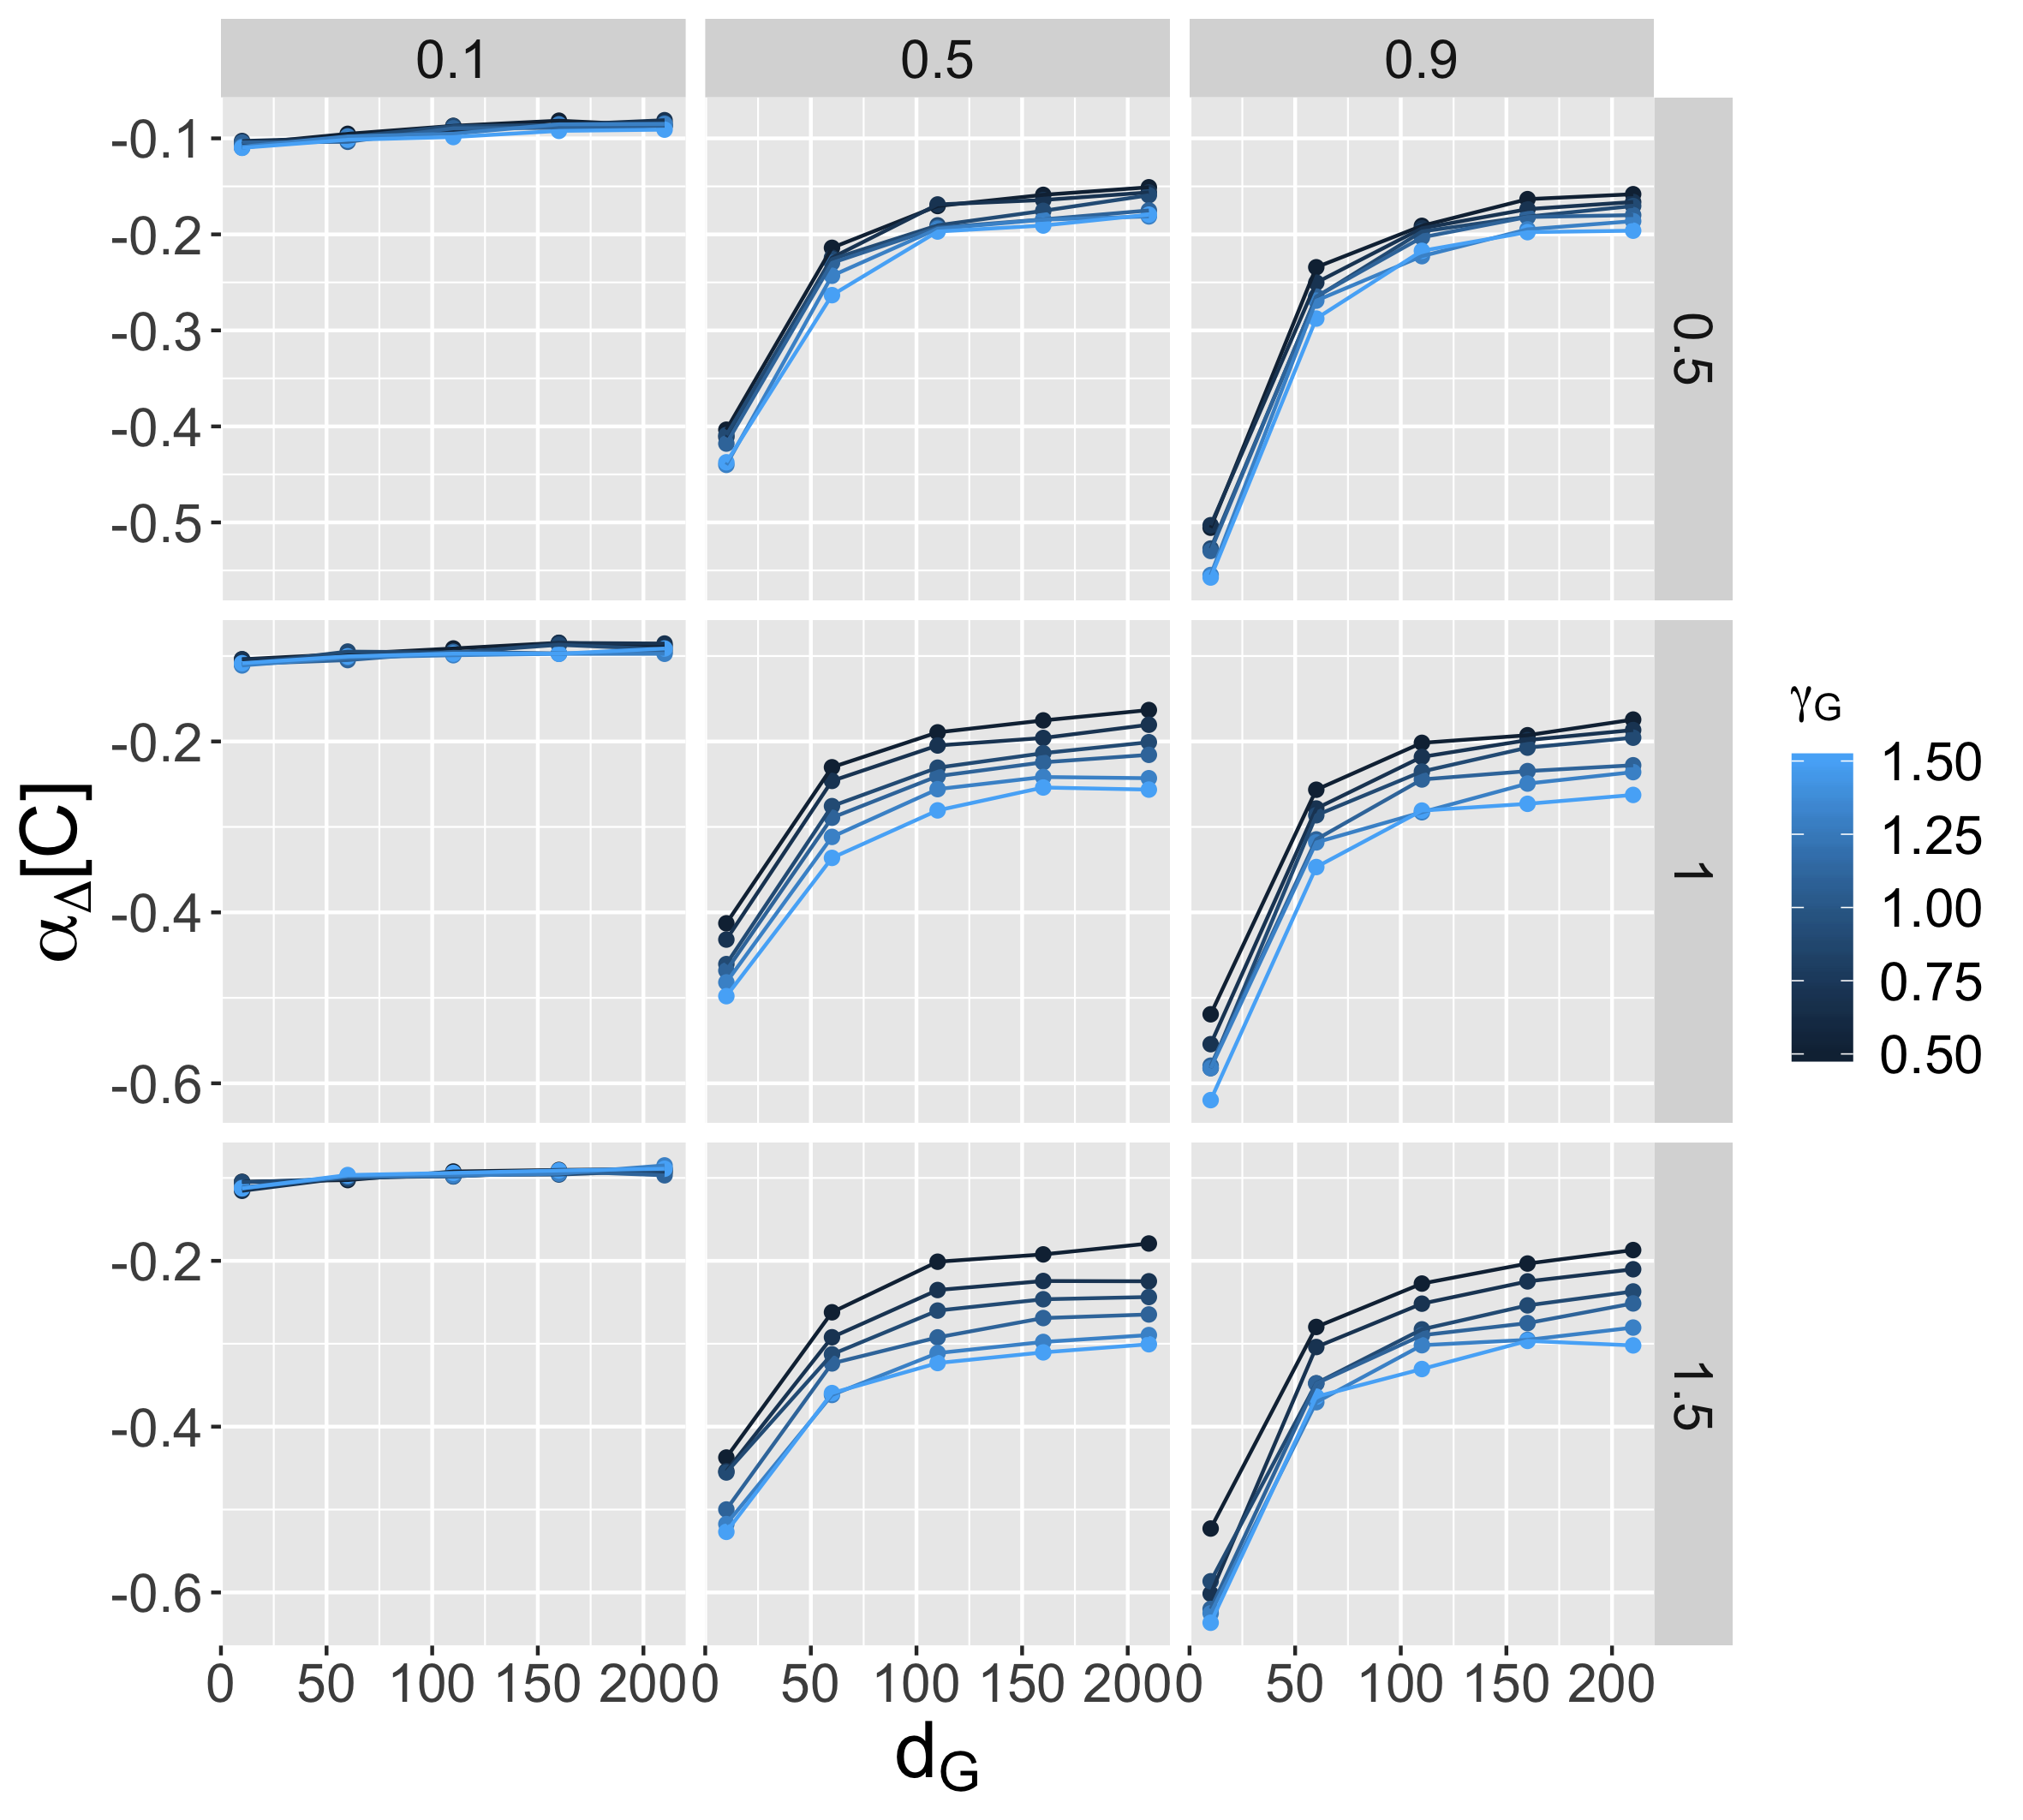
\includegraphics[width=0.48\linewidth]{figures/physical_hierarchiesClosenessAlpha_nwExp1_wG0_001_xgravityDecay_colgravityGamma_facetsynthRankSize-nwThresholdQuantile.png}\\
%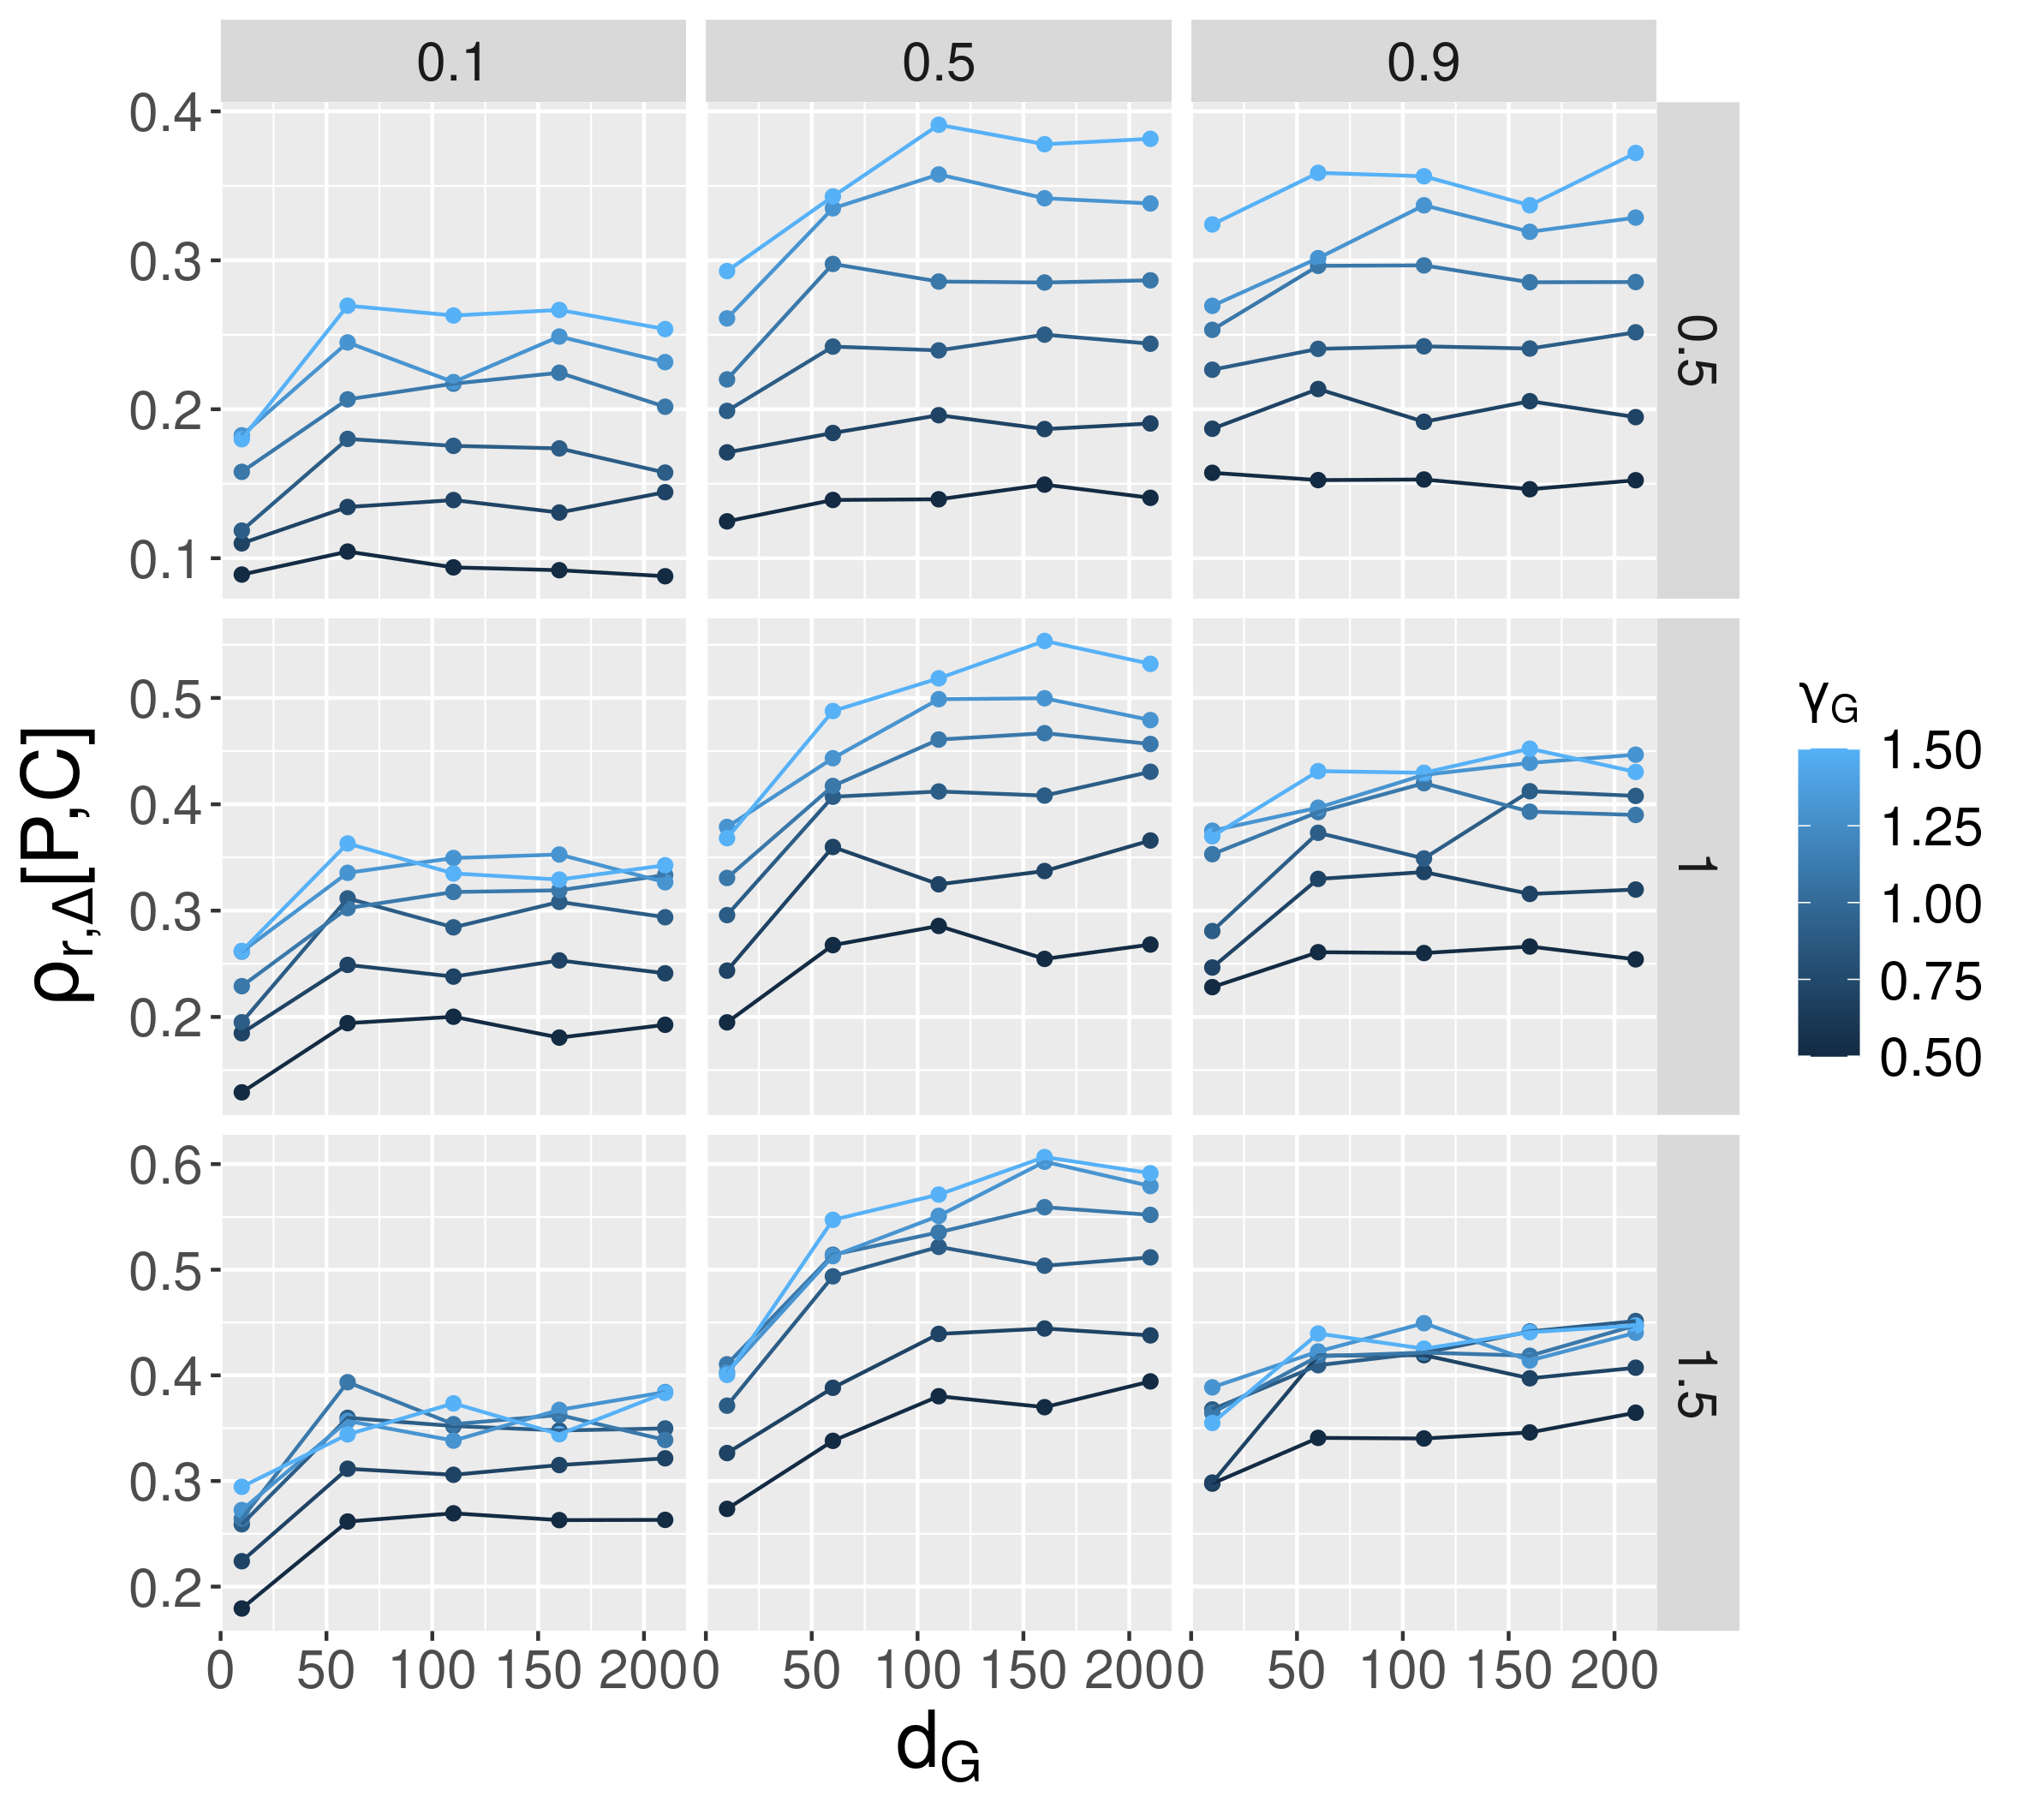
\includegraphics[width=0.48\linewidth]{figures/physical_rankCorrsPopCloseness_nwExp1_wG0_001_xgravityDecay_colgravityGamma_facetsynthRankSize-nwThresholdQuantile.png}
%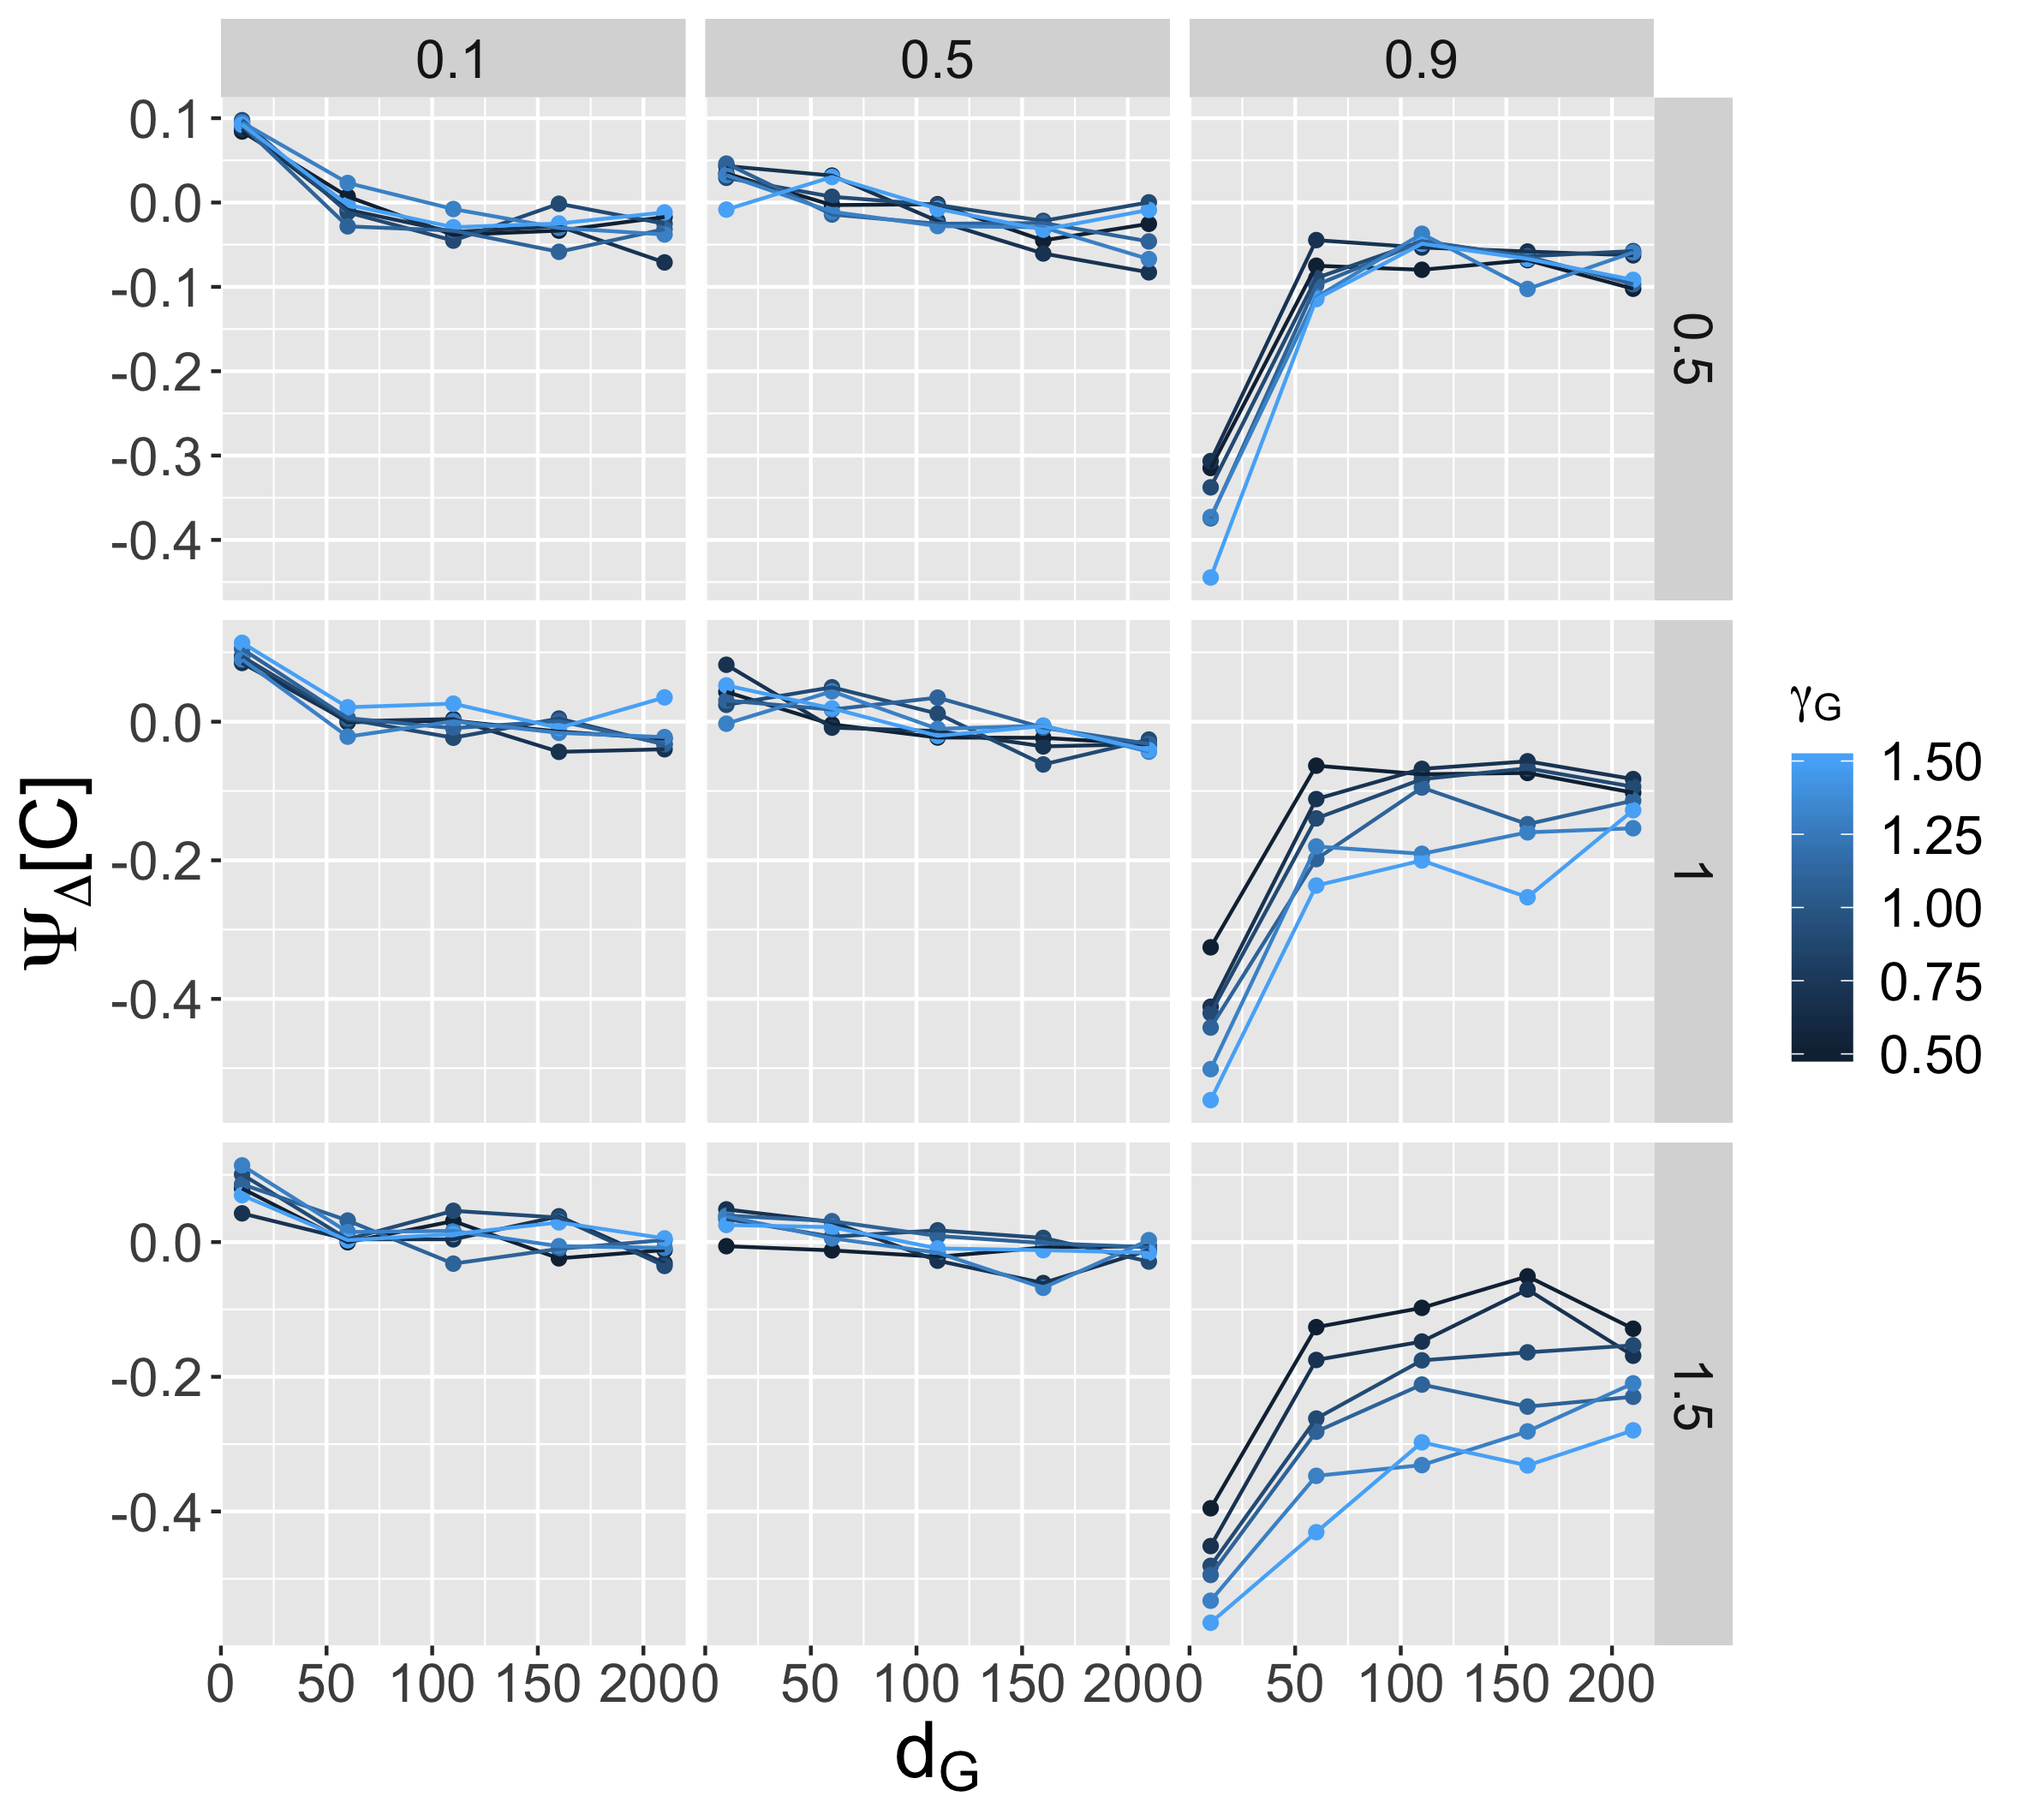
\includegraphics[width=0.48\linewidth]{figures/physical_segHierarchiesClosenessPsi_nwExp1_wG0_001_xgravityDecay_colgravityGamma_facetsynthRankSize-nwThresholdQuantile.png}
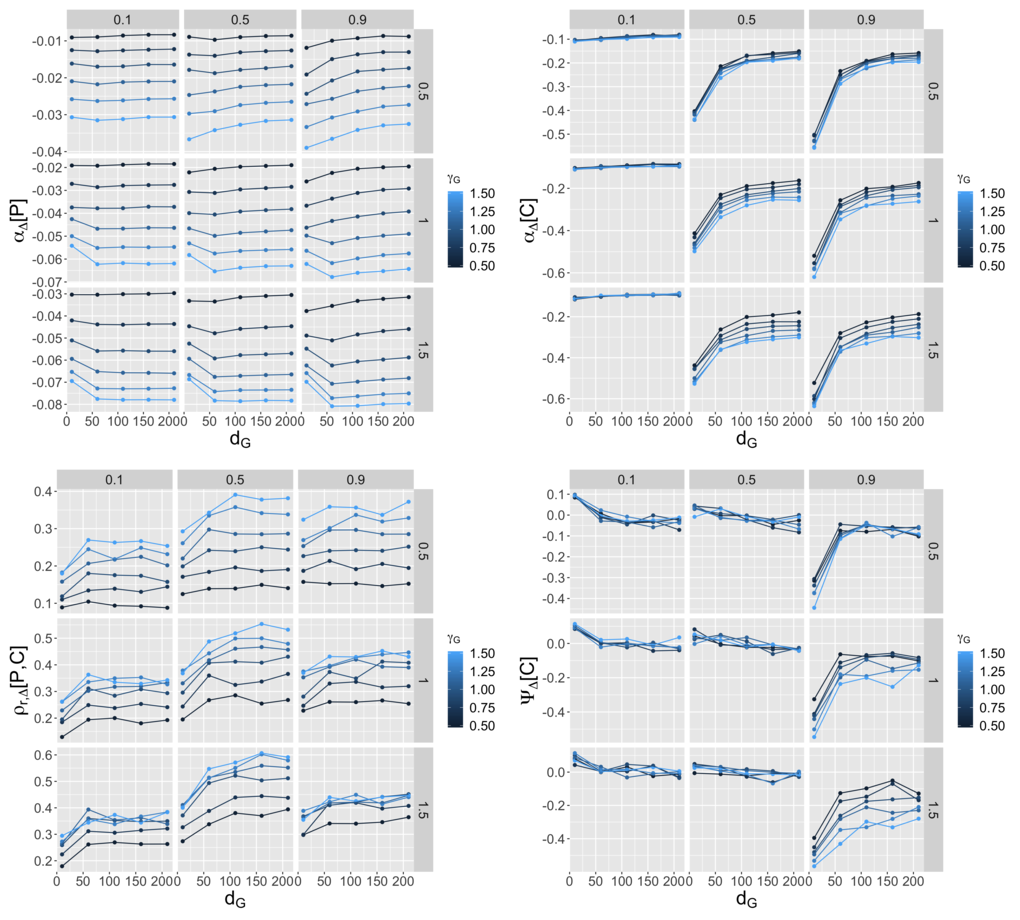
\includegraphics[width=\linewidth]{figures/Fig3.png}
\bpar{
\caption{\textbf{Patterns of hierarchy in the model with a physical network.} With the same design of experiment than in Fig.~\ref{fig:gridexplo-virtual}, each indicator is shown as a function of $d_G$ for varying $\gamma_G$ (color), varying $\phi_0^{(q)}$ (columns) and varying $\alpha_S$ (rows). \textit{(Top Left)} Difference in the rank-size exponent for populations between final time and initial time; \textit{(Top Right)} Difference in the rank-size exponent for centralities; \textit{(Bottom Left)} Difference in rank correlation between population and centralities; \textit{(Bottom Right)} Difference in breakpoint of the hierarchy of centralities.\label{fig:gridexplo-physical}}
}{
\caption{\textbf{Motifs de hiérarchie dans le modèle avec réseau physique.} Avec le même plan d'expérience qu'en Fig.~\ref{fig:gridexplo-virtual}, chaque indicateur est montré comme fonction de $d_G$ pour $\gamma_G$ variant (couleur), $\phi_0^{(q)}$ variant (colones) et $\alpha_S$ variant (lignes) \textit{(Haut Gauche)} Différence de l'exposant rang-taille des populations entre instant initial et instant final; \textit{(Haut Droite)} Différence dans l'exposant rang-taille des centralités; \textit{(Bas Gauche)} Différence de la corrélation de rang entre population et centralité; \textit{(Bas Droite)} Différence du point de rupture des centralités.\label{fig:gridexplo-physical}}
}
\end{figure}
%%%%%%%%%%%%%%


\bpar{
Our second experiment to study patterns of hierarchy is the same exact Design of Experiment than the previous one, but with the physical network. We show in Fig.~\ref{fig:gridexplo-physical} the same indicators for the same parameter space. The discrepancy between the two behaviors is particularly relevant from a thematic point of view, as it reveals the role of spatializing and assigning network flows, even in such as case where no congestion is included. Some patterns are similar, but some important differences can be observed. Globally, the behavior of population hierarchy, rank correlation, and centrality hierarchy breakpoint, are qualitatively similar. The minimum which existed for population hierarchies at short range interactions mostly disappears (although still slightly present for $\gamma_G = 1.5$, $\phi_0^{(q)} = 0.9$ and $\alpha_S = 1$): spatializing the network removes some output complexity in that case. Rank correlations (bottom panel of Fig.~\ref{fig:gridexplo-physical}), i.e. the correspondance between population and centrality hierarchies, is still growing as a function of $d_G$ and exhibits a maximum at the intermediate value $\phi_0^{(q)}$. However, the effect of interaction hierarchy $\gamma_G$ is much more impactful in this case: more uniform interactions (low $\gamma_G$) lead to a much smaller correlation. This means that the approximation of using a virtual network accurately captures the hierarchy correspondance in physical networks for flows with a superlinear scaling exponent: depending on the type of activities generating flows, spatial structure of the network is more or less important.
}{
Notre seconde expérience pour étudier les motifs de hiérarchie est exactement le même plan d'expérience que précédemment, mais pour le réseau physique. Nous montrons en Fig.~\ref{fig:gridexplo-physical} les mêmes indicateurs pour le même espace de paramètres. Les divergences entre les deux comportements sont particulièrement intéressantes d'un point de vue thématique, puisque elles révèlent le rôle de la spatialisation et de la distribution des flux de réseau, même dans un tel cas où la congestion n'est pas incluse. Certains motifs sont similaires, mais des différences importantes peuvent être observée. Globalement, le comportement le la hiérarchie des populations, de la corrélation de rang, et du point de rupture de la centralité des hiérarchies, sont qualitativement similaires. Le minimum qui existait pour les hiérarchies des populations aux courtes distances d'interaction disparait principalement (même s'il est partiellement visible pour  $\gamma_G = 1.5$, $\phi_0^{(q)} = 0.9$ et $\alpha_S = 1$): la spatialisation du réseau supprime une certaine complexité des sorties dans ce cas. Les corrélations de rang (panneau bas gauche de la Fig.~\ref{fig:gridexplo-physical}), i.e. la correspondence entre hiérarchie des populations et des centralités, est toujours croissante en fonction de $d_G$ et présente un maximum à la valeur intermédiaire $\phi_0^{(q)}$. Cependant, l'effet de la hiérarchie des interactions $\gamma_G$ a bien plus d'impact dans ce cas: des interactions plus uniformes (faible $\gamma_G$) conduisent à une corrélation bien plus faible. Cela signifie que l'approximation d'utiliser un réseau virtuel capture fidèlement la correspondence de hiérarchie dans les réseaux physiques pour les flux avec un exposant d'échelle superlinéaire: selon le type des activités générant les flux, la structure spatiale du réseau est plus ou moins importante.
}


\bpar{
The hierarchy of centralities also behave quite differently when switching to a physical network (top right panel of Fig.~\ref{fig:gridexplo-physical}). It is in that case roughly insensitive to any parameter when all links are growing ($\phi_0^{(q)} = 0.1$), and always grows as a function of distance decay $d_G$: longer range interactions diffuse through most network links and yield less inequality between their speeds. Increasing the hierarchy of interactions still increases the hierarchy of centralities but the effect is less strong. In a nutshell, constraining spatially the links and making them share flows through the assignment procedure restricts the degrees of freedom their speed dynamics have.
}{
La hiérarchie des centralités se comporte aussi assez différemment lors du passage à un réseau physique (panneau haut droite de la Fig.~\ref{fig:gridexplo-physical}). Elle est dans ce cas approximativement insensible à aucun paramètre quand tous les liens croissent ($\phi_0^{(q)} = 0.1$), et est toujours croissante comme fonction de la distance d'interaction $d_G$: des interactions à plus longue portée se diffusent dans la plupart des liens du réseau et produisent moins d'inégalité entre leurs vitesses. L'accroissement de la hiérarchie des interactions augmente toujours la hiérarchie des centralités mais l'effet est moins fort. En résumé, la contrainte spatiale des liens et le fait qu'ils partagent les flux par la procédure de distribution restreint les degrés de liberté que leur dynamiques de vitesses ont.
}



\bpar{
\subsection{Hierarchy regimes}
}{
\subsection{Régimes de hiérarchie}
}

% - PSE targeted on different regimes (dynamical ?) of hierarchy => piecewise linear fitting? 
% => simple three dimensional pattern: alpha_P, alpha_C, rho_r [P, C]

% we use Delta alpha: for population controls on the imposed initial hierarchy (how the model can go beyond the initial hierarchy constraint); for closeness, comparability and given the distribution (only dep on geometry! - similar)


%%%%%%%%%%%%%%
\begin{figure}
	%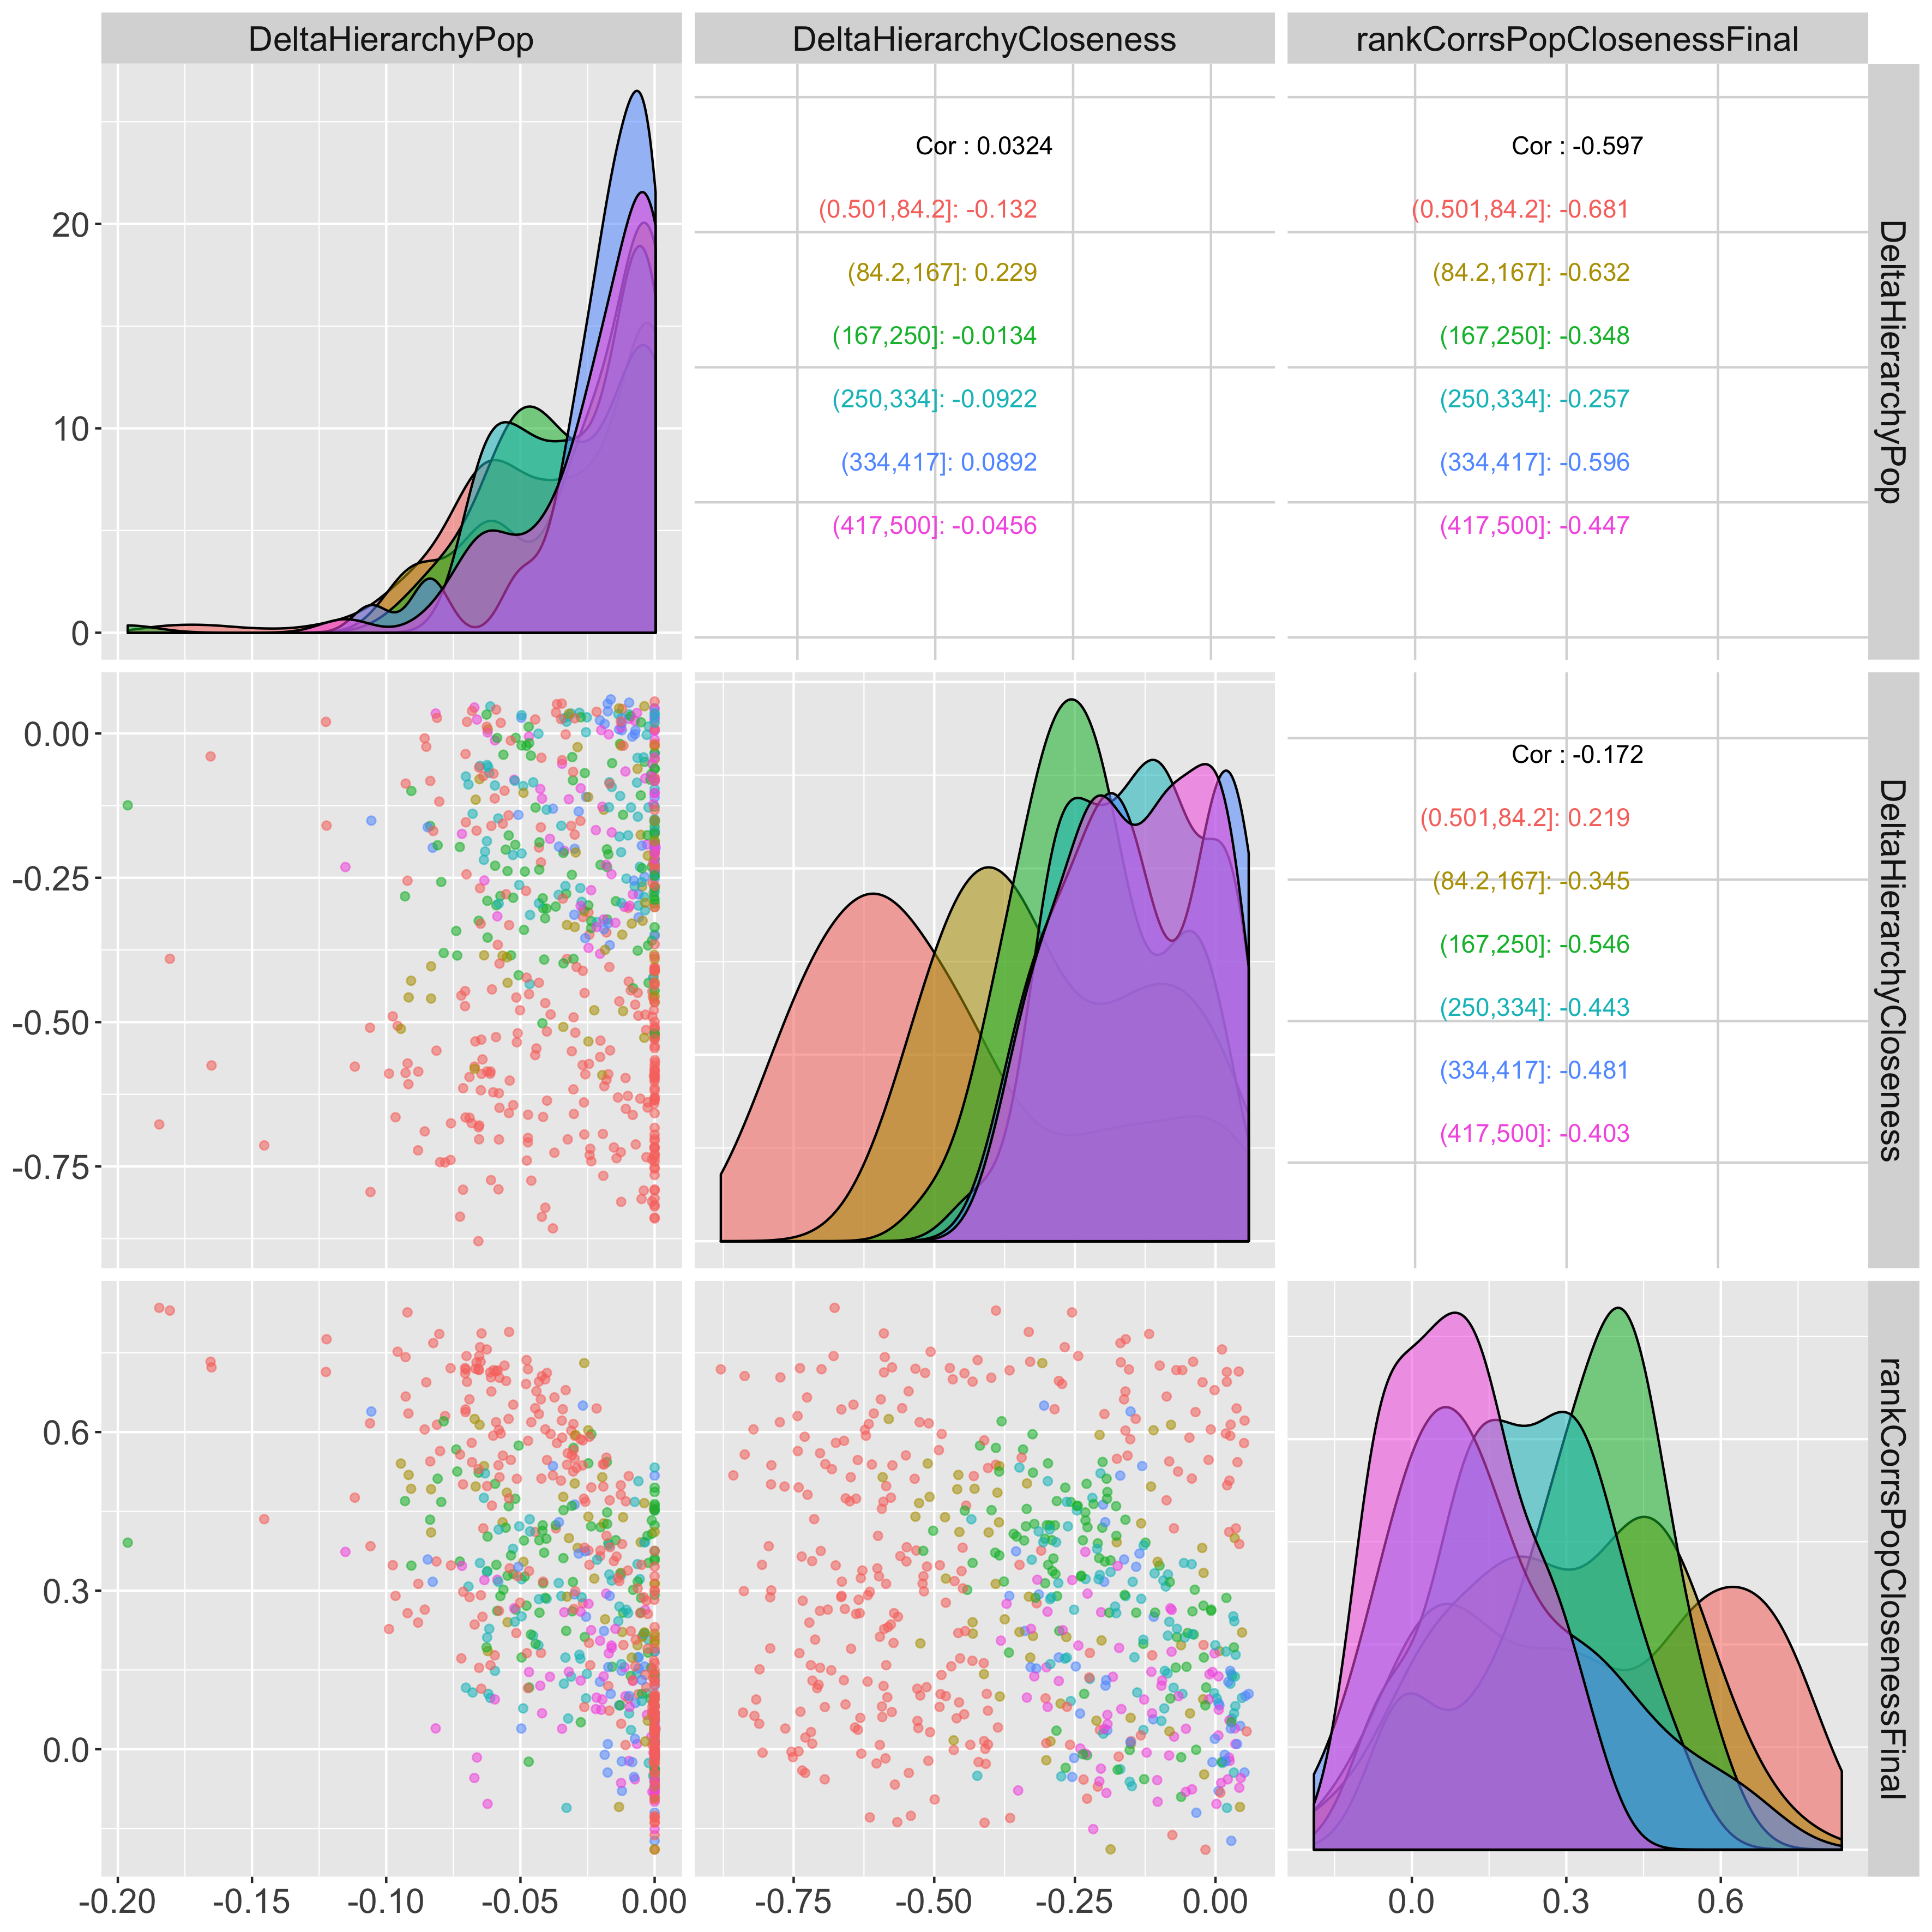
\includegraphics[width=\textwidth]{figuresraw/scatterdeltaobjs_colorgravityDecay_samples10.png}
	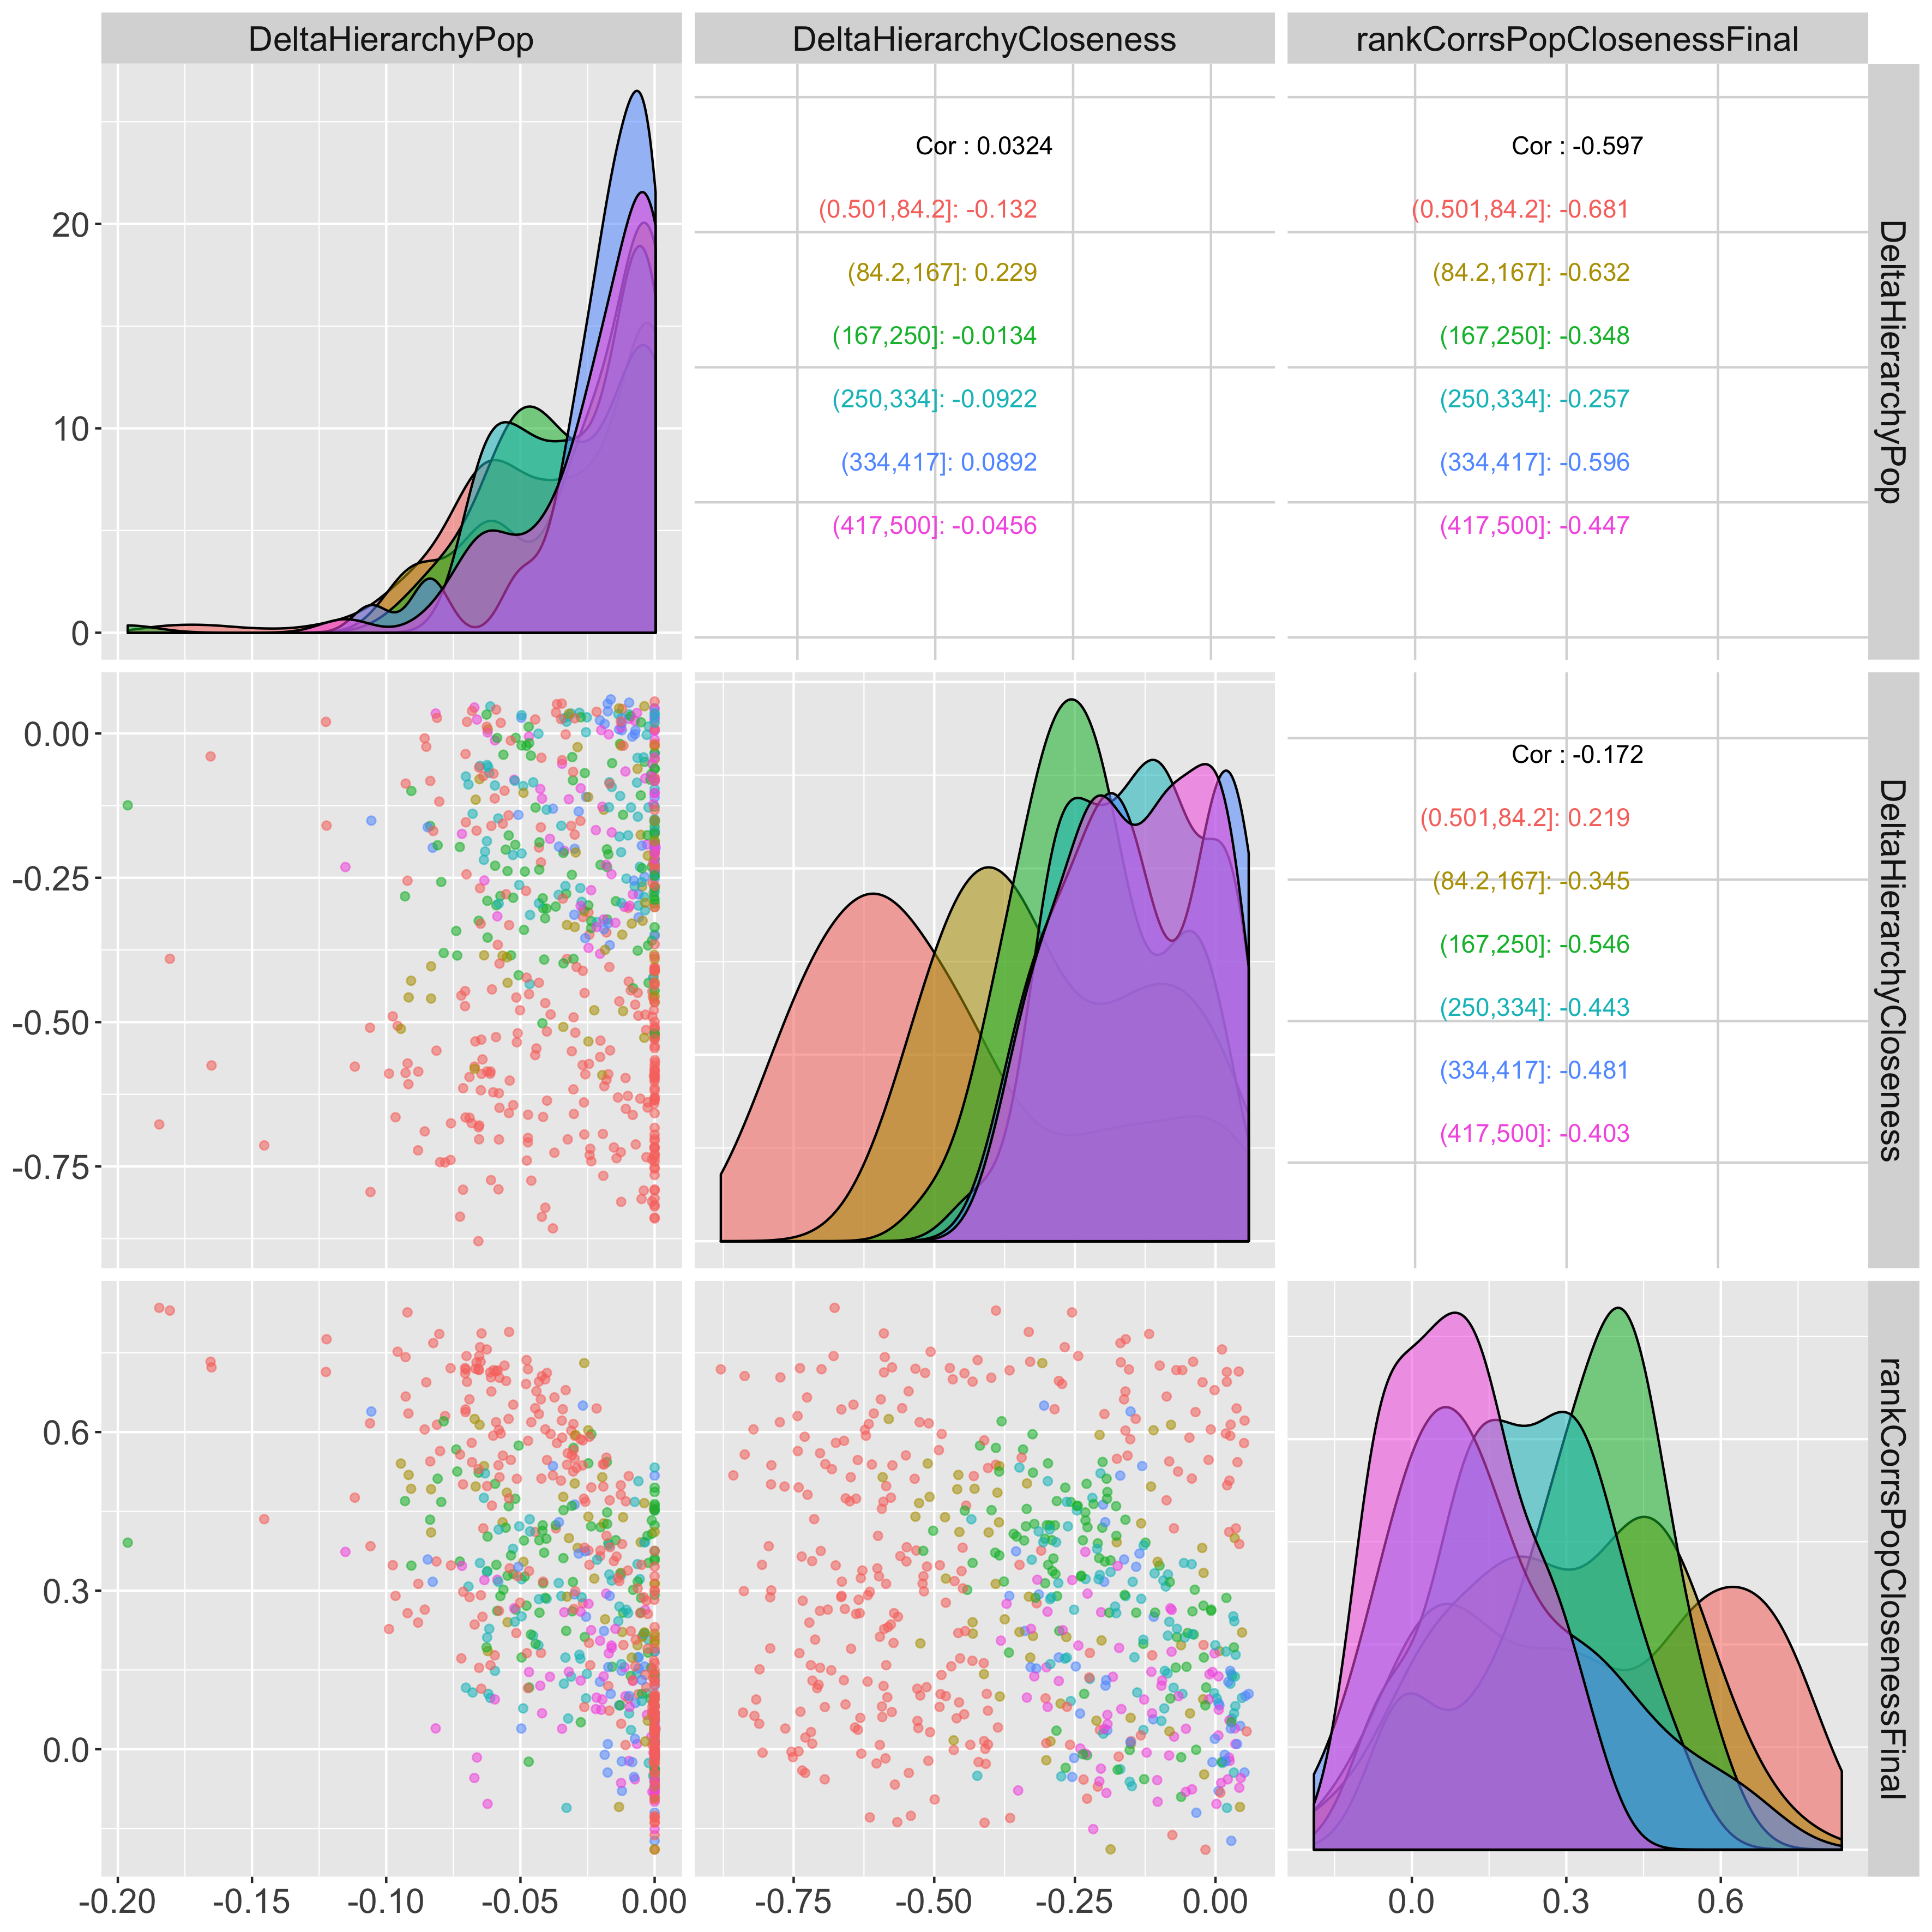
\includegraphics[width=\linewidth]{figures/Fig4.png}
	\bpar{
	\caption{\textbf{Feasible space of hierarchy regimes obtained with the PSE algorithm.} Scatter plots of the three objective dimensions. Color level gives the value of $d_G$, and distributions and correlation between indicators are also stratified following $d_G$. Patterns were filtered to have at least ten stochastic repetitions.\label{fig:pse}}
	}{
	\caption{\textbf{Espace faisable des régimes de hiérarchie obtenus par l'algorithme PSE.} Scatterplots des trois dimensions objectif. Le niveau de couleur donne la valeur de $d_G$, et les distributions et corrélations entre les indicateurs sont aussi stratifiées suivant $d_G$. Les motifs ont été filtrés pour avoir au moins dix répétitions stochastiques.\label{fig:pse}}
	}
\end{figure}
%%%%%%%%%%%%%%


\bpar{
After having inspected the link between parameters and hierarchical patterns emerging through a basic grid exploration, we turn now to a specific experiment aimed at establishing the feasible hierarchy regimes that the model can produce. Indeed in such complex simulation models, simple DOE may only capture a part of potential behavior, and miss strong non-linearities. Therefore, the Pattern Space Exploration (PSE) algorithm was introduced by \cite{cherel2015beyond} as an heuristic to approximate the feasible space of a model output, based on a novelty search algorithm \citep{lehman2008exploiting}. We apply here this algorithm with the following three dimensional pattern space: evolution of population hierarchy $\alpha_{\Delta}\left[P\right]$, evolution of centrality hierarchy $\alpha_{\Delta}\left[C\right]$, and final rank correlation between population and centrality hierarchies $\rho_r\left[P,C\right]$. For the first two, looking at dynamics is important to control for the artificial initial level of hierarchy $\alpha_S$ for population, while initial centrality hierarchy is solely linked to geometry and exhibits a narrow peak distribution of average $-0.2$ (similar pattern for virtual and physical, the physical distribution being a bit wider). These three dimension capture not only which hierarchies are produced along the two aspects included in the model, but also which relation they have in term of rank correlation.
}{
Après avoir inspecté les liens entre paramètres et motifs de hiérarchie émergents par une exploration en grille basique, nous nous tournons à présent vers une expérience spécifique visant à établir les régimes de hiérarchie faisables que le modèle peut produire. En effet dans de tels modèles complexes de simulation, des plans d'expérience simples peuvent ne capturer qu'une partie des comportements potentiels, and passer à côté de fortes non-linéarités. Pour cela, l'algorithme \emph{Patterns Space Exploration} (PSE) a été introduit par \cite{cherel2015beyond} comme une heuristique pour obtenir une approximation de l'espace faisable des sorties d'un modèle, en se basant sur un algorithme de recherche de nouveauté \citep{lehman2008exploiting}. Nous appliquons ici cet algorithme avec l'espace de motifs en trois dimensions suivant: évolution de la hiérarchie des populations $\alpha_{\Delta}\left[P\right]$, évolution de la hiérarchie des centralités $\alpha_{\Delta}\left[C\right]$, et corrélation de rang finale entre hiérarchies de population et de centralité $\rho_r\left[P,C\right]$. Pour les deux premiers, l'étude des dynamiques est important pour contrôler pour le niveau de hiérarchie initial artificiel $\alpha_S$ de la population, tandis que la hiérarchie des centralités initiale est uniquement liée à la géométrie et présente une distribution avec un pic étroit de moyenne $-0.2$ (motif similaire pour le virtuel et le physique, la distribution du physique étant un peu plus large). Ces trois dimension capturent non seulement quelles hiérarchies sont produites pour les deux aspects inclus dans le modèle, mais aussi quelle relation elles ont en termes de corrélation de rang.
}


\bpar{
We run the PSE algorithm using OpenMOLE and distribute the computation on a grid with an island scheme. The grid for patterns, set from previous exploration results, is taken as $\alpha_{\Delta}\left[P\right] \in \left[-0.2;0.2\right]$ with step $0.02$, $\alpha_{\Delta}\left[C\right] \in \left[-1.0;1.0\right]$ with step $0.1$, and $\rho_r \left[P,C\right] \in \left[-1.0,1.0\right]$ with step $0.1$. Variable parameters are aforementioned model parameters, with the addition of $g_M \in \left[0.0;0.05\right]$. The algorithm was run on 500 parallel islands (termination time 10 minutes), for $30,000$ generations (reasonable convergence in terms of number of patterns discovered).
}{
Nous exécutons l'algorithme PSE en utilisant OpenMOLE et distribuons les calculs sur une grille de calcul en utilisant un schéma par îlots. La grille pour les motifs, établie à partir des résultats d'exploration précédents, est prise comme $\alpha_{\Delta}\left[P\right] \in \left[-0.2;0.2\right]$ avec pas $0.02$, $\alpha_{\Delta}\left[C\right] \in \left[-1.0;1.0\right]$ avec pas $0.1$, et $\rho_r \left[P,C\right] \in \left[-1.0,1.0\right]$ avec pas $0.1$. Les paramètres variables sont les paramètres du modèle précédemment mentionnés, avec l'addition de $g_M \in \left[0.0;0.05\right]$. L'algorithme a été exécuté sur 500 îlots en parallèle (temps pour chaque 10 minutes), pour $30,000$ générations (convergence raisonnable en terms de nombre de motifs découverts).
}


\bpar{
We show in Fig.~\ref{fig:pse} the scatterplot of the obtained feasible space, conditionally to having at least 10 stochastic repetitions (robust patterns). We find that closeness hierarchy dynamics have a much wider range of possible values than population hierarchy dynamics, confirming what was obtained with the grid experiment. Furthermore, possible correlations have also a large span from -0.19 to 0.84, which means that the model can combine the production of a broad set of hierarchies for population and network, but also of their correlations. These correlations take mostly positive values as expected (mutual reinforcement of hierarchies), but are sometimes uncorrelated and can even be negative: in such a setting the lowest cities of the urban hierarchy have the highest centralities. These correspond to a very low initial hierarchy ($<\alpha_S>=0.18$ where the average is taken for points with a negative correlation), a high network reinforcement exponent ($<\gamma_N>=3.2$), a low interaction hierarchy ($<\gamma_G>=0.88$), and long range interactions ($<d_G>=228$). This can be interpreted as diffuse and uniform interaction in a low-hierarchical system which are mostly dominated by network processes. We can also observe in Fig.~\ref{fig:pse} for the $(\alpha_{\Delta}\left[C\right],\rho_r\left[P,C\right])$ point cloud, that around 75\% of the surface covered is by short range interactions, and correspond to extreme values: normal range interactions produce a restricted output space. Finally, it is interesting to note the upper and lower boundaries of the $(\alpha_{\Delta}\left[P\right],\rho_r\left[P,C\right])$ point cloud: population hierarchy increase fixes both kind of linear upper and lower bounds on correlations: high absolute increase of hierarchy imply high correlations, while correlations can not be too high for small variations of population hierarchy. Altogether, this experiment show a high diversity of hierarchy regimes that the model can produce.
}{
Nous montrons en Fig.~\ref{fig:pse} le nuage de points de l'espace faisable obtenu, conditionnellement à avoir au moins 10 répétitions stochastiques (motifs robustes). Nous obtenons que la hiérarchie de centralité a une plus grande plage de variation que les valeurs possibles pour les dynamiques des hiérarchie de population, ce qui confirme ce qui avait été obtenu avec l'expérience en grille. Par ailleurs, les corrélations possibles ont également une grande plage de valeur, de -0.19 à 0.84, ce qui signifie que le modèle peut combiner la production d'un large ensemble de hiérarchies pour la population et le réseau, mais aussi de leur corrélations. Ces corrélations prennent principalement des valeurs positives comme attendu (renforcement mutuel des hiérarchies), mais sont dans certains cas non corrélées, et peuvent même être négatives: dans un tel cas les villes au plus bas de la hiérarchie urbaine ont les plus grande centralités. Cela correspond à une hiérarchie initiale très basse ($<\alpha_S>=0.18$ où la moyenne est prise pour les points avec une corrélation négative), un fort exposant de renforcement du réseau ($<\gamma_N>=3.2$), une faible hiérarchie d'interaction ($<\gamma_G>=0.88$), et des interactions à longue portée ($<d_G>=228$). Cela peut être interprété comme des interaction diffuses et uniformes dans un système de faible hiérarchie qui est principalement dominé par les processus de réseau. Nous pouvons également observer en Fig.~\ref{fig:pse} pour le nuage de points $(\alpha_{\Delta}\left[C\right],\rho_r\left[P,C\right])$, que environ 75\% de la surface couverte l'est par des interactions de courte portée, et correspondent à des valeurs extrêmes: les portée d'interaction usuelles produisent un espace de sortie restreint. Enfin, il est intéressant de noter les bornes supérieure et inférieure du nuage de point $(\alpha_{\Delta}\left[P\right],\rho_r\left[P,C\right])$: un accroissement de la hiérarchie des populations impose à la fois une sorte de borne linéaire supérieur et inférieure pour les corrélations: de forts accroissements absolus de la hiérarchie impliquent de fortes corrélations, tandis que les corrélations ne peuvent pas être trop hautes pour de faibles variations de la hiérarchie des populations. En résumé, cet expérience montre une grande diversité de régimes de hiérarchie que le modèle peut produire.
}


%lm(formula = DeltaHierarchyPop ~ synthRankSize + nwThresholdQuantile + 
%    nwGmax + nwExponent + gravityWeight + gravityGamma + gravityDecay, 
%    data = res, weights = evolution.samples)
%Coefficients:
%                      Estimate Std. Error t value Pr(>|t|)    
%(Intercept)          1.039e-02  2.063e-03   5.037 4.89e-07 ***
%synthRankSize       -7.155e-03  1.436e-03  -4.984 6.44e-07 ***
%nwThresholdQuantile -8.580e-04  1.600e-03  -0.536   0.5919    
%nwGmax               7.529e-02  2.993e-02   2.516   0.0119 *  
%nwExponent          -2.126e-03  2.545e-04  -8.352  < 2e-16 ***
%gravityWeight       -6.935e+00  1.301e-01 -53.324  < 2e-16 ***
%gravityGamma        -8.179e-03  2.356e-04 -34.723  < 2e-16 ***
%gravityDecay         4.596e-05  2.490e-06  18.462  < 2e-16 ***
%Residual standard error: 0.05048 on 5208 degrees of freedom
%Multiple R-squared:  0.3967,	Adjusted R-squared:  0.3959 
%F-statistic: 489.2 on 7 and 5208 DF,  p-value: < 2.2e-16


%lm(formula = DeltaHierarchyCloseness ~ synthRankSize + nwThresholdQuantile + 
%    nwGmax + nwExponent + gravityWeight + gravityGamma + gravityDecay, 
%    data = res, weights = evolution.samples)
%Coefficients:
%                      Estimate Std. Error t value Pr(>|t|)    
%(Intercept)          1.502e-01  1.169e-02  12.848   <2e-16 ***
%synthRankSize       -6.878e-03  8.135e-03  -0.845   0.3979    
%nwThresholdQuantile -3.198e-01  9.069e-03 -35.265   <2e-16 ***
%nwGmax              -6.272e+00  1.696e-01 -36.981   <2e-16 ***
%nwExponent          -4.233e-02  1.442e-03 -29.346   <2e-16 ***
%gravityWeight        1.566e+01  7.371e-01  21.242   <2e-16 ***
%gravityGamma        -2.870e-03  1.335e-03  -2.150   0.0316 *  
%gravityDecay         5.030e-04  1.411e-05  35.648   <2e-16 ***
%Residual standard error: 0.2861 on 5208 degrees of freedom
%Multiple R-squared:  0.7016,	Adjusted R-squared:  0.7012 
%F-statistic:  1750 on 7 and 5208 DF,  p-value: < 2.2e-16

%lm(formula = rankCorrsPopClosenessFinal ~ synthRankSize + nwThresholdQuantile + 
%    nwGmax + nwExponent + gravityWeight + gravityGamma + gravityDecay, 
%    data = res, weights = evolution.samples)
%Coefficients:
%                      Estimate Std. Error t value Pr(>|t|)    
%(Intercept)         -2.659e-01  1.889e-02 -14.075  < 2e-16 ***
%synthRankSize       -1.419e-02  1.315e-02  -1.079    0.281    
%nwThresholdQuantile  8.434e-02  1.466e-02   5.753 9.25e-09 ***
%nwGmax               1.578e+00  2.742e-01   5.757 9.04e-09 ***
%nwExponent           3.226e-02  2.332e-03  13.837  < 2e-16 ***
%gravityWeight        6.546e+01  1.191e+00  54.940  < 2e-16 ***
%gravityGamma         7.558e-02  2.158e-03  35.028  < 2e-16 ***
%gravityDecay        -5.215e-04  2.281e-05 -22.863  < 2e-16 ***
%Residual standard error: 0.4624 on 5208 degrees of freedom
%Multiple R-squared:  0.4153,	Adjusted R-squared:  0.4145 
%F-statistic: 528.5 on 7 and 5208 DF,  p-value: < 2.2e-16
% Signif. codes:  0 ‘***’ 0.001 ‘**’ 0.01 ‘*’ 0.05 ‘.’ 0.1 ‘ ’ 1

%%%%%%%%%%%%%
\begin{table}
%\footnotesize
\bpar{
\caption{Linear regression analysis of model behavior based on PSE patterns. Each model is estimated with a Weighted Least Square, with weights being the number of stochastic samples. Significance levels: (***) $p \simeq 0$; (*) $p < 0.01$; () $p > 0.1$.\label{tab:regpse}}
%\begin{center}
	\begin{tabular}{@{\extracolsep{5pt}}|l|cc|cc|cc|}
%\\[-1.8ex]\hline
%\hline \\[-1.8ex]
%\\[-1.8ex]
\hline
Model & $\alpha_{\Delta}\left[P\right]$ & &  $\alpha_{\Delta}\left[C\right]$ & & $\rho_r\left[P,C\right]$ & \\ 
\hline %\\[-1.8ex] 
  Constant & $1.04\cdot 10^{-2}$ & *** & $0.15$ & *** & $-0.27$ & *** \\
  $\alpha_S$ & $-7.2\cdot 10^{-3}$ & *** & $-6.9\cdot 10^{-3}$ & & $-1.4\cdot 10^{-2}$ & \\
  $\phi_0^{(q)}$ & $-8.6\cdot 10^{-4}$ & & $-0.32$ & *** & $8.4\cdot 10^{-2}$ & *** \\
  $g_M$ & $7.5 \cdot 10^{-2}$ & * & $-6.3$ & *** & $1.6$ & *** \\
  $\gamma_N$ & $-2.1\cdot 10^{-3}$ & *** & $-4.2\cdot 10^{-2}$ & *** & $3.2\cdot 10^{-2}$ & *** \\
  $w_G$ & $-6.9$ & *** & $15.6$ & *** & $65.5$ & *** \\
  $\gamma_G$ & $-8.2\cdot 10^{-3}$ & *** & $-2.9\cdot 10^{-3}$ & * & $7.6\cdot 10^{-2}$ & *** \\
  $d_G$ &   $4.6\cdot 10^{-5}$ & *** & $5.0\cdot 10^{-4}$ & *** & $-5.2\cdot 10^{-4}$ & *** \\
  \hline% \\[-1.8ex]
Observations & 5208  & & 5208 & & 5208 & \\ 
Adjusted R$^{2}$ & 0.40 & & 0.70 & & 0.41 & \\
\hline
\end{tabular}
%\end{center}
}{
\caption{Analyse par régression linéaire du comportement du modèle basé sur les motifs de PSE. Chaque modèle est estimé par un moindre carrés pondéré, les poids étant le nombre de répétitions stochastiques. Significativité statistique: (***) $p \simeq 0$; (*) $p < 0.01$; () $p > 0.1$.\label{tab:regpse}}
%\begin{center}
	\begin{tabular}{@{\extracolsep{5pt}}|l|cc|cc|cc|}
%\\[-1.8ex]\hline
%\hline \\[-1.8ex]
%\\[-1.8ex]
\hline
Modèle & $\alpha_{\Delta}\left[P\right]$ & &  $\alpha_{\Delta}\left[C\right]$ & & $\rho_r\left[P,C\right]$ & \\ 
\hline %\\[-1.8ex] 
  Constante & $1.04\cdot 10^{-2}$ & *** & $0.15$ & *** & $-0.27$ & *** \\
  $\alpha_S$ & $-7.2\cdot 10^{-3}$ & *** & $-6.9\cdot 10^{-3}$ & & $-1.4\cdot 10^{-2}$ & \\
  $\phi_0^{(q)}$ & $-8.6\cdot 10^{-4}$ & & $-0.32$ & *** & $8.4\cdot 10^{-2}$ & *** \\
  $g_M$ & $7.5 \cdot 10^{-2}$ & * & $-6.3$ & *** & $1.6$ & *** \\
  $\gamma_N$ & $-2.1\cdot 10^{-3}$ & *** & $-4.2\cdot 10^{-2}$ & *** & $3.2\cdot 10^{-2}$ & *** \\
  $w_G$ & $-6.9$ & *** & $15.6$ & *** & $65.5$ & *** \\
  $\gamma_G$ & $-8.2\cdot 10^{-3}$ & *** & $-2.9\cdot 10^{-3}$ & * & $7.6\cdot 10^{-2}$ & *** \\
  $d_G$ &   $4.6\cdot 10^{-5}$ & *** & $5.0\cdot 10^{-4}$ & *** & $-5.2\cdot 10^{-4}$ & *** \\
  \hline% \\[-1.8ex]
Observations & 5208  & & 5208 & & 5208 & \\ 
R$^{2}$ ajusté & 0.40 & & 0.70 & & 0.41 & \\
\hline
\end{tabular}
%\end{center}
}

\end{table}
%%%%%%%%%%%%%


\bpar{
Finally, as the output produced by the PSE algorithms are assumed to be mostly representative of what the model can offer, we can expect statistical models linking parameters and indicators to capture most of its behavior. We propose therefore in Table~\ref{tab:regpse} a linear regression analysis of model behavior. The estimation is done on the full PSE population but with weighting according to the number of stochastic samples, in order to avoid bias by non robust patterns. Most of variations explained in the grid experiment are confirmed, as hierarchies increasing with $d_G$, or decreasing with $\gamma_G$. The overall behavior of correlations is opposed to what was observed as a function of $d_G$ since it decreases. It is also interesting to note that centrality hierarchy and correlation are not significant in $\alpha_S$, while population hierarchy is not significant in $\phi_0^{(q)}$: on these dimensions, the intrication between cities and the transportation network is not statistically effective for a linear model (since these non-significant link occur between city indicator and network parameter on the one hand, and between network indicator and city parameter on the other hand).
}{
Enfin, comme la sortie produite par l'algorithme PSE peut être attendue comme principalement représentative de ce que le modèle peut offrir, nous pouvons attendre de modèles statistiques reliant paramètres et indicateurs de capturer la plupart de son comportement. Nous proposons pour cela en Table~\ref{tab:regpse} une analyse par régression linéaire du comportement du modèle. L'estimation est faite sur la population de PSE complète mais avec une pondération selon le nombre de répétitions stochastiques, afin d'éviter un biais produit par les motifs non-robustes. La plupart des variations expliquées dans l'expérience de grille sont confirmées, comme les hiérarchies croissantes avec $d_G$, ou décroissantes avec $\gamma_G$. Le comportement global des correlations s'oppose à ce qui était observé en fonction de $d_G$ puisqu'il décroit. Il est également intéressant de noter que la hiérarchie des centralités et la corrélation ne sont pas significatifs en fonction de $\alpha_S$, tandis que la hiérarchies des populations n'est pas significative en $\phi_0^{(q)}$: pour ces dimensions, l'intrication entre villes et réseau de transport n'est pas statistiquement effective pour un modèle linéaire (puisque ces liens non significatifs se produisent entre indicateur de ville et paramètres de réseau d'une part, et entre indicateur de réseau et paramètre de ville d'autre part).
}






%%%%%%%%%%%%%%%%
\bpar{
\section{Discussion}
}{
\section{Discussion}
}



%\subsection{Results on co-evolution and hierarchies}

% what do we learn in this particular context ?
% - teachings on the role of self-reinforcement

% 1) pop hierarchy depends on network, in a non monotnous way (intermediate interaction range for example)
% 2) correlation
% 

\bpar{
Our model exploration results have implications on the thematic question of hierarchy in urban systems and the role of co-evolution between cities and networks in its dynamics. We showed several stylized fact which have non trivial implications, including: (i) the fact that urban hierarchy depends on network processes, and that in some cases this link is non-monotonous - what introduces an additional complexity in planning such infrastructures at a macroscopic scale if put in a long time co-evolutionary context; (ii) the fact that correlation between urban hierarchy and network hierarchy are most of the time positive, but that it can take a broad range of values and even be negative - this also challenges the reductionist view of a direct correspondance between the hierarchy of a city and its accessibility, since the link depends of several parameters and of the type of interactions considered; (iii) the fact that conclusions obtained with the physical network model are globally qualitatively similar to the conclusions obtained with the virtual network, but that behavior still significantly differs in some regions of the parameter space for some indicators - what means that in some case such a simplification will be fine to be done while in other it will miss some crucial processes; (iv) the fact that the realm of possible hierarchy regimes is very broad, surely much broader than existing regimes.
}{
Nos résultats d'exploration de modèle ont des implications pour la question thématique de la hiérarchie dans les systèmes urbains et le rôle de la co-évolution entre villes et réseaux dans ses dynamiques. Nous avons montré un certain nombre de faits stylisés qui ont des implications non triviales, incluant: (i) le fait que les hiérarchies urbaines dépendent des processus de réseau, et que dans certains cas ce lien est non-monotone - ce qui introduit une complexité supplémentaire pour la planification de telles infrastructures à une échelle macroscopique lorsque un contexte de temps long avec processus de co-évolution est considéré; (ii) le fait que les corrélations entre hiérarchie urbaine et hiérarchie de réseau sont la plupart du temps positives, mais qu'elles peuvent prendre une large gamme de valeurs et peuvent même être négatives - cela questionne également la vision réductionniste d'une correspondence directe entre la hiérarchie d'une ville et son accessibilité, puisque le lien dépend de nombreux paramètres et du type d'interactions considérées; (iii) le fait que les conclusions obtenues avec le réseau physique sont globalement qualitativement similaires aux conclusions obtenues avec le réseau virtuel, mais que le comportement diffère cependant significativement dans certaines parties de l'espace des paramètres pour certains indicateurs - ce qui signifie que dans certains cas une telle simplification sera acceptable tandis que dans d'autres elle passera à côté de processus cruciaux; (iv) le fait que le domaine des régimes de hiérarchie possibles est très vaste, sûrement plus étendu que les régimes existant en pratique.
}


\bpar{
This last point opens the issue of comparing this approach with data and possibly identifying hierarchy regimes in existing urban systems. \cite{raimbault2018modeling} have applied this model to real population data and real rail network distance matrices in the case of the French urban system, by calibrating it on population and distance trajectories. As the model is fitted on a moving window in time, the temporal trajectory of fitted parameters may inform on the actual regime the urban system is in. However, such conclusions would be more robust if applied on different urban systems, as \cite{raimbault2019evolutionary} do for six large urban systems when benchmarking similar interaction growth models. A purely empirical characterization of hierarchy regimes, using indicators introduced here, would also be a relevant entry to this issue, but the lack of transportation data on long time scales and broad spatial spans remains an obstacle difficult to overcome. 
}{
Ce dernier point ouvre la question de comparer cette approche avec des données et possiblement identifier les régimes de hiérarchie dans des systèmes urbains existants. \cite{raimbault2018modeling} a appliqué ce model aux données réekkes de population et de matrices de distance du réseau ferré dans le cas du système urbain français, en le calibrant sur les trajectoires de population et de distance. Comme le modèle est ajusté sur une fenêtre temporelle glissante dans le temps, la trajectoire temporelle des paramètres ajustés peut informer sur le régime effectif dans lequel le système urbain est. Cependant, de telles conclusions seraient plus robustes si appliquées sur différents systèmes urbains, comme \cite{raimbault2019evolutionary} le fait pour six grand systèmes urbains pour comparer des modèles similaire de croissance par interaction. Une caractérisation purement empirique des régimes de hiérarchie en utilisant les indicateurs décrits ici serait également une entrée intéressante pour cette question, mais le manque de données de transport sur de longues échelles temporelles et de grandes étendues spatiales reste un obstacle difficile à surmonter.
}

%\subsection{Developments}

%\subsection{Spatial hierarchical niches}
% possible experiment: optim algo to isolate optimal fitting niches; find typical niche size when varying parameters
% (out of the scope / development of algo in itself)

% the model add no links! -> in a way very similar to Levinson? - other scale and other purpose / measures

\bpar{
The methodology to understand hierarchical patterns in systems of cities, and the model itself are also prone to several potential developments. For example, the idea of spatial non-stationarity in estimating scaling laws, which would in a sense be linked to the existence of urban subsystems with their own hierarchical patterns, should be developed in methodological terms. An heuristic to optimize the adjustment of such a non-stationary model has to be introduced, and may be difficult to elaborate since a spatial neighborhood is not necessarily the rule in constituting subsystems of cities (large global metropolises may be a subsystem linked tighter than one of these with its hinterland in Europe for example). This then also relates to issues of relevant scales to identify hierarchies. Regarding the model in itself, it remains very simple and not realistic in the sense that similarly to \citep{xie2009topological}, no link are added, but only the speeds of existing links are updated. On the contrary, road network growth models at other scales such as \cite{raimbault2019urban} focus on the addition of links. Bridging these two approaches would be a relevant extension of the model studied here.
}{
La méthodologie pour comprendre les motifs de hiérarchie dans les systèmes de villes, et le modèle en lui-même, sont également potentiellement porteurs de développements. Par exemple, l'idée de la non-stationnarité spatiale dans l'estimation des lois d'échelles, qui serait en un sens liée à l'existence de sous-systèmes urbains avec leurs propres motifs hiérarchiques, devrait être développée en termes méthodologiques. Une heuristique pour optimiser l'ajustement d'un tel modèle non-stationnaire doit être introduite, et peut être difficile à élaborer puisqu'un voisinage spatial n'est pas nécessairement la règle pour constituer des sous-systèmes de villes (les grandes métropoles globalisées peuvent être un sous-système aux liens plus forts que l'une de ces villes et sont hinterlnd en Europe par exemple). Cela évoque ensuite aussi le problème des échelles pertinentes pour identifier les hiérarchies. Concernant le modèle en lui-même, il reste très simple et peut réaliste au sens où de manière similaire à \citep{xie2009topological}, aucun lien n'est ajouté, mais seulement les vitesses des liens existants sont mises à jour. Au contraire, les modèles de croissance des réseaux routiers à d'autres échelles comme \cite{raimbault2019urban} se concentrent sur l'ajout de lien. Un pont entre ces deux approches serait une extension pertinente du modèle étudié ici.
}


%\subsection{Theoretical perspective}

% ~ disc from jig ?

% \textbf{Proposition : } \textit{les hiérarchies, au sens d'imbrication de sous-systèmes à de multiples niveaux, sont endogènes aux systèmes complexes}
% des structures ``hiérarchiques'' au sens commun (structure de dépendance rigide et arborescente) sont simples et ni adaptatives ni résilientes
% le concept de hiérarchie ne peut être considéré comme exogène et totalement déconstruit
% pour l'aide à la décision, des utopies réductionnistes en horizontalité complète s'opposent aux théories de la complexité
% question ouverte (reflexive): endogènes \textit{aux systèmes} ou aux \textit{théories et modèles des systèmes} ?
%\textbf{Des approches multi-scalaires intégratives pour des gouvernances territoriales soutenables \cite{rozenblat2018conclusion} doivent prendre en compte la complexités des hiérarchies.}


\bpar{
Finally, our results can be put into a wider theoretical perspective. As explained in introduction, hierarchies in the sense of the imbrication of subsystems at multiple levels, are endogenous to complex systems. At a fixed scale, quantitative indicators such as the one we used capture emergent patterns of this organisation, as is the hierarchical structure in systems of cities in terms of scaling laws. Thus, to understand and manage such systems in a resilient and adaptive way, multi-scale approaches embracing these hierarchies are necessary, as put forward by \cite{rozenblat2018conclusion}. Our model is a first suggestion of scale integrations, since in the physical network case cities are at the macroscopic scale while the network is at a finer mesoscopic scales.
}{
Enfin, nos résultats peuvent être vus dans une perspective théorique plus large. Comme expliqué en introduction, les hiérarchies au sens de l'imbrication de sous-systèmes à de multiples niveaux, sont endogènes aux systèmes complexes. A une échelle fixée, des indicateurs quantitatifs tel que ceux utilisés capturent des motifs émergents de cette organisation, comme l'est la structure hiérarchique des systèmes de villes en termes de lois d'échelle. Ainsi, pour comprendre et gérer de tels systèmes de façon résiliante et adaptative, des approches multi-échelle capturant ces hiérarchies sont nécessaires, comme suggéré par \cite{rozenblat2018conclusion}. Notre modèle est une première suggestion d'intégration des échelles, puisque dans le cas du réseau physique les villes sont à l'échelle macroscopique tandis que le réseau est à une échelle mesoscopique plus fine.
}



%%%%%%%%%%%%%%%%
\bpar{
\section{Conclusion}
}{
\section{Conclusion}
}

\bpar{
We explored here the concept of hierarchy in the particular context of the co-evolution of transportation networks and cities. More particularly, we introduced a set of indicators to quantify hierarchy patterns, and systematically studied a co-evolution model for cities and networks, at two abstraction levels for the network. Our exploration results provide some non trivial stylized facts and inform on the diversity of regimes the model can produce. This provides an illustration of how to study hierarchy in territorial systems regarding two complementary dimensions, in terms of how each hierarchically organizes and what is the actual correspondance between the two hierarchies.
}{
Nous avons exploré ici le concept de hiérarchie dans le contexte particulier de la co-évolution des réseaux de transport et des villes. Plus particulièrement, nous avons introduit un jeu d'indicateurs pour quantifier les motifs de hiérarchie, et étudié systématiquement un modèle de co-évolution pour les villes et les réseaux, à deux niveaux d'abstraction pour le réseau. Nos résultats d'exploration donnent des faits stylisés non triviaux et informent sur la diversité des régimes que le modèle peut produire. Cela fournit une illustration de comment étudier la hiérarchie dans les systèmes territoriaux selon deux dimensions complémentaires, selon comment chacune s'organise hiérarchiquement et quelle est la correspondence effective entre les deux hiérarchies.
}


%%%%%%%%%%%%%%%%
\bpar{
\section{Acknowledgements}
}{
\section{Remerciements}
}

\bpar{
Results obtained in this paper were computed on the vo.complex-system.eu virtual organization of the European Grid Infrastructure ( http://www.egi.eu ). We thank the European Grid Infrastructure and its supporting National Grid Initiatives (France-Grilles in particular) for providing the technical support and infrastructure. This work was funded by the Urban Dynamics Lab grant EPSRC EP/M023583/1.
}{
Les résultats obtenus dans ce chapitre on été calculés sur l'organisation virtuelle vo.complex-system.eu de la European Grid Infrastructure ( http://www.egi.eu ). Nous remercions la European Grid Infrastructure et ses initiatives de support nationales (France-Grilles en particulier) de fournir le support technique et l'infrastructure. Ce travail a été financé par la bourse Urban Dynamics Lab EPSRC EP/M023583/1.
}




\bibliographystyle{agsm}
\bibliography{biblio}
%\def\pagesname{pp.~}
%\def\numbername{no.~}
%\def\pagename{p.~}



%\appendix
%\chapter{Appendix}



%\vfill\pagebreak
%\
%\thispagestyle{empty}


\end{document} 


%%%%%
%% Template 

%\begin{figure}[ptbh]
%\centering
%\includegraphics[width=10.6009cm,height=4.714cm]{GadalaExp.eps}\caption{Start and stop shear flow experiment;\break the torque would be proportional
%to the shear stress, after\break Gadala-Maria and Acrivos \cite{Gadala80}}
%\label{Fig 1}
%\end{figure}\pagebreak




